\documentclass[UTF8]{ctexart}

\makeatletter
\def\input@path{{../../Fulcrum-Template/}{../../Operator-List/}}
\makeatother

\usepackage{FulcrumHabitCN}
\usepackage{OperatorListCN}
\usepackage{F4LinearAlgebra}

\begin{document}
  
\tableofcontents
\newpage

\section{向量和\线性空间}
	\subsection{\数域}
		\begin{dfn}
			[Number-Field]
			{\数域}
			[Number Field]
			[]
        
			一个\数域$\K$称为是一个\textbf{\数域(Number Field)}, 若在$\K$上定义了两种$\K^2\to
            \K$的二元运算加法"$+$"和乘法"$\cdot$", 满足: 
			
			(1)$\K$对加法运算封闭: 
			$$\forall a,b\in \K, a+b\in \K$$
			
			(2)有一种加法运算的逆运算"$-$", 且$\K$对该减法运算封闭: 
			$$\forall a,b\in \K, \exists (b-a)\in \K: a+(b-a)=b$$
			
			(3)$\K$对乘法运算封闭: 
			$$\forall a,b\in \K, a\cdot b\in \K$$
			
			(4)有一种乘法运算的逆运算"$/$", 且$\K$对除数不为零的除法运算封闭: 
			$$\forall a,b\in \K(a\neq 0), \exists (b/a)\in \K: a\cdot(b/a)=b$$
		\end{dfn}	
			
		\begin{thm}
            []
			{最小的无限\数域}
        	[]
			[]

			全体无限\数域 的交集为有理\数域$\mathbb{Q}$. \textit{(有理\数域 是“最小”的无限\数域)}
		\end{thm}
        \begin{prf}设$\K$是一个非空无限\数域. 
			
			$$\because \K\neq \varnothing$$
			
			$$\Longrightarrow \exists 1 \in \K$$
			
			$$\Longrightarrow \underbrace{1+1+\cdots +1}_{n\mbox{个}1}=n \in \K$$
			
			$$\Longrightarrow -n\in \K$$
			
			$$\Longrightarrow 0=n+(-n)\in \K$$
			
			$$\Longrightarrow \Z \subseteq \K$$
			
			$$\Longrightarrow \forall \frac{p}{q}\in \mathbb{Q}(p,q\in \Z\subseteq \K, q\neq 0, \gcd(p,q)=1), \frac{p}{q}=p/q \in \K$$
			
			$$\Longrightarrow \mathbb{Q} \subseteq \K$$
			
			又$\because \mathbb{Q}$是\数域, 
			
			$\Longrightarrow \mathbb{Q}$全体无限\数域 的交集为有理\数域. $\square$
        \end{prf}
			
	\subsection{向量和\线性空间}
		\begin{dfn}
			[Linear-Space]
			{\线性空间}
			[Linear Space]
			[]

			集合$V$称为是一个\textbf{\数域$\K$上的\线性空间(Linear Space on Number Field $\K$)}, 简称\textbf{\线性空间(Linear Space)}, V中的元素称为\textbf{向量(vector)}, 若在$V$上定义了两种运算: 加法"+": $V\times V\to V$ 和数乘: $\K\times V \to V$, 满足:

			(1)加法交换律成立: 
			\[\forall \alpha,\beta \in V, \alpha+\beta=\beta+\alpha\]

			(2)加法结合律成立: 
			\[\forall \alpha,\beta, \gamma \in V, \alpha+(\beta+\gamma)=(\alpha+\beta)+\gamma\]
			
			* 上述等式通常记为$\alpha+\beta+\gamma$. 

			(3)加法恒等元存在: 
			\[\exists e\in V, \forall \alpha \in V, \alpha +e=\alpha\]
			
			* 加法恒等元通常记为$\mathbf{0}$, 称为\textbf{零向量}, $\mathbf{0}\neq 0$, $\mathbf{0}$是向量, $0$是数. 

			(4)加法逆元存在: 
			\[\forall \alpha \in V, \exists \beta \in V: \alpha+\beta=\mathbf{0}\]
			
			* 加法逆元通常称为$\alpha$的\textbf{负向量}, 记为$-\alpha$. 

			(5)数乘结合律成立: 
			\[\forall k,l\in \K, \forall \alpha \in V, k(l\alpha) =(kl)\alpha\]
			
			* 上述等式通常记为$kl\alpha$. 

			(6)数乘分配律对$V$中的元素成立: 
			\[\forall k\in \K, \forall \alpha , \beta \in V, k(\alpha +\beta)=k\alpha+k\beta\]

			(7)数乘分配律对\数域$\K$中的数成立: 
			\[\forall k,l\in \K, \forall \alpha \in V, (k+l)\alpha =k\alpha +l\alpha\]
			
			(8)数乘恒等元存在: 
			\[\exists 1\in \K: \forall \alpha \in V, 1\alpha=\alpha\]
		\end{dfn}
		
		\begin{ppt}
			[]
			{零向量的唯一性}
			[]
			[]

			\线性空间$V$中的零向量$\mathbf{0}$唯一
		\end{ppt}
        \begin{prf}设$\exists \mathbf{0}, \mathbf{0}' \in V$, 且它们都是\线性空间$V$零向量, 则: 
			\[\mathbf{0}=\mathbf{0}+\mathbf{0}'=\mathbf{0}'\]
			
			即零向量唯一. $\square$ 
        \end{prf}
		
		\begin{ppt}
			[]
			{负向量的唯一性}
			[]
			[]

			$\forall \alpha \in V$, $\alpha$的负向量$-\alpha$唯一
		
		\end{ppt}
        \begin{prf}设$\exists -\alpha, (-\alpha)' \in V: \alpha+ (-\alpha)= \alpha + (-\alpha)'=\mathbf{0}$, 则: 
			$$-\alpha= -\alpha + \alpha + (-\alpha)'=(-\alpha)'$$
			
			即$\alpha$的负向量唯一. $\square$ 
        \end{prf}
		
		\begin{ppt}
			[]
			{加法消去律成立}
			[]
			[]

			$$\forall \alpha, \beta, \gamma \in V, \alpha +\gamma = \beta +\gamma \Longrightarrow \alpha =\beta$$
		\end{ppt}
        \begin{prf}
            左右两式同加$-\gamma$, 得: \[\alpha +\gamma -\gamma = \beta +\gamma -\gamma\]
			
			即$\alpha =\beta$. $\square$ 
         \end{prf}
		
		\begin{ppt}
			[]
			{0乘以任意向量等于零向量}
			[]
			[]

			$$\forall \alpha \in V, 0\alpha =\mathbf{0}$$
		\end{ppt}
        \begin{prf}
		证明: 
		
		 	$$0\alpha = (0+0)\alpha = 0\alpha + 0\alpha \Longrightarrow 0\alpha = \mathbf{0}\square$$
        \end{prf}
		
		\begin{ppt}
			[]
			{任意数乘以零向量等于零向量}
			[]
			[]

			$$\forall k \in \K, k\mathbf{0}=\mathbf{0}$$
		\end{ppt}
        \begin{prf}
            \[k\mathbf{0}=k(\mathbf{0}+\mathbf{0})=k\mathbf{0}+k\mathbf{0}\Longrightarrow k\mathbf{0}=\mathbf{0}\square\]
        \end{prf}
		
		\begin{ppt}
			[]
			{-1乘以任意向量等于负向量}
			[]
			[]

			$$\forall \alpha \in V, (-1)\alpha=-\alpha$$
		\end{ppt}
        \begin{prf}
            \[(-1)\alpha+\alpha=[(-1)+1]\alpha=0\alpha=\mathbf{0}\Longrightarrow (-1)\alpha=-\alpha\square\]
        \end{prf}
		
		\begin{ppt}
			[]
			{一个数与一个向量相乘为零向量,当且仅当数为零或向量为零向量}
			[]
			[]

			$$k\alpha=\mathbf{0}\Longrightarrow k=0\mbox{或}\alpha=\mathbf{0}$$
		\end{ppt}
  
        \begin{prf}
		    若$k=0$, 则结论已经成立; 
			设$k\neq 0$, 则$\exists k^{-1}\in \K: kk^{-1}=1$, 则: 
			
			$$\alpha=(kk^{-1})\alpha=k^{-1}(k\alpha)=k^{-1}\mathbf{0}=\mathbf{0}$$
			
			$$\Longrightarrow k\neq 0\Longrightarrow \alpha=\mathbf{0}$$
		
			即$k\alpha=\mathbf{0}\Longrightarrow k=0\mbox{或}\alpha=\mathbf{0}$. $\square$
        \end{prf}
	
	\subsection{向量的线性关系}
		\begin{dfn}
			[Linear-Combination]
			{\线性组合}
			[Linear Combination]
			[]
			
			设$V$是\数域$\K$上的\线性空间, $\alpha_{1}, \alpha_{2}, \cdots, \alpha_{n}, \beta \in V$. 
			
			$\beta$称为是$\alpha_{1}, \alpha_{2}, \cdots, \alpha_{n}$的\textbf{\线性组合(Linear Combination)}, 或称$\beta$可由$\alpha_{1}, \alpha_{2}, \cdots, \alpha_{n}$\textbf{线性表示(Linearly Expressed)}, 若: 
			
			$$\exists k_{1}, k_{2}, \cdots, k_{n}\in \K: \beta = \sum_{i=1}^{n}k_{i}\alpha_{i}$$
			
			称向量组$A$可由向量组$B$线性表示, 若$\forall\alpha\in A, \alpha$能被$B$线性表示. 
		
		\end{dfn}
		
		\begin{dfn}
			[Linearly-Related]
			{\线性相关}
			[Linearly Related]
			[]
		
			设$V$是\数域$\K$上的\线性空间, $\alpha_{1}, \alpha_{2}, \cdots, \alpha_{n}\in V$. 
		
			向量组$\{\alpha_{1}, \alpha_{2}, \cdots, \alpha_{n}\}$称为是\textbf{\线性相关(Linearly Related)}的, 若: 
		
			$$\exists k_{1}, k_{2}, \cdots, k_{n}\in \K: k_{1}, k_{2}, \cdots, k_{n}\mbox{不都}=0: \sum_{i=1}^{n}k_{i}\alpha_{i}=\mathbf{0}$$
			
			向量组$\{\alpha_{1}, \alpha_{2}, \cdots, \alpha_{n}\}$称为是\textbf{线性无关(Linearly Independent)}的, 若: 
		
			$$\exists k_{1}, k_{2}, \cdots, k_{n}\in \K: \sum_{i=1}^{n}k_{i}\alpha_{i}=\mathbf{0}\Longleftrightarrow k_{1}=k_{2}=\cdots=k_{n}=0$$
			
		\end{dfn}
		
		\begin{ppt}
			[]
			{\线性相关 和线性无关的等价定义}
			[]
			[]
			
			向量组$A=\{\alpha_{1}, \alpha_{2}, \cdots, \alpha_{n}\}$\线性相关 $\Longleftrightarrow \exists \alpha_{i} \in A:\alpha_{i}$可被$A-\{\alpha_{i}\}$线性表示; 
			
			向量组$A=\{\alpha_{1}, \alpha_{2}, \cdots, \alpha_{n}\}$线性无关 $\Longleftrightarrow \forall \alpha_{i} \in A:\alpha_{i}$不可被$A-\{\alpha_{i}\}$线性表示. 
		
		\end{ppt}
		\begin{prf}
		    (1)若向量组$A=\{\alpha_{1}, \alpha_{2}, \cdots, \alpha_{n}\}$\线性相关, 则: 
			
			$$\exists k_{1}, k_{2}, \cdots, k_{n}\in \K: k_{1}, k_{2}, \cdots, k_{n}\mbox{不都}=0: \sum_{i=1}^{n}k_{i}\alpha_{i}=\mathbf{0}$$
			
			$$\Longrightarrow \exists k_{i}\in {k_{1}, k_{2}, \cdots, k_{n}}: k_{i}\neq 0$$
			
			$$\Longrightarrow \sum_{j=1, j\neq i}^{n}k_{j}\alpha_{j}=-k_{i}\alpha _{i}$$
			
			$$\because k_{i}\neq 0, \Longrightarrow \exists k_{i}^{-1}\in \K: k_{i}k_{i}^{-1}=(1) $$
			
			$$\Longrightarrow \alpha_{i}=-k_{i}^{-1}\sum_{j=1, j\neq i}^{n}k_{j}\alpha_{j}= \sum_{j=1, j\neq i}^{n}-\frac{k_{j}}{k_{i}}\alpha_{j}$$
			
			即$\exists \alpha_{i} \in A:\alpha_{i}$可被$A-\{\alpha_{i}\}$线性表示; 
			
			(2) 若$\exists \alpha_{i} \in A:\alpha_{i}$可被$A-\{\alpha_{i}\}$线性表示, 则: 
			
			$$\alpha_{i}=\sum_{j=1, j\neq i}^{n}k_{j}\alpha_{j}$$
			
			$$k_{i}:=-1, \sum_{j=1}^{n}k_{j}\alpha_{j}=\mathbf{0}$$
			
			即$A$\线性相关. 
			
			由于线性无关与\线性相关 为互补关系, 运用反证法可直接证明关于线性无关的等价定义也是成立的. $\square$
        \end{prf}
			
		\begin{ppt}
			[]
			{\线性相关 和线性无关的另一等价定义}
			[]
			[]
			
			向量组$A=\{\alpha_{1}, \alpha_{2}, \cdots, \alpha_{n}\}$线性无关$\Longleftrightarrow \forall \beta: \beta$可被$A$线性表示, 这种表示唯一; 
			
			向量组$A=\{\alpha_{1}, \alpha_{2}, \cdots, \alpha_{n}\}$\线性相关$\Longleftrightarrow \forall \beta: \beta$可被$A$线性表示, 这种表示不唯一. 
						
		\end{ppt}
		\begin{prf}
  
	       (1)若向量组$A=\{\alpha_{1}, \alpha_{2}, \cdots, \alpha_{n}\}$线性无关, 则: 
			
			设$\beta$可被$A$线性表示, 有: 
			
			$$\beta :=\sum_{i=1}^{n}k_{i}\alpha_{i} =\sum_{i=1}^{n}k_{i}'\alpha_{i}$$
			
			$$\sum_{i=1}^{n}k_{i}\alpha_{i} -\sum_{i=1}^{n}k_{i}'\alpha_{i}=\sum_{i=1}^{n}(k_{i}-k_{i}')\alpha_{i}=\mathbf{0}$$
			
			$$\sum_{i=1}^{n}(k_{i}-k_{i}')\alpha_{i}=\mathbf{0}\Longrightarrow k_{i}-k_{i}'=0\Longrightarrow k_{i}=k_{i}'(i=1,2,\cdots ,n)$$
			
			即$\beta$被$A$表示方式唯一. 
			
			(2)若向量组$A=\{\alpha_{1}, \alpha_{2}, \cdots, \alpha_{n}\}$\线性相关, 则: 
			
			$$\exists k_{1}, k_{2}, \cdots, k_{n}\in \K: k_{1}, k_{2}, \cdots, k_{n}\mbox{不都}=0: \sum_{i=1}^{n}k_{i}\alpha_{i}=\mathbf{0}$$
			
			设$\beta$可被$A$线性表示, 有: 
			
			$$\beta :=\sum_{i=1}^{n}l_{i}\alpha_{i}$$
			
			$$\because \forall k\in \K, k\mathbf{0}+\beta=\beta$$
			
			$$\Longrightarrow \beta =k\sum_{i=1}^{n}k_{i}\alpha_{i}+\sum_{i=1}^{n}l_{i}\alpha_{i}=\sum_{i=1}^{n}(kk_{i}+l_{i})\alpha_{i}$$
			
			$\because k_{i}$不全为零, $\Longrightarrow \beta$的表示方式不唯一. 
			
			由于线性无关与\线性相关 为互补关系, 运用反证法可直接证明对于必要性情况的等价定义也是成立的. $\square$
		\end{prf}
  
		\begin{ppt}
			[]
			{\线性相关 的包含性}
			[]
			[]
			若向量组$A=\{\alpha_{1}, \alpha_{2}, \cdots, \alpha_{n}\}$线性无关, 则$\forall$向量组$B\subseteq A$, 有$B$线性无关. 
			若向量组$A=\{\alpha_{1}, \alpha_{2}, \cdots, \alpha_{n}\}$\线性相关, 则$\forall$向量组$B\supseteq A$, 有$B$线性相关. 
						
		\end{ppt}
		\begin{prf}
		
			(1)运用反证法. 
			
			设$A$线性无关而$B\subseteq A$\线性相关, 则: 
			
			$$\exists \alpha_{i}\in B: \alpha_{i}\mbox{能被}B-\alpha_{i}\mbox{线性表示}$$
			
			$$\because B-\alpha_{i}\subseteq A-\alpha_{i}$$
			
			$$\Longrightarrow \alpha_{i}\mbox{能被}A-\alpha_{i}\mbox{线性表示}$$
			
			即$A$\线性相关, 矛盾. 
			
			$\Longrightarrow A$线性无关$\Longrightarrow B$线性无关. 
			
			(2)由上述证明知: $B$线性无关$\Longrightarrow \forall A \subseteq B, A$线性无关. 
			
			$\Longrightarrow A$\线性相关$\Longrightarrow \forall B \supseteq A, B$线性相关. $\square$
		\end{prf}
	\subsection{向量组的\极大线性无关组 与\秩}
		
		\begin{dfn}
			[Maximally-Linearly-Independent-Set-of-Vectors]
			{\极大线性无关组}
			[Maximally Linearly Independent Set of Vectors]
			[]
			向量组$S=\{\alpha_{1}, \alpha_{2}, \cdots, \alpha_{n}\}$中, 其子向量组$A=\{\alpha_{t_{1}}, \alpha_{t_{2}}, \cdots, \alpha_{t_{r}}\}$称为是$S$的一个\textbf{\极大线性无关组(Maximally Linearly Independent Set of Vectors)}, 若: 
			
			(1)$A$线性无关; 
			
			(2)$\forall \alpha_{i}\in A, \alpha_{i}$可被$A$线性表示. 
		
		\end{dfn}
			
		\begin{ppt}
			[]
			{\极大线性无关组 的任意存在性}
			[]
			[]
			若向量组$S$含有限个元素且含至少一个非零向量, 则$S$必有\极大线性无关组. 
			
		\end{ppt}
		\begin{prf}
		
			$|S|:=n$, 对$n$进行归纳: 
			
			(1)当$n=1$时, $S:=\{\alpha\}, \alpha \neq \mathbf{0}$
			
			有$\{\alpha\}$线性无关, 且$\alpha$能被$\{\alpha\}$线性表示. 
			
			$\Longrightarrow\{\alpha\}$为$S$的\极大线性无关组. 
			
			(2)假设当$n=k-1$时, $S$必有\极大线性无关组, 则当$n=k$时: 
			
			$$S:=\{\alpha_{1}, \alpha_{2}, \cdots, \alpha_{k}\}$$
			
			$$\because|S-\{\alpha_{k}\}|=k-1$$
			
			$\Longrightarrow S-\{\alpha_{k}\}$有\极大线性无关组, 设为$A=\{\alpha_{t_{1}}, \alpha_{t_{2}}, \cdots, \alpha_{t_{r}}\}$. 
			
			1'若$A\cup \{\alpha_{k}\}$\线性相关 : 
			
			$$\alpha_{k}:=\alpha_{t_{r+1}},\exists l_{1},l_{2},\cdots,l_{r},l_{r+1}: \sum_{i=1}^{r+1}l_{i}\alpha_{t_{i}}=\mathbf{0}$$
			
			其中$l_{i}$不全为0. 
			
			$\because l_{r+1}=0\Longrightarrow A\cup \{\alpha_{k}\}$线性无关, 矛盾. 
			
			$\Longrightarrow l_{r+1}\neq 0$
			
			$$\Longrightarrow\alpha_{k}=-\sum_{i=1}^{r}\frac{l_{i}}{l_{r+1}}\alpha_{t_{i}}$$
			
			即$S$能被$A$线性表示, 又$A$线性无关, 
			
			$\Longrightarrow A$是$S$的\极大线性无关组. 
			
			2'若$A\cup \{\alpha_{k}\}$线性无关:
			
			$S-\{\alpha_{k}\}$可被$A$线性表示, $\alpha_{k}$可被$\{\alpha_{k}\}$线性表示, 
			
			$\Longrightarrow S$可被$A\cup \{\alpha_{k}\}$线性表示, 又$\because A\cup \{\alpha_{k}\}$线性无关, 
			
			$\Longrightarrow A\cup \{\alpha_{k}\}$是$S$的\极大线性无关组. 
			
			综上所述, $S$总有\极大线性无关组. $\square$
		\end{prf}
  
		\begin{thm}
			[]
			{\极大线性无关组 的等价性}
			[]
			[]

			设$A$与$B$都是向量组$S$的\极大线性无关组, 则$|A|=|B|$
		\end{thm}
		\begin{prf}
		
			先证明如下引理: 
		\end{prf}
		\begin{lma}
			[]
			{引理}
			[]
			[]

			$A,B\subseteq V, |A|:=r, |B|:=s, A$线性无关且$\forall \alpha\in A, \alpha$能被$B$线性表示, 则$r\leq s$. 
		\end{lma}
		\begin{prf}
		
			运用反证法. 
			
			假设 $\exists A=\{\alpha_{1},\alpha_{2},\cdots, \alpha_{r}\},B=\{\beta_{1},\beta_{2},\cdots, \beta_{s}\}\subseteq V: r>s$, $A$线性无关且$\forall \alpha_{i}\in A$, $\alpha_{i}$能被$B$线性表示. 
			
			$$A_{i}:=\{\beta_{1},\beta_{2},\cdots, \beta_{i}, \alpha_{i+1}\cdots, \alpha_{r}\}$$
			
			$$B_{i}:=\{\alpha_{1},\alpha_{2},\cdots, \alpha_{i}, \beta_{i+1}\cdots, \beta_{s}\}$$
			
			有$A_{0}=A, B_{0}=B$. 
			
			设命题$(*)$: 
			
			$$A_{i}\mbox{能被}B_{i}\mbox{线性表示}. (*)$$
			
			若命题$(*)$成立, 则当$i=s$时: 
			
			$\exists \alpha_{j}\in (A-B_{s})\subsetneqq A_{s}$能被$B_{s}\subsetneqq A$线性表示$\Longrightarrow A$\线性相关, 矛盾. 
			
			下证命题$(*)$: 
			
			对i进行归纳: 
			
			(1)当$i=1$时: 
			
			$$\exists k_{1},k_{2},\cdots, k_{s}\in \K: \alpha_{1}=\sum_{i=1}^{s}k_{i}\beta_{i}$$
			
			其中 $\exists k_{i}\in \{k_{1},k_{2},\cdots, k_{s}\} :k_{i}\neq 0$, 不妨设 $i=1$, 即 $k_{1}\neq 0$. 
			
			$$\Longrightarrow k_{1}\beta_{1}=\alpha_{1}-\sum_{i=2}^{s}k_{i}\beta_{i}$$
			
			$$\Longrightarrow \beta_{1}=\frac{1}{k_{1}}\alpha_{1}-\frac{1}{k_{1}}\sum_{i=2}^{s}k_{i}\beta_{i}=\frac{1}{k_{1}}\alpha_{1}-\sum_{i=2}^{s}\frac{k_{i}}{k_{1}}\beta_{i}$$
			
			即$\beta_{1}$能被$B_{1}$线性表示. 
			
			又$\because \forall \alpha_{i}\in A$, $\alpha_{i}$能被$B$线性表示, 
			
			$\Longrightarrow A_{1}$能被$B_{1}$线性表示. 
			
			(2)假设当$i=k$时命题$(*)$成立, 则当$i=k+1$时: 
			
			$$\exists l_{1},l_{2},\cdots, l_{s}\in \K: \alpha_{k+1}=\sum_{i=1}^{k}l_{i}\alpha_{i}+\sum_{i=k+2}^{s}l_{i}\beta_{i}$$
			
			其中$\exists1\leq i\leq s: l_{i}\neq 0$. 
			
			$\because l_{k+1}=l_{k+2}=\cdots=l_{s}=0\Longrightarrow \exists 1\leq i\leq k: l_{i}\neq 0 \Longrightarrow A$\线性相关, 矛盾, 
			
			$\Longrightarrow\exists l_{i}\in \{l_{k+1},l_{k+2},\cdots, l_{s}\} :l_{i}\neq 0$
			
			不妨设 $i=k+1$, 即 $l_{k+1}\neq 0$. 
			
			$$\Longrightarrow l_{k+1}\beta_{k+1}=\alpha_{k+1}-\sum_{i=1}^{k}l_{i}\alpha_{i}-\sum_{i=k+2}^{s}l_{i}\beta_{i}$$
			
			$$\Longrightarrow \beta_{k+1}=\frac{1}{l_{k+1}}\alpha_{k+1}-\sum_{i=1}^{k}\frac{l_i}{l_{k+1}}\alpha_{i}-\sum_{i=k+2}^{s}\frac{l_i}{l_{k+1}}\beta_{i}$$
			
			即$\beta_{k+1}$能被$B_{k+1}$线性表示. 
			
			又$\because \forall \alpha_{i}\in A_{k}$, $\alpha_{i}$能被$B_{k}$线性表示, 
			
			$\Longrightarrow A_{k+1}$能被$B_{k+1}$线性表示. 
			
			$\Longrightarrow$命题$(*)\forall 1\leq i\leq s$恒成立. $\square$
			
			若$A$和$B$都是$S$的\极大线性无关组, 则: 
			
			$B$线性无关, 且$A$能线性表示$B \Longrightarrow |A|\geq |B|$
			
			$A$线性无关, 且$B$能线性表示$A \Longrightarrow |A|\leq |B|$
			
			$|A|\geq |B|,|A|\leq |B|\Longrightarrow |A|=|B|\square$
        \end{prf}
			
		\begin{dfn}
			[Rank]
			{\秩}
			[Rank]
			[]

			向量组$S$的\极大线性无关组 的元素个数称为$S$的\textbf{\秩(Rank)}, 记作${\rm rank}(S)$, 简写作${\rm r}(S)$. 
		\end{dfn}
	
	\subsection{\线性空间 的基与维度}
		
		\begin{dfn}
			[]
			{\线性空间 的基}
			[]
			[]

			设$V$是\数域$\K$上的\线性空间, 向量组$\{e_{1},e_{2},\cdots,e_{n}\}$称为是$V$的一组\textbf{基(Basis)}, 每个$e_{i}$称为是$V$的一个\textbf{基向量(Basis Vector)}, 若:
			 
			(1)$\{e_{1},e_{2},\cdots,e_{n}\}$线性无关; 
			
			(2)$\forall \alpha\in V,\alpha$能被$\{e_{1},e_{2},\cdots,e_{n}\}$线性表示. 
			
			当n为有限正整数时, 称\线性空间$V$的\textbf{维度(Dimension)}为$n$, 记作$\dim_{\K}V=n$, 简记作$\dim V=n$; 
			
			当不存在满足条件的有限向量组$\{e_{1},e_{2},\cdots,e_{n}\}$时, 称\线性空间$V$为\textbf{无限维\线性空间(Infinite Dimensional Linear Space)}. 

		\end{dfn}
		
		\begin{ppt}
			[]
			{高维向量组必定\线性相关}
			[]
			[]

			$\dim V:=n, A\subseteq V, |A|>n\Longrightarrow A$\线性相关. 
		\end{ppt}
  
		\begin{prf}
			
			运用反证法. 
			
			假设$A\subseteq V$\线性相关,$|A|>n$ 
			
			设V的一组基为$E=\{e_{1},e_{2},\cdots,e_{n}\}$, 则$A$可被$E$线性表示. 
			
			$A$线性无关$\Longrightarrow |A|\leq |B|=n$, 矛盾. $\square$
		\end{prf}
  
		\begin{ppt}
			[]
			{线性表示与基的关系}
			[]
			[]

			$\dim V:=n, E=\{e_{1},e_{2},\cdots,e_{n}\}\subseteq V$, 则: 
			
			$E$线性无关$\Longleftrightarrow V$能被$E$线性表示$\Longrightarrow E$是$V$的一组基. 
		\end{ppt}
		\begin{prf}
			
			(1)充分性: 
			
			$$\forall v\in V, |\{e_{1},e_{2},\cdots,e_{n}, v\}|=n+1>n$$
			
			$\Longrightarrow \{e_{1},e_{2},\cdots,e_{n}, v\}$\线性相关. 
			
			$$\Longrightarrow \exists k_{1},k_{2},\cdots,k_{n},k\in\K: kv+\sum_{i=1}^{n}k_{i}e_{i}=\mathbf{0}$$
			
			其中$k_{1},k_{2},\cdots,k_{n},k$不全为零. 
			
			$k=0\Longrightarrow\{e_{1},e_{2},\cdots,e_{n}, v\}$\线性相关, $\Longrightarrow k\neq 0$. 
			
			$$\Longrightarrow v=\sum_{i=1}^{n}-\frac{k_{i}}{k}e_{i}$$
			
			即$v$能被$E$线性表示, 即$E$是$V$的一组基. 
			
			(2)必要性: 
			
			不妨设$E'=\{e_{1},e_{2},\cdots,e_{r}\}$是$E$的\极大线性无关组, 则$E$能被$E'$线性表示. 
			
			又$\because V$能被$E$线性表示, $\Longrightarrow V$能被$E'$线性表示. 
			
			$\Longrightarrow E'$是$V$的一组基. 
			
			$$\Longrightarrow |E'|=r=\dim V=n\Longrightarrow E'=E$$
			
			$\Longrightarrow E$线性无关, 即$E$是$V$的一组基. $\square$
		\end{prf}
		\begin{thm}
			[]
			{(基扩张定理)}
			[]
			[]

            $\dim V:=n, E=\{e_{1},e_{2},\cdots, e_{n}\}$是$V$的一组基, $A\subseteq V$线性无关$(|A|<n)$, 则$\exists B\subseteq E: |B|=n-m, A\cup B$是$V$的一组基. 
		\end{thm}
		\begin{prf}
			
			$A:=\{\alpha_{1},\alpha_{2},\cdots \alpha_{m}\}$
			
			$\because E$线性无关, $|A|<n$, $\Longrightarrow E$不能被$A$线性表示. 
			
			即$\exists e_{i}\in E: e_{i}$不能被{A}线性表示. 不妨设$i=m+1$. 
			
			$\Longrightarrow A\cup \{e_{m+1}\}$线性无关. 
			
			$\alpha_{m+1}:=e_{m+1}, |A\cup\{\alpha_{m+1}\}|=m+1, A\cup\{\alpha_{m+1}\}$线性无关. 
			
			若$m+1=n$, 则$A\cup\{\alpha_{m+1}\}$是$V$的一组基; 
			
			若$m+1<n$, 则可同理找出$e_{m+2}\in E: A\cup\{\alpha_{m+1}, \alpha_{m+2}\}$线性无关, 重复此步骤, 直到$m+(n-m)=n$为止. 
			
			如此找出了向量组$B=\{e_{m+1},e_{m+2},\cdots e_{n}\}: |B|=n-m, A\cup B$是$V$的一组基. $\square$
		\end{prf}
		
	\subsection{子空间及其运算}
		
		\begin{dfn}
			[Linear-Subspace]
			{\线性子空间}
			[Linear Subspace]
			[]

			设$V$是\数域$\K$上的\线性空间, $V$的非空子集$V'$称为是\线性空间$V$的一个\textbf{\线性子空间(Linear Subspace)}, 简称\textbf{子空间(Subspace)}, 若$V'$是一个\线性空间. 
		\end{dfn}
		
		\begin{ppt}
			[]
			{平凡子空间}
			[]
			[]

			$\forall$\线性空间$V$, $V$和$\{\mathbf{0}\}$是$V$的子空间, 称为\textbf{平凡子空间(Trivial Subspace)}. 
		\end{ppt}
		
		\begin{ppt}
			[]
			{非平凡子空间}
			[]
			[]

			$\dim V:=n$, 设$V'$是$V$的非平凡子空间, 定义$\dim \{\mathbf{0}\}:=0$, 则有: $0<\dim V'<n$
		\end{ppt}
  
		\begin{prf}
		
			设$E$是$V$的一组基, 则: 
			
			$\because V'\subseteq V, \Longrightarrow V'$能被$E$线性表示. 
			
			$\Longrightarrow \exists E'\subseteq E: E'$是$V'$的一组基. 
			
			$$\Longrightarrow 0\leq \dim V' \leq n.$$
			
			$$\dim V'=0\Longrightarrow V'=\{\mathbf{0}\}$$
			
			$$\dim V'=n\Longrightarrow |E'|=|E|=n\Longrightarrow E'=E\Longrightarrow V'=V$$
			
			均与$V'$是$V$的非平凡子空间矛盾. $\Longrightarrow \dim V'\neq 0$或$n$. 
			
			$$\Longrightarrow 0<\dim V'<n\square$$
		\end{prf}
  
		\begin{dfn}
			[]
			{子空间的交与并}
			[]
			[]

			设$V_{1},V_{2}$是\线性空间$V$的子空间. 
			
			$$V_{1}\cap V_{2}:=\{v|v\in V_{1},v\in V_{2}\}$$
			
			$$V_{1}+V_{2}:=\{\alpha+\beta|\alpha\in V_{1}, \beta\in V_{2}\}$$
		\end{dfn}
		
		\begin{ppt}
			[]
			{子空间的交与并仍为子空间}
			[]
			[]

			$V_{1}\cap V_{2}, V_{1}+V_{2}$都是$V$的子空间. 
		\end{ppt}
  
		\begin{prf}
		
			(1)
			
			\[V_{1}\cap V_{2}\subseteq V_{1}\subseteq V\]
			
			\[\because \forall \alpha \in V_{1},\beta\in V_{2}, \alpha+\beta\in V, \Longrightarrow V_{1}+V_{2}\subseteq V\]
			
			(2)
			
			\[\forall \alpha,\beta \in V_{1}\cap V_{2}, \alpha+\beta\in V_{1}\cap V_{2}\]
			
			\[\forall \alpha \in V_{1}, \beta\in V_{2}, \alpha+\beta\in V_{1}+V_{2}\]
			
			又加法和数乘运算规则不变, $\Longrightarrow V_{1}\cap V_{2}, V_{1}+V_{2}$都是$\K$上的\线性空间. 
			
			$\Longrightarrow V_{1}\cap V_{2}, V_{1}+V_{2}$都是$V$的子空间. $\square$
		\end{prf}
  
		\begin{dfn}
			[Span]
			{\张成}
			[Span]
			[]

			设$V$是$\K$上的\线性空间, $S \subseteq V$, 则$\{v|v$能被$S$线性表示$\}$称为由$S$\textbf{\张成 的\线性空间(Linear Span)}, 记作${\rm span}(S)$. 
		\end{dfn}
		
		\begin{ppt}
			[]
			{\张成 的\线性空间 也是子空间}
			[]
			[]

			${\rm span}(S)$是$V$的一个子空间. 
		\end{ppt}
  
	    \begin{prf}		
			
			(1)$\because S\subseteq V, \Longrightarrow\forall v: v$能被$S$线性表示, $v\in V$. 
			
			$\Longrightarrow {\rm span}(S)\subseteq V$. 
			
			(2)$\forall \alpha, \beta\in {\rm span}(S), \forall k\in\K, \alpha+\beta,k\alpha$均能被$S$线性表示, 
			
			$\Longrightarrow \alpha+\beta, k\alpha\in {\rm span}(S)$. 
			
			又${\rm span}(S)$中加法和数乘运算规则不变, $\Longrightarrow {\rm span}(S)$是$\K$上的\线性空间. 
			
			即${\rm span}(S)$是$V$的子空间. $\square$
        \end{prf}
		
		\begin{ppt}
			[]
			{子空间的\张成 仍为子空间}
			[]
			[]

			$V'$是$V$的一个子空间: $S\subseteq V'\Longrightarrow{\rm span}(S)\subseteq V'$. 
		\end{ppt}
  
		\begin{prf}
			
			$\because S\subseteq V'$, 又$V'$是一个\线性空间, 
			
			$\Longrightarrow \forall v: v$能被$S$线性表示, $v\in V'$. 
			
			$\Longrightarrow {\rm span}(S)\subseteq V' \square$
        \end{prf}
		
		\begin{ppt}
			[]
			{等价性}
			[]
			[]

			设$T$是$S$的一个\极大线性无关组$\Longrightarrow T$是${\rm span}(S)$的一组基$\Longrightarrow\dim {\rm span}(S)=|T|$. 
		\end{ppt}
  
        \begin{prf}
			
			$\forall v\in S, v$能被$T$线性表示. 
			
			$\Longrightarrow {\rm span}(S)$中任意向量均能被$T$线性表示. 
			
			又$T$线性无关, $\Longrightarrow T$是${\rm span}(S)$的一组基. 
			
			$$\Longrightarrow \dim{\rm span}(S)=|T|\square$$
        \end{prf}
		
		\begin{thm}
			[]
			{\线性空间 维度公式}
			[]
			[]

			$$\dim V_{1}+V_{2}=\dim V_{1}+\dim V_{2}-\dim V_{1}\cap V_{2}$$
		\end{thm}

        \begin{prf}
			
			$$\dim V_1\cap V_2:=m, \dim V_{1}:=n_1, \dim V_{2}:=n_2. $$
			
			设$E=\{e_{1},e_{2},\cdots,e_{m}\}$是$V_1\cap V_2$的一组基. 
			
			$\because V_1\cap V_2$是$V_1$的子空间, 
			
			由基扩张定理, $\exists n_1-m$个向量$\in V_1-V_1\cap V_2$, 它们与$E$构成$V_1$的一组基. 
			
			设这些向量为$E_1=\{e_{m+1},e_{m+2},\cdots,e_{n_1}\}$
			
			同理, $\exists n_2-m$个向量$\in V_2-V_1\cap V_2$, 它们与$E$构成$V_2$的一组基. 
			
			设这些向量为$E_2=\{e_{n_1+1},e_{n_1+2},\cdots,e_{n_1+n_2-m}\}$
			
			希望证明$E\cup E_1\cup E_2$是$V_1+V_2$的一组基. 
			
			(1)$$\forall v\in V_1+V_2, \exists v_1\in V_1, v_2\in V_2: v=v_1+v_2. $$
			
			$v_1,v_2$都能被$E\cup E_1\cup E_2$线性表示, 
			
			$\Longrightarrow v$能被$E\cup E_1\cup E_2$线性表示. 
			
			(2)设$$\sum_{i=1}^{n_1+n_2-m}k_ie_i=\mathbf{0}$$
			
			$$\Longrightarrow\sum_{i=1}^{n_1}k_ie_i=\sum_{i=n_1+1}^{n_1+n_2-m}-k_ie_i=\sum_{i=1}^{m}0e_i+\sum_{i=n_1+1}^{n_1+n_2-m}-k_ie_i$$
			
			其中左式$\in V_1$, 右式$\in V_2$, $\Longrightarrow$等式的值$\in V_1\cap V_2$. 
			
			$\Longrightarrow$等式的值可以由$E$唯一地线性表示. 
			
			考虑右式, $\because e_i(n_1+1\leq i\leq n_1+n_2-m)$均不能被$E$线性表示,
			
			$$\Longrightarrow k_i=0(n_1+1\leq i\leq n_1+n_2-m)$$
			
			即右式$=\mathbf{0}$
			
			$$\Longrightarrow k_i=0(1\leq i\leq n_1+n_2-m)$$
			
			即有$E\cup E_1\cup E_2$是$V_1+V_2$的一组基. 
			
			$$|E\cup E_1\cup E_2|=n_1+n_2-m, \Longrightarrow\dim V_1+V_2=n_1+n_2-m$$
			
			即$$\dim V_{1}+V_{2}=\dim V_{1}+\dim V_{2}-\dim V_{1}\cap V_{2}\square$$
		\end{prf}
  
		\begin{dfn}
			[Direct-Sum]
			{\直和}
			[Direct Sum]
			[]

			设$V_1,V_2,\cdots,V_n$是\线性空间$V$的子空间. 其和运算$V_1+V_2+\cdots+V_n$称之为\textbf{直接和(Direct Sum)}, 简称\textbf{\直和}, 若: 
			
			$$\forall i\in\{1,2,\cdots,n\}, V_i\cap(V_1+\cdots+V_{i-1}+V_{i+1}+\cdots+V_n)=\varnothing$$
			
			记为$V_1\oplus V_2\oplus\cdots\oplus V_n$. 
		\end{dfn}
		
		\begin{thm}
			[]
			{\直和 定理}
			[]
			[]

			设$V=V_1+V_2+\cdots+V_n$
		
			\直和 的等价判定: $$V=V_1\oplus V_2\oplus\cdots\oplus V_n\Longleftrightarrow(1)\Longleftrightarrow(2)\Longleftrightarrow(3)\Longleftrightarrow(4)\Longleftrightarrow(5)$$
			
			(1)\直和 定义: $$\forall i\in\{1,2,\cdots,n\}, V_i\cap(V_1+\cdots+V_{i-1}+V_{i+1}+\cdots+V_n)=\varnothing$$
			
			(2)减弱定义: $$\forall i\in\{2,3,\cdots,n\}, V_i\cap(V_1+V_2+\cdots+V_{i-1})=\varnothing$$
			
			(3)维度可直接相加: $$\dim V=\sum_{i=1}^n\dim V_i$$
			
			(4)$V_1,V_2,\cdots,V_n$的一组基可拼成$V$的一组基: 
			
			设$V_i$的一组基是$E_i=\{e_{i,1},e_{i,2},\cdots,e_{i,n_i}\}$
			
			$$V\mbox{的一组基是}\bigcup_{i=1}^nE_i\mbox{, 其中}\bigcap_{i=1}^nE_i=\varnothing$$
			
			(5)$\forall v\in V, v$能够唯一地表示为$V_1,V_2,\cdots,V_n$中向量之和. 
		\end{thm}

	\subsection{\商空间}

		\begin{dfn}
			[Translate]
			{\转译}
			[Translate]
			[]

			设$U$,$W$为\线性空间$V$的子空间,且$W$为$U$的子空间,称集合\[A=\{\alpha+W|\alpha\in U\}\]中的元素为$W$的\textbf{\转译}.
		\end{dfn}

		\begin{dfn}
			[Coset]
			{\陪集}
			[Coset]
			[]

			称如上的集合$A$为$W$的一个\textbf{\陪集}. \陪集 是所有\转译 构成的集合。
		\end{dfn}

        \begin{dfn}
			[Quotient-Space]
			{\商空间}
			[Quotient Space]
			[]

			上述的$A$中的每一个元素都可以写为“一个代表元$\alpha$加$W$”的形式,记$\bar{\alpha}=\alpha+W$, 称为\textbf{$\alpha$模$W$的剩余系}, 定义剩余系的运算$\bar{\alpha}+\bar{\beta}=\alpha+\beta+W=\bar{\alpha+\beta}$, 
            $$c\bar{\alpha}=c\alpha+W=\bar{c\alpha}$$
            容易验证剩余类关于这两个运算成\线性空间,于是集合$A$关于剩余类的加法与数乘成\线性空间, 称为\textbf{$U$模$W$的\商空间}, 记作$U/W$.
		\end{dfn}
  
        \begin{ppt}
			[]
			{\商空间 的维度}
			[Dimension of a Quotient Space]
			[]

            $\dim U/W=\dim U-\dim W$
        \end{ppt}
        
        \begin{prf}
        	取$\alpha_1,\alpha_2,\cdots,\alpha_r$为$W$的一组基, 添加$\alpha_{r+1},\cdots,\alpha_m$以扩充为$U$的一组基, 则$\alpha_{r+1},\cdots,\alpha_m$模$W$的剩余类$\bar{\alpha_{r+1}},\cdots,\bar{\alpha_m}$
        	为$U/W$的一组基, 由此得证.
        \end{prf}
			
	
	\subsection{常见的\线性空间}
	
		\begin{xmp}
			[]
			{行向量空间}
			[]
			[]

			$\K^n=\underbrace{\K\times\K\times\cdots\times\K}_{b\mbox{个}\K}$(其中$\times$为集合的Catesian积)中的元素称为$n$维\textbf{行向量(Row Vector)}, 
			
			$$(x_1,x_2,\cdots,x_n)+(y_1,y_2,\cdots,y_n):=(x_1+y_1,x_2+y_2,\cdots,x_n+y_n)$$
			
			$$k(x_1,x_2,\cdots,x_n):=(kx_1,kx_2,\cdots,kx_n)$$
			
			在如上加法与数乘定义下, 全体$n$维行向量构成一个\线性空间, 称为$n$维\textbf{行向量空间}, 记为$\K^n$. $\dim\K^n=n$. 
			
			$\K^n$的一组基可取为
			
			$$\begin{cases}
			e_1=(1,0,\cdots,0)\\
			e_2=(0,1,\cdots,0)\\
			\vdots\\
			e_i=(0,0,\cdots,1,\cdots,0)(\mbox{第$i$个数为$1$, 其余均为$0$. })\\
			\vdots\\
			e_n=(0,0,\cdots,1)
			\end{cases}$$
			
			这样的向量$e_i$称为\textbf{标准单位行向量}. 
			
		\end{xmp}
		
		\begin{xmp}
			[]
			{列向量空间}
			[]
			[]

			全体形如$\begin{bmatrix}x_1\\x_2\\\vdots\\x_n\end{bmatrix}(x_i\in\K)$的向量称为$n$维\textbf{列向量(Column Vector)}, 
			
			\[\begin{bmatrix}x_1\\x_2\\\vdots\\x_n\end{bmatrix}
			+\begin{bmatrix}y_1\\y_2\\\vdots\\y_n\end{bmatrix}
			:=
			\begin{bmatrix}x_1+y_1\\x_2+y_2\\\vdots\\x_n+y_n\end{bmatrix}\]
			
			\[k\begin{bmatrix}x_1\\x_2\\\vdots\\x_n\end{bmatrix}
			:=
			\begin{bmatrix}kx_1\\kx_2\\\vdots\\kx_n\end{bmatrix}(\forall k\in\K)\]
			
			在如上加法与数乘定义下, 全体$n$维列向量构成一个\线性空间, 称为$n$维\textbf{列向量空间}, 记为$\K_n$. $\dim \K_n=n$. 
			
			$\K_n$的一组基可取为
			
			\[e_1=\begin{bmatrix}1\\0\\\vdots\\0\end{bmatrix},
			e_2=\begin{bmatrix}0\\1\\\vdots\\0\end{bmatrix},
			\cdots, 
			e_i=\begin{bmatrix}0\\\vdots\\1\\\vdots\\0\end{bmatrix}(\mbox{第$i$个数为$1$, 其余均为$0$. }), 
			\cdots, 
			e_n=\begin{bmatrix}0\\0\\\vdots\\1\end{bmatrix}. \]
			
			这样的向量$e_i$称为\textbf{标准单位列向量}. 
		\end{xmp}
		
		\begin{xmp}
			[]
			{多项式的\线性空间}
			[]
			[]

			\数域$\K$上关于$x$的次数不大于$n$的一元多项式全体构成一个$n+1$维\线性空间, 记为$\K[x]$. 
		\end{xmp}
		
		
		
\section{\线性映射}

	\subsection{\线性映射}
		
		\begin{dfn}
			[Linear-Map]
			{\线性映射}
			[Linear Map]
			[]

			设$V_{1},V_{2}$是\数域$\K$上的\线性空间, 映射$\varphi: V_{1}\to V_{2}$称为是一个\textbf{\线性映射(Linear map)}, 若$\forall \alpha, \beta\in V_{1}, k\in \K$, 
			\[\varphi (\alpha+\beta)=\varphi(\alpha)+\varphi(\beta)\]
			\[\varphi(k\alpha)=k\varphi(\alpha)\]

			称上述\线性映射 的全体为$V_1\to V_2$的\textbf{线性同态(Linear Homomorphism)}, 简称为\textbf{同态(Homomorphism)}.
			
			称$\varphi$为\线性空间$V$上的\textbf{线性变换(Linear Transformation)}, 若$V_{1}=V_{2}=V$. 
			
			称$\varphi$为\textbf{线性同构(Linear Isomorphism)}, 简称\textbf{同构(Isomorphism)}, 若$\varphi$是双射. 
			
			称\线性空间$V_1$与$V_2$\textbf{同构(Isomorphic)}, 若$\exists$同构$\varphi:V_1\to V_2$, 记作$V_1\cong V_2$. 
			
			称$\varphi$为\线性空间$V$上的\textbf{线性自同态(Linear Endomorphism)}, 简称\textbf{自同态(Endomorphism)}, 若$\varphi$是线性变换且是同构. 

			更进一步,假如$\varphi$是从自身到自身的线性双射,也就是说,$\varphi$既是同构也是自同态,就称$\varphi$是\textbf{线性自同构(Linear Automorphism)}, 简称\textbf{自同态(Automorphism)}.
		\end{dfn}

		习惯上,记一个\线性映射 时需要同时指明\线性空间:例如
		\[\varphi:\begin{bmatrix}
			V_1&\to&V_2\\
			\alpha&\mapsto&\varphi(\alpha)
		\end{bmatrix}\]
		
		\begin{ppt}
			[]
			{\线性映射 不改变零向量}
			[]
			[]

			$$\varphi(\mathbf{0})=\mathbf{0}$$
		\end{ppt}
  
		\begin{prf}
			
			$$\forall\alpha\in V, \varphi(\alpha)+\varphi(\mathbf{0})=\varphi(\alpha+\mathbf{0})=\varphi(\alpha)\Longrightarrow\varphi(\mathbf{0})=\mathbf{0}\square$$
		\end{prf}
  
		\begin{ppt}
			[]
			{\线性映射 保持线性性}
			[]
			[]

			$$\forall k,l\in\K, \forall \alpha, \beta\in V, \varphi(k\alpha+l\beta)=k\varphi(\alpha)+l\varphi(\beta)$$
		\end{ppt}
  
		\begin{prf}
			\[\varphi(k\alpha+l\beta)=\varphi(k\alpha)+\varphi(l\beta)=k\varphi(\alpha)+l\varphi(\beta)\square\]
		\end{prf}

		\begin{ppt}
			[]
			{\线性空间 的同构的充要条件}
			[]
			[]

			有限维\线性空间 的同构的充要条件是它们有相同的维度。
		\end{ppt}

		这条性质可以参看2.4节。
  
		\begin{ppt}
			[]
			{逆映射的同构性}
			[]
			[]

			线性同构$\varphi:V_1\to V_2$的逆映射$\varphi^{-1}:V_2\to V_1$是线性同构. 
		\end{ppt}
  
		\begin{prf}
			(1)$$\forall\alpha,\beta\in V_1, \varphi(\alpha+\beta)=\varphi(\alpha)+\varphi(\beta)$$
			
			$$\forall u,v\in V_2, \varphi^{-1}(u):=\alpha,\varphi^{-1}(v):=\beta$$
			
			$$\varphi^{-1}(u+v)=\varphi^{-1}(\varphi(\alpha)+\varphi(\beta))=\varphi^{-1}\circ\varphi(\alpha+\beta)=\alpha+\beta=\varphi^{-1}(u)+\varphi^{-1}(v)$$
			
			(2)$$\forall\alpha\in V_1,k\in\K,\varphi(k\alpha)=k\varphi(\alpha)$$
			
			$$\forall v\in V_2, \varphi^{-1}(v):=\alpha$$ 
			
			$$\varphi^{-1}(kv)=\varphi^{-1}(k\varphi(\alpha))=\varphi^{-1}\circ\varphi(k\alpha)=k\alpha=k\varphi^{-1}(v)$$
			
			即有$\varphi^{-1}$是\线性映射. 
			
			(3)又$\because\varphi$是双射$\Longrightarrow\varphi^{-1}$是双射, 
			
			$\Longrightarrow\varphi^{-1}$是线性同构. $\square$
		\end{prf}
  
		\begin{ppt}
			[]
			{同构是等价关系}
			[]
			[]

			同构关系是等价关系. 
		\end{ppt}

        \begin{prf}
		    (1)自反性: 
			
			考虑恒同映射$\Id:V\to V$, $\Id$是恒同自同构, $\Longrightarrow V\cong V.$
			
			(2)互逆性: 
			
			设$\varphi:V_1\to V_2$是同构, $\varphi^{-1}:V_2\to V_1$是线性. 
			
			\[\Longrightarrow V_1\cong V_2\Longrightarrow V_2\to V_1\]
			
			(3)传递性: 
			
			设$\varphi_1:V_2\to V_3, \varphi_2:V_1\to V_2$是同构$\Longrightarrow\varphi_1\circ\varphi_2: V_1\to V_3$是同构. 
			
			\[\Longrightarrow V_1\cong V_2,V_2\cong V_3\Longrightarrow V_1\cong V_3.\square\]
		\end{prf}
  
        \begin{ppt}
			[]
			{同构映射}
			[]
			[]

            设$\varphi:V_1\xrightarrow{\cong}V_2$是\线性空间 的同构映射,
            $\alpha_1,\cdots,\alpha_s$是$V_1$中任意向量,
           则$\varphi\alpha_1,\cdots,\varphi\alpha_s$线性相关当且仅当$\alpha_1,\cdots,\alpha_s$线性相关.
        \end{ppt}
  
	\subsection{对偶映射}
        \begin{dfn}
			[Linear-Functional]
			{\线性泛函}
			[Linear Functional]
			[]

			设$V$,$W$是域$\F$上的\线性空间, $\varphi_1$,$\varphi_2$为两个从$V$到$W$的\线性映射, 则定义:
			\[\varphi_1+\varphi_2:(\varphi_1+\varphi_2)\circ\alpha=\varphi_1\circ\alpha+\varphi_2\circ\alpha(\forall\alpha\in V)\]
			\[k\varphi_1:(k\varphi_1)\circ\alpha=k\varphi_1\circ\alpha(k\in \F,\forall\alpha\in V)\]
			容易发现,全体从$V$到$W$的\线性映射 也关于上述加法和数乘成\线性空间, 故用$\Hom_{\F}(V,W)$表示从域$\F$上\线性空间$V$到$W$的\线性映射 全体关于上述两个运算所成的\线性空间.\\
			特别的,取$W$为$\F$时, 此时的\线性映射 也称为$V$上的\textbf{\线性泛函}, 
		\end{dfn}

        
		\begin{dfn}
			[Dual-Space]
			{\对偶空间}
			[Dual Space]
			[]

			$V$上的\线性泛函 所生成的子空间称为$V$的\textbf{\对偶空间}, 记作$V^{*}$.
		\end{dfn}
		
        对于有限维\线性空间 的一组基, 我们可以自然地在其\对偶空间 上找到一组与这组基“对偶”的基。
        其线性无关性容易验证。
		\begin{dfn}
			[Dual-Basis]
			{\对偶基}
			[Dual Basis]
			[]

			设$\{v_1,\cdots,v_n\}$是有限维\线性空间$V$上的一组基,定义$\{\phi_1,\cdots,\phi_n\}$是其\对偶空间 上的一组基,称为\textbf{\对偶基},满足:
			\[\phi_i(v_j)=\begin{cases}
				1 & i=j;\\
				0 & i\neq j.
			\end{cases}\]
		\end{dfn}
        

		\begin{ppt}
			[]
			{\对偶基 与原基的关系}
			[]
			[]

			设$\{v_1,\cdots,v_n\}$是有限维\线性空间$V$上的一组基,$\{\phi_1,\cdots,\phi_n\}$是其\对偶基,则对于$v\in V$:
			\[v=\phi_1(v)v_1+\cdots+\phi_{\dim V}(v)v_{\dim V}.\]
		\end{ppt}
        
        \begin{ppt}
			[]
			{\对偶空间 的维度}
			[Dimension of Dual Space]
			[]
                当$V$为有限维时, 有
			$\dim V=\dim(V^*)$.
		\end{ppt}
        
        \begin{prf}
                由\对偶基 即知
        \end{prf}
        在有限维时, 我们知道维数相同的空间是同构的, 故$V\cong V^*$, 但是在无限维的空间上, 这个同构却不一定成立, 比如
        \begin{cxmp}
            []
            {无限维空间上对偶同构的反例}
            []
            []
            $\F[x]$为域$\F$上的多项式空间, 在任一组基下, 其元素的坐标只有有限个不是零, 但是其\对偶空间 却没有有限个非零的限制, 也就是说, 在某一组无穷\对偶基 下, 其坐标可以有无限个非零。即其\对偶空间 同构于形式级数环$\F[[x]]$, 这两者并不同构.
        \end{cxmp}

        换个角度, 给定一个\线性泛函$\phi$, 每个向量也将该\线性泛函 映作数, 于是向量可以视作对于\线性泛函 的\线性泛函, 也即是下面的定理

        \begin{thm}
            []
            {Riesz表示定理}
            [Riesz representation theorem]
            []
            设$V$是有限维\线性空间, 则有\线性空间 的自然同构
            \[\tau:V\mapsto V^{**}\]
            \[\alpha\mapsto \varphi_{\alpha}\]
            其中$\varphi_{\alpha}\circ \phi=\phi(\alpha)$
        \end{thm}

        于是, 在有限维的时候, 我们可以将$V$与$V^{**}$视作等同. 
        \begin{dfn}
            [Adjoint-Mapping]
            {\伴随映射}
            [Adjoint Mapping]
            []
            设$\varphi$ 为$V_1\mapsto V_2$ 的\线性映射, 则定义其\伴随映射$\varphi^*$为:
            \[\varphi^*:V_2^*\mapsto V_1^*\]
            \[f\mapsto f\circ\varphi\]
        \end{dfn}

        我们可以绘制如下的交换图
        \begin{center}
        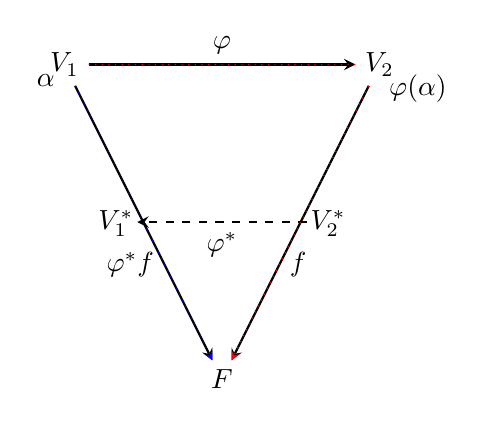
\begin{tikzpicture}[>=stealth, node distance=3cm]
            % 定义节点
            \node (V1) at (0,2) {$V_1$};
            \node (V2) at (4,2) {$V_2$};
            \node (V1s) at (0,0) {};
            \node (V2s) at (4,0) {};
            \node (F) at (2,-2) {$F$};
            
            % 绘制主要箭头
            \draw[->, thick] (V1) -- node[above] {$\varphi$} (V2);
            \draw[->, thick] (V1) -- node[left] {$V_1^*$} node[pos=0.65,left]{$\varphi^*f$}(F);
            \draw[->, thick] (V2) -- node[right] {$V_2^*$} node[pos=0.65,right]{$f$}(F);
            
            % 使用缩短的箭头绘制φ*
            \draw[->, thick, dashed, shorten >=0.8cm, shorten <=0.8cm] 
                (V2s) -- node[below] {$\varphi^*$} (V1s);
            
            % 标注α和β
            \node[below left] at (V1) {$\alpha$};
            \node[below right] at (V2) {$\varphi(\alpha)$};
            
            % 标注函数作用路径
            \draw[->, dotted, red] (V1) -- (V2) -- (F);
            \draw[->, dotted, blue] (V1) -- (F);
        \end{tikzpicture}
        
        $\varphi^*f(\alpha) = f(\varphi(\alpha))$
        \end{center}
        
        
            下面这个性质是关于有限维\线性映射 的表示矩阵的, 将其整理在这.
            \begin{ppt}
                []
                {\伴随映射 的矩阵表示为其转置}
                []
                []
                $V_1$, $V_2$均为有限维\线性空间. 设$A$为$\varphi$ 在某组基下的矩阵表示, 则$\varphi^*$在对应的\对偶基 下的矩阵表示为$A^T$.
            \end{ppt}

            \begin{prf}
                设$v_1,v_2,\cdots,v_n$为$V_1$的基, $v_1^*, v_2^*,\cdots,v_n^*$ 为\对偶基. 
                $w_1,w_2,\cdots,w_m$为$V_2$的基, $w_1^*, w_2^*,\cdots, w_m^*$为\对偶基. 
                
                设$(\varphi\circ v_1,\varphi\circ v_2,\cdots,\varphi\circ v_n)=(w_1,w_2\cdots,w_m)A$, 
                要描述一个\线性映射, 我们只需描述其在一组基上的像:
                \[(\varphi^*\circ w_1^*,\varphi^*\circ w_2^*\cdots,\varphi^*\circ w_m^*)^T\circ(v_1,v_2,\cdots,v_n)\]
                \[=(w_1^*\circ\varphi,w_2^*\circ\varphi,\cdots,w_m^*\circ\varphi)^T\circ(v_1,v_2,\cdots,v_n)\]
                \[=(w_1^*,w_2^*,\cdots,w_m^*)^T\circ(\varphi\circ v_1,\varphi\circ v_2,\cdots,\varphi\circ v_n)\]
                \[=(w_1^*,w_2^*,\cdots,w_m^*)^T\circ(w_1,w_2,\cdots,w_m)A\]
                \[=A(v_1^*,v_2^*,\cdots,v_n^*)^T\circ(v_1,v_2,\cdots,v_n)\]
                于是有$(\varphi^*\circ w_1^*,\varphi^*\circ w_2^*\cdots,\varphi^*\circ w_m^*)^T=A(v_1^*,v_2^*,\cdots,v_n^*)^T$, 
                因为他们作用在基$(v_1,v_2,\cdots,v_n)$上的效果是相同的. 即是说
                \[(\varphi^*\circ w_1^*,\varphi^*\circ w_2^*\cdots,\varphi^*\circ w_m^*)=(v_1^*,v_2^*,\cdots,v_n^*)A^T\]
                故$A^T$即为$\varphi^*$的矩阵表示
            \end{prf}
            
        
		
	
	\subsection{\线性映射 基本定理}
	下面的内容与抽象代数中的一些定理有很强的关联性,所以我们先引入一些新的概念.
		\begin{dfn}
			[]
			{核(空间)}
			[Kernel (Space)]
			[]

			设$\varphi:V_1\to V_2$是\线性映射, \线性空间$V_1$的子集$$S=\{v|v\in V_1,\varphi(v)=\mathbf{0}\}$$称为\线性映射$\varphi$的\textbf{核(Kernel)}, 记为$\ker\varphi$. 
		\end{dfn}
  
        \begin{dfn}
			[]
			{像(空间)}
			[Image (Space)]
			[]

            同样设$\varphi:V_1\to V_2$是\线性映射, 则\线性空间$V_2$的子集
            \[T=\{\varphi (w)|w\in V_1\}\]
            称为\线性映射$\varphi$的\textbf{像(空间)}, 记为$\Im\varphi$
        \end{dfn}
        \begin{ppt}
			[]
			{线性性}
			[]
			[]

            上述两个"集合"都关于其对应的加法,数乘成\线性空间.
        \end{ppt}
        \begin{prf}
            若$v,w\in \ker\varphi$, 则
            \[\varphi(v+w)=\varphi(v)+\varphi(w)=0\Longrightarrow v+w\in\ker\varphi\]
            \[\varphi(kv)=l\varphi(v)=0\Longrightarrow kv\in\ker\varphi\]
            \[\varphi(v)+\varphi(w)=\varphi(v+w)\Longrightarrow\varphi(v+w)\in\Im\varphi\]
            \[k\varphi(v)=\varphi(kv)\Longrightarrow k\varphi(v)\in\Im\varphi\]
        \end{prf}
        于是以后我们提到"\线性映射 的核"或"\线性映射 的像"是指该\线性空间 而不仅仅是向量的集合.\\
        回忆\商空间 的概念, 下面这个定理揭示了上述两个子空间的关系.
        
        \begin{thm}
			[]
			{\线性映射 基本定理 / 第一同构定理 / \商空间 同构定理}
			[Fundamental Thoerem of Linear Maps / Isomorphism Theroem A / Quotient Space Isomorphism Thoerem]
			[]

			设$\varphi:V_1\to V_2$为一个\线性映射, 则有以下同构映射$\bar{\varphi}$诱导的同构:
			\[\overline{\varphi}:V_1/\ker\varphi\cong\Im\varphi\]
			\[\overline{\alpha}\to\varphi(\alpha)\]
			\end{thm}
			\begin{prf}
			对$V_1/\ker\varphi$中的每个元素$\bar{\alpha}$, 定义映射$\bar{\varphi}$为$\bar{\varphi}(\bar{\alpha})=\varphi(\alpha)\in\Im\varphi$. 
			首先$\bar{\varphi}$一定是个满射. 对任意$\beta=\varphi(\alpha)\in\Im\varphi$, 必有$\bar{\varphi}(\bar{\alpha})=\varphi(\alpha)=\beta$. 其次他也一定是单射, 若$\bar{\varphi}(\bar{\alpha})=\bar{\varphi}(\bar{\beta})$, 则$\varphi(\alpha)-\varphi(\beta)=\varphi(\alpha-\beta)=0$, 故$\alpha-\beta\in\ker\varphi$, 即$\bar{\alpha}=\bar{\beta}$, 于是证得其为单射,故为双射.
        \end{prf}

		\begin{dfn}
			[]
			{商映射}
			[Quotient Map]
			[]

			对于\线性空间$V$及其子空间$U$,称如下的映射$\pi$
			\[\begin{bmatrix}
				V&\to&V/U\\
				v&\mapsto&v+U 
			\end{bmatrix}\]
			为\textbf{商映射}.
		\end{dfn}

		\begin{dfn}
			[]
			{\线性映射 的陪映射}
			[]
			[]

			设$T\in\Hom_{\F}(V,W)$. 规定其\textbf{陪映射}$\tilde{T}$为:
			\[\begin{bmatrix}
				V/(\Null T)&\to&W\\
				v+\Null T&\mapsto&Tv
			\end{bmatrix}\]
		\end{dfn}

		\begin{ppt}
			[]
			{陪映射的性质}
			[]
			[]

			设$T\in\Hom_{\F}(V,W)$. 陪映射为$\tilde{T}$, 则

			(1) $\tilde{T}\circ\pi=T$; ($\pi$是$V$和$\Null T$的商映射)\\
			(2) $\tilde{T}$是线性单射;\\
			(3) $\tilde{T}$与$T$有相同的像空间.
		\end{ppt}

		\begin{thm}
			[]
			{第二同构定理}
			[Isomorphism Theorem B]
			[]

			对任意的\线性子空间 $U$ 和 $V$:
			\[
			\frac{U + V}{U} \simeq \frac{V}{U \cap V}. 
			\]
		\end{thm}
		\begin{thm}
			[]
			{第三同构定理}
			[Isomorphism Theorem C]
			[]

			如果\线性空间 之间满足 $U \subset V \subset W$, 那么存在一个同构映射:
			\[
			\frac{W}{V} \simeq \frac{W / U}{V / U}.
			\]
		\end{thm}

		\begin{crl}
			[]
			{商运算与Cartesian运算具备结合律}
			[]
			[]

			设 $U_i \subset V_i$ 是\线性子空间,则
			\[
			\frac{V_1 \times V_2}{U_1 \times U_2} \simeq (U_1/V_1) \times (U_2/V_2).
			\]
		\end{crl}
        
	
	\subsection{坐标向量与基变换}
		
		\begin{thm}
			[]
			{维度与空间的对应关系}
			[]
			[]

			设$V$是\数域$\K$上的\线性空间, 则$\dim V=n\Longrightarrow V\cong\K_n$
		\end{thm}
  
		\begin{prf}
			选取$V$的一组基$E=\{e_1,e_2,\cdots,e_n\}$, 
			
			$$\forall v\in V, \exists k_1,k_2,\cdots,k_n\in\K:v=\sum_{i=1}^nk_ie_i$$
			
			$\because E$线性无关, $\Longrightarrow$这样的表示唯一, 可构造$\eta:V\to\K_n: \eta(v)=\begin{bmatrix}k_1\\k_2\\\vdots\\k_n\end{bmatrix}$, 
			
			$$\forall k_1,k_2,\cdots,k_n, \eta^{-1}(\begin{bmatrix}k_1\\k_2\\\vdots\\k_n\end{bmatrix})=\sum_{i=1}^nk_ie_i$$
			
			有$\eta$是双射, 又显然$\eta$为\线性映射, 即有$V\cong K_n$. $\square$
		\end{prf}
  
		\begin{thm}
			[]
			{维度与空间的对应性}
			[]
			[]

			设\线性映射$\varphi:V_1\to V_2, \dim V_1=m, \dim V_2=n$, 可绘制如下交换图: 
			$$\begin{matrix}
			\xymatrix{
			V_1\ar[r]^\varphi\ar[d]^{\eta_1} & V_2\ar[d]^{\eta_2}\\
			\K_m\ar[r]^{\varphi^*}\ar[u] & \K_n\ar[u]
			}
			\end{matrix}$$
		\end{thm}

	\subsection{不变子空间}
		\begin{dfn}
			[]
			{不变子空间}
			[Invariant Subspace]
			[]

			设$\varphi$是$V$上的线性变换,$W$是$V$的子空间,如果$W$中的向量在$\varphi$的像仍在$W$中,就称$W$是$\varphi$的\textbf{不变子空间}。
		\end{dfn}

		\begin{ppt}
			[]
			{几种特殊的不变子空间}
			[]
			[]

			\begin{itemize}
				\item 全空间$V$与零子空间$\0$是所有线性变换的不变子空间。
				\item $\varphi$的像空间与核空间都是它的不变子空间。
				\item 假如存在与$\varphi$可交换的线性变换$\psi$, 那么$\psi$的像空间与核空间都是$\varphi$的不变子空间。
			\end{itemize}
		\end{ppt}
	
\section{矩阵}
	
	\subsection{\线性映射 与矩阵}
		\begin{thm}
			[]
			{两个\线性映射 的关系的表示}
			[]
			[]

			设\线性映射$\varphi:\K_m\to \K_n$, 则: 
			
			$$\exists a_{1,1},a_{1,2},\cdots a_{m,n}\in\K: $$
			
			$$\forall v=\begin{bmatrix}b_1\\b_2\\\vdots\\b_m\end{bmatrix}\in V_1, \varphi(v)=\begin{bmatrix}c_1\\c_2\\\vdots\\c_n\end{bmatrix}\in V_2, $$
			
			$$c_j=\sum_{i=1}^{m}a_{i,j}b_i$$
		\end{thm}
  
		\begin{prf}
			考虑$e_i,f_j=\begin{bmatrix}0\\\vdots\\1\\\vdots\\0\end{bmatrix}(1\leq i\leq m, 1\leq j\leq n)$(第$i$或$j$行为$1$, 其余全部为0), 有: 
			
			$$v=\sum_{i=1}^{m}b_{i}e_i, \varphi(v)=\sum_{j=1}^{m}c_{j}f_j$$
			
			$$\mbox{设}\varphi(e_i)=\sum_{j=1}^{m}a_{i,j}f_j\mbox{, 则有: }$$
			
			$$\varphi(v)=\sum_{i=1}^{m}b_{i}\varphi(e_i)=\sum_{i=1}^{m}(b_{i}\sum_{j=1}^{m}a_{i,j}f_j)=\sum_{j=1}^{m}(\sum_{i=1}^{n}a_{i,j}b_i)f_j$$
			
			又$\because\{f_1,f_2,\cdots,f_n\}$线性无关, 即$\varphi(v)$的表示方式唯一, 
			
			$$\Longrightarrow c_j=\sum_{i=1}^{n}a_{i,j}b_i\square$$
		\end{prf}
  
		\begin{dfn}
			[]
			{矩阵}
			[]
			[]

			线性映射$\varphi:\K_m\to \K_n$可由$a_{1,1},a_{1,2},\cdots a_{m,n}\in\K$唯一确定. 将这$m\times n$个数写成一个矩形阵列, 称为\textbf{矩阵(Matrix)}, 写作: 
			$$\begin{bmatrix}
				a_{1,1}&a_{1,2}&\cdots&a_{1,n}\\
				a_{2,1}&a_{1,2}&\cdots&a_{1,n}\\
				\vdots&\vdots&\ddots&\vdots\\
				a_{m,1}&a_{m,2}&\cdots&a_{m,n}
			\end{bmatrix}$$
			简写作$(a_{i,j})_{m\times n}$. 
		\end{dfn}
		
		\begin{dfn}
			[]
			{矩阵的四个基本子空间}
			[]
			[]

			矩阵$A$各行向量组\张成 的\线性空间 称为矩阵$A$的\textbf{行空间(Row Space)}, 记作$\RRow A$, 也记作$\Im A^T$, 行空间是矩阵对应线性映射的定义域; 
			
			矩阵$A$各列向量组\张成 的\线性空间 称为矩阵$A$的\textbf{列空间(Column Space)}, 记作$\CCol A$, 也记作$\Im A$, 列空间是矩阵对应线性映射的值域; 

			满足$Av=\mathbf{0}$的全体向量$v$组成矩阵$A$的\textbf{零空间}, 记作$\Null A$, 零空间是矩阵对应线性映射的核; 

			满足$A^T u=\mathbf{0}$的全体向量$u$组成矩阵$A$的\textbf{左零空间}, 记作$\Null A^T$
		\end{dfn}
	
	\subsection{矩阵的运算}
		\begin{dfn}
			[]
			{矩阵的积}
			[]
			[]

			设矩阵$A$和$B$分别为线性映射$\varphi_A: V_2\to V_3$与$\varphi_B:V_1\to V_2$在$V_1,V_2,V_3$的一组基下的表示矩阵, $A$与$B$的\textbf{积(Product)}定义为线性映射$\varphi_A\circ\varphi_B$在这组基下的表示矩阵, 记为$A\cdot B$或简写为$AB$. 
		\end{dfn}
		
		\begin{thm}
			[]
			{矩阵的积的运算法}
			[]
			[]

			设$A=(a_{i,p})_{m\times k}, B=(b_{p,j})_{k\times n}$, 则:
			
			$$AB=(\sum_{p=1}^{k}a_{i,p}b_{p,j})_{m\times n}$$
		\end{thm}
		\begin{prf}
		证明: 
			
			设$\alpha=\begin{bmatrix}x_1\\x_2\\\vdots\\x_n\end{bmatrix}$, 则$B\alpha=
			\begin{bmatrix}
				b_{1,1}&b_{1,2}&\cdots&b_{1,n}\\
				b_{2,1}&b_{1,2}&\cdots&b_{1,n}\\
				\vdots&\vdots&\ddots&\vdots\\
				b_{k,1}&b_{k,2}&\cdots&b_{k,n}
			\end{bmatrix}
			\begin{bmatrix}
			x_1\\x_2\\\vdots\\x_n
			\end{bmatrix}=
			\begin{bmatrix}
			\sum_{j=1}^{n}b_{1,j}x_j\\\sum_{j=1}^{n}b_{2,j}x_j\\\vdots\\\sum_{j=1}^{n}b_{k,j}x_j
			\end{bmatrix}$
			
			$$AB\alpha=
			\begin{bmatrix}
				a_{1,1}&a_{1,2}&\cdots&a_{1,k}\\
				a_{2,1}&a_{1,2}&\cdots&a_{1,k}\\
				\vdots&\vdots&\ddots&\vdots\\
				a_{m,1}&a_{m,2}&\cdots&a_{m,k}
			\end{bmatrix}
			\begin{bmatrix}
			\sum_{j=1}^{n}b_{1,j}x_j\\\sum_{j=1}^{n}b_{2,j}x_j\\\vdots\\\sum_{j=1}^{n}b_{k,j}x_j
			\end{bmatrix}$$
			
			$$
			=\begin{bmatrix}
			\sum_{p=1}^{k}a_{1,p}(\sum_{j=1}^{n}b_{p,j}x_j)\\
			\sum_{p=1}^{k}a_{2,p}(\sum_{j=1}^{n}b_{p,j}x_j)\\
			\vdots\\
			\sum_{p=1}^{k}a_{m,p}(\sum_{j=1}^{n}b_{p,j}x_j)
			\end{bmatrix}
			=\begin{bmatrix}
			\sum_{j=1}^{n}[\sum_{p=1}^{k}(a_{1,p}b_{p,j})x_j]\\
			\sum_{j=1}^{n}[\sum_{p=1}^{k}(a_{2,p}b_{p,j})x_j]\\
			\vdots\\
			\sum_{j=1}^{n}[\sum_{p=1}^{k}(a_{m,p}b_{p,j})x_j]
			\end{bmatrix}$$
			
			$$
			=(\sum_{p=1}^{k}a_{i,p}b_{p,j})_{m\times n}\begin{bmatrix}x_1\\x_2\\\vdots\\x_n\end{bmatrix}
			$$
			
			$$\Longrightarrow AB=(\sum_{p=1}^{k}a_{i,p}b_{p,j})_{m\times n}\square$$
		\end{prf}
  
		\begin{ppt}
			[]
			{矩阵乘法满足结合律}
			[]
			[]
			
			设$A,B,C$分别为$m\times k, k\times l, l\times n$矩阵, 则$A(BC)=(AB)C$, 记作$ABC$. 
		\end{ppt}
  
		\begin{prf}
			考虑$A,B,C$对应的线性映射: 
			
			$$\varphi_A:\K_k\to\K_m,\varphi_B:\K_l\to\K_k,\varphi_C:\K_n\to\K_l$$
			
			$$\because\varphi_A\circ(\varphi_B\circ\varphi_C)=(\varphi_A\circ\varphi_B)\circ\varphi_C$$
			
			$\Longrightarrow (AB)C=A(BC)$对应的线性映射均为$\varphi_A\circ\varphi_B\circ\varphi_C.\square$
		\end{prf}
  
		\begin{dfn}
			[]
			{转置}
			[]
			[]

			矩阵$A=(a_{i,j})_{m\times n}$的\textbf{转置(Transpose)}定义为$A'=(a_{j,i})_{n\times m}$, 记为$A^T$. 
		\end{dfn}
		
		\begin{ppt}
			[]
			{矩阵乘法的转置满足反交换律}
			[]
			[]
			
			$$(AB)^T=B^TA^T$$
		\end{ppt}
  
		\begin{prf}
		
			设$A=(a_{i,p})_{m\times k}, B=(b_{p,j})_{k\times n}$, 则: 
			
			$$A^T=(a_{p,i})_{k\times m}, B^T=(b_{j,p})_{n\times k}$$
			
			$$AB=(\sum_{p=1}^{k}a_{i,p}b_{p,j})_{m\times n}$$
			
			$$(AB)^T=(\sum_{p=1}^{k}a_{j,p}b_{p,i})_{n\times m}=B^TA^T\square$$
		\end{prf}

		\begin{dfn}
			[]
			{几种特殊的矩阵}
			[]
			[]

			矩阵$(a_{i,j})_{n\times n}$称为$n$阶\textbf{方阵(Square Matrix)}, 记为$(a_{i,j})_n$. 
			
			方阵$(a_{i,j})_n$称为是一个\textbf{上三角阵(Upper Triangular Matrix)}, 若: $$\forall j>i, a_{i,j}=0$$
			
			方阵$(a_{i,j})_n$称为是一个\textbf{下三角阵(Lower Triangular Matrix)}, 若: $$\forall i>j, a_{i,j}=0$$
			
			方阵$(a_{i,j})_n$称为是一个\textbf{对角阵(Diagonal Matrix)}, 若$\forall i\neq j, a_{i,j}=0$, 记为${\rm diag}\{a_{1,1},a_{2,2},\cdots,a_{n,n}\}$. 
			
			恒同映射$\Id:\K_n\to\K_n$对应的矩阵称为n阶\textbf{单位阵(Identity Matrix)}, 记作$I_n$. 
		\end{dfn}
		
		\begin{ppt}
			[]
			{单位矩阵}
			[]
			[]

			$I_n={\rm diag}\{\underbrace{1,1,\cdots,1}_{n\mbox{个}1}\}$
		\end{ppt}
		
		\begin{ppt}
			[]
			{单位矩阵的交换性}
			[]
			[]

			$\forall m\times n$矩阵$A$, $AI_n=I_mA=A$
		\end{ppt}

        \begin{prf}
			 考虑$A,I_n$对应的线性变换$\varphi_A,\Id$, 有$\varphi_A\circ \Id=\Id\circ\varphi_A=\varphi_A$. 
			
			 考虑等式每一项对应的矩阵, 即有$AI_n=I_mA=A$. $\square$
		\end{prf}
  
		\begin{ppt}
			[]
			{三角矩阵对积运算的封闭性}
			[]
			[]

			同阶上三角阵之积为上三角阵, 同阶下三角阵之积为下三角阵. 
		\end{ppt}
		
		
		
	\subsection{方阵的逆阵}
		
		\begin{dfn}
			[]
			{可逆矩阵}
			[]
			[]

			$n$阶方阵$A$称为一个\textbf{可逆阵(Invertible)}或\textbf{非奇异阵(Non-Singular Matrix)}, 若$\exists n$阶方阵$A': AA'=A'A=I_n$; 否则称为\textbf{奇异阵(Singular Matrix)}. 
		\end{dfn}
		
		\begin{dfn}
			[]
			{逆矩阵}
			[]
			[]

			$n$阶方阵$A'$称为$n$阶可逆阵$A$的\textbf{逆阵(Inverse)}, 若$AA'=A'A=I_n$, 记作$A^{-1}$. 
		\end{dfn}
		
		\begin{ppt}
			[]
			{逆阵唯一}
			[]
			[]
		
			$\forall n$阶方阵$A$, 至多$\exists$一个$n$阶方阵$A'$满足$AA'=A'A=I_n$. 
		\end{ppt}

        \begin{prf}
			设对某个$n$阶方阵$A, \exists A',A'': AA'=A'A=AA''=A''A=I_n$. 
			
			$$\Longrightarrow A'=A'I_n=A'(AA'')=(A'A)A''=I_nA''=A''\square$$
	    \end{prf}
 
		\begin{ppt}
			[]
			{逆运算与积运算的反交换性}
			[]
			[]

			可逆阵之积仍为可逆阵, 且运算满足反交换律: 
			
			设$A,B$是$n$阶可逆阵, $(AB)^{-1}=B^{-1}A^{-1}$
		\end{ppt}
  
		\begin{prf}
            $B^{-1}A^{-1}AB=B^{-1}B=I_n$, 同理$ABB^{-1}A^{-1}=I_n$, 即$(AB)^{-1}=B^{-1}A^{-1}\square$
		\end{prf}
		
		
		\begin{ppt}
			[]
			{一般线性群}
			[]
			[]

			\数域$\K$上的$n$阶可逆阵全体在矩阵乘法运算下构成一个群, 称为\数域$\K$上的$n$阶\textbf{一般线性群(General Linear Group)}, 记为$GL_n(\K)$
		\end{ppt}
  
		\begin{prf}
			 $n$阶可逆阵全体关于矩阵乘法封闭, 矩阵乘法满足结合律, 恒等元为$I_n$, 任意$n$阶可逆阵$A$的逆元为$A^{-1}$
			
			$\Longrightarrow n$阶可逆阵全体在矩阵乘法运算下构成一个群. $\square$
        \end{prf}
        
		\begin{dfn}
			[]
			{相似关系}
			[]
			[]
  
            我们称矩阵$A$,$B$相似,当且仅当存在可逆矩阵$P$,使得
            \[P^{-1}AP=B\]

		\end{dfn}
		
		\begin{dfn}
			[]
			{迹(Trace)}
			[]
			[]

            方阵$A$的主对角线上的元素之和称为迹,记作$tr(A)$
		\end{dfn}
		
	\subsection{矩阵的初等变换与Gauss消元法}
	
		\begin{dfn}
			[]
			{初等线性变换}
			[]
			[]

			设$\{e_1,e_2,\cdots,e_n\}$是\数域$\K$上$n$维线性空间$V$的一组基, 则以下三类线性变换称为\textbf{初等线性变换(Elementary Linear Transformation)}, 简称为\textbf{初等变换(Elementary Transformation)}: 
			
			第一类初等变换: $$\varphi(e_i)=e_j, \varphi(e_j)=e_i, \varphi(e_p)=e_p(\forall p\neq i,j)$$
			
			第二类初等变换: $$\varphi(e_i)=ke_i, \varphi(e_p)=e_p(\forall p\neq i, \forall k\in(\K-\{0\}))$$
			
			第三类初等变换: $$\varphi(e_i)=e_i+ke_j, \varphi(e_p)=e_p(\forall p\neq i, \forall k\in\K)$$
			
			将恒同变换$\Id$视为特殊的初等变换. 
		\end{dfn}
		
		\begin{ppt}
			[]
			{线性自同构的初等性}
			[]
			[]

			$\forall$有限维线性空间$V$上的线性自同构$\varphi$, $\varphi$可表示为有限个初等线性变换的复合. 
		\end{ppt}
  
		\begin{prf}
			设$E=\{e_1,e_2,\cdots,e_n\}$是$V$的一组基, 则$\varphi(E)=\{\varphi(e_1),\varphi(e_2),\cdots,\varphi(e_n)\}$是$V$的一组基. 
			
			$\varphi(e_1)$可被$E$唯一线性表示, 设$\varphi(e_1)=\sum_{i=1}^{n}k_{i}e_i$, 其中$k_i$不全为$0$. 
			
			设$k_i\neq 0$. 先对$V$作第二类初等变换: $\varphi_1(e_i)=k_ie_i, \varphi_1(e_p)=e_p(\forall p\neq i)$
			
			再对$V$作$n-1$次第三类初等变换: $\varphi_2(k_ie_i)=k_ie_i+k_1e_1$,
			
			$$\varphi_3(k_ie_i+k_1e_1)=k_ie_i+k_1e_1+k_2e_2, \cdots, $$
			
			$$\varphi_n(k_ie_i+\sum_{p\neq i,n}k_pe_p)=k_ie_i+\sum_{p\neq i}k_pe_p=\varphi(e_1)$$
			
			$$\Longrightarrow \varphi_n\circ\varphi_{n-1}\circ\cdots\circ\varphi_1(E)=\{\varphi(e_1),e_2,e_3,\cdots,e_n\}$$
			
			再对$e_2,e_3,\cdots,e_n$执行同样的变换即将$E$变换为$\varphi(E)$. 
			
			即$\varphi$可由有限个初等变换复合得到. $\square$
		\end{prf}
		
		\begin{dfn}
			[]
			{初等矩阵}
			[]
			[]

			上述三类初等线性变换对应的方阵称为\textbf{初等矩阵(Elementary Matrix)}. 将单位阵$I_n$视为特殊的初等矩阵. 
		\end{dfn}
		
		\begin{ppt}
			[]
			{三类初等矩阵}
			[]
			[]

			三类$n$阶初等矩阵的形式分别为: 
			
			第一类初等矩阵: 
			
			$$\begin{bmatrix}
			1 & & & & & & 0\\
			 &\ddots & & & & & \\
			 & & 0 & \cdots & 1 & & \\
			 & &\vdots &\ddots &\vdots & & \\
			 & & 1 & \cdots & 0 & & \\
			 & & & & &\ddots & \\
			0 & & & & & & 1\\
			\end{bmatrix}$$
			
			($a_{i,i}=a_{j,j}=0,a_{i,j}=a_{j,i}=1,$ 其余与$I_n$相同)
			
			第二类初等矩阵: 
			
			$$\begin{bmatrix}
			1 & & & & & & 0\\
			 &\ddots & & & & & \\
			 & & 1 & & & & \\
			 & & & k & & & \\
			 & & & & 1 & & \\
			 & & & & & \ddots & \\
			0 & & & & & & 1\\
			\end{bmatrix}$$
			
			(${\rm diag}\{1,\cdots,1,k,1,\cdots,1\}, a_{i,i}=k$, 其余与$I_n$相同)
			
			第三类初等矩阵: 
			
			$\begin{bmatrix}
			1 & & & & & & 0\\
			 &\ddots & & & & & \\
			 & & 1 & & & & \\
			 & &\vdots &\ddots & & & \\
			 & & k & \cdots & 1 & & \\
			 & & & & &\ddots & \\
			0 & & & & & & 1\\
			\end{bmatrix}$
			或
			$\begin{bmatrix}
			1 & & & & & & 0\\
			 &\ddots & & & & & \\
			 & & 1 & \cdots & k & & \\
			 & & &\ddots & \vdots & & \\
			 & & & & 1 & & \\
			 & & & & &\ddots & \\
			0 & & & & & & 1\\
			\end{bmatrix}$
			
			($a_{j,i}=k$, 其余与$I_n$相同)
		\end{ppt}
		
		\begin{ppt}
			[]
			{初等矩阵的可逆性}
			[]
			[]

			初等矩阵都是可逆阵, 且其逆阵为初等矩阵. 
		\end{ppt}
  
		\begin{prf}	
			(1)$$\begin{bmatrix}
			1 & & & & & & 0\\
			 &\ddots & & & & & \\
			 & & 0 & \cdots & 1 & & \\
			 & &\vdots &\ddots &\vdots & & \\
			 & & 1 & \cdots & 0 & & \\
			 & & & & &\ddots & \\
			0 & & & & & & 1\\
			\end{bmatrix}^2=I_n$$
			
			(2)$$\begin{bmatrix}
			1 & & & & & & 0\\
			 &\ddots & & & & & \\
			 & & 1 & & & & \\
			 & & & k & & & \\
			 & & & & 1 & & \\
			 & & & & & \ddots & \\
			0 & & & & & & 1\\
			\end{bmatrix}
			\begin{bmatrix}
			1 & & & & & & 0\\
			 &\ddots & & & & & \\
			 & & 1 & & & & \\
			 & & & \frac{1}{k} & & & \\
			 & & & & 1 & & \\
			 & & & & & \ddots & \\
			0 & & & & & & 1\\
			\end{bmatrix}=I_n$$
			
			(3)$$\begin{bmatrix}
			1 & & & & & & 0\\
			 &\ddots & & & & & \\
			 & & 1 & & & & \\
			 & &\vdots &\ddots & & & \\
			 & & k & \cdots & 1 & & \\
			 & & & & &\ddots & \\
			0 & & & & & & 1\\
			\end{bmatrix}
			\begin{bmatrix}
			1 & & & & & & 0\\
			 &\ddots & & & & & \\
			 & & 1 & & & & \\
			 & &\vdots &\ddots & & & \\
			 & & -k & \cdots & 1 & & \\
			 & & & & &\ddots & \\
			0 & & & & & & 1\\
			\end{bmatrix}=I_n\square$$
		\end{prf}
		
		\begin{dfn}
			[]
			{初等变换}
			[]
			[]

			以下三类对矩阵$(a_{i,j})_{m\times n}$进行的变换称为矩阵的三类\textbf{初等行变换(Elementary Row Transformation)}: 
			
			(1)第一类初等行变换: 
			
			\[\begin{gmatrix}[b]
			a_{1,1} & a_{1,2} & \cdots & a_{1,n}\\
			\vdots & \vdots & \ddots & \vdots \\
			a_{i,1} & a_{i,2} & \cdots & a_{i,n} \\
			\vdots & \vdots & \ddots & \vdots \\
			a_{j,1} & a_{j,2} & \cdots & a_{j,n}\\
			\vdots & \vdots & \ddots & \vdots \\
			a_{m,1} & a_{m,2} & \cdots & a_{m,n}
			\rowops
			\swap{2}{4}
			\end{gmatrix}\longrightarrow
			\begin{gmatrix}[b]
			a_{1,1} & a_{1,2} & \cdots & a_{1,n}\\
			\vdots & \vdots & \ddots & \vdots \\
			a_{j,1} & a_{j,2} & \cdots & a_{j,n} \\
			\vdots & \vdots & \ddots & \vdots \\
			a_{i,1} & a_{i,2} & \cdots & a_{i,n}\\
			\vdots & \vdots & \ddots & \vdots \\
			a_{m,1} & a_{m,2} & \cdots & a_{m,n}
			\end{gmatrix}\]
			
			(2)第二类初等行变换: 
			
			\[\begin{gmatrix}[b]
			a_{1,1} & a_{1,2} & \cdots & a_{1,n}\\
			\vdots & \vdots & \ddots & \vdots \\
			a_{i,1} & a_{i,2} & \cdots & a_{i,n} \\
			\vdots & \vdots & \ddots & \vdots \\
			a_{m,1} & a_{m,2} & \cdots & a_{m,n}
			\rowops
			\mult{2}{k}
			\end{gmatrix}\longrightarrow
			\begin{gmatrix}[b]
			a_{1,1} & a_{1,2} & \cdots & a_{1,n}\\
			\vdots & \vdots & \ddots & \vdots \\
			ka_{i,1} & ka_{i,2} & \cdots & ka_{i,n} \\
			\vdots & \vdots & \ddots & \vdots \\
			a_{m,1} & a_{m,2} & \cdots & a_{m,n}
			\end{gmatrix}\]
			
			(3)第三类初等行变换: 
			
			\[\begin{gmatrix}[b]
			a_{1,1} & a_{1,2} & \cdots & a_{1,n}\\
			\vdots & \vdots & \ddots & \vdots \\
			a_{i,1} & a_{i,2} & \cdots & a_{i,n} \\
			\vdots & \vdots & \ddots & \vdots \\
			a_{j,1} & a_{j,2} & \cdots & a_{j,n}\\
			\vdots & \vdots & \ddots & \vdots \\
			a_{m,1} & a_{m,2} & \cdots & a_{m,n}
			\rowops
			\add[k]{2}{4}
			\end{gmatrix}\longrightarrow
			\begin{gmatrix}[b]
			a_{1,1} & a_{1,2} & \cdots & a_{1,n}\\
			\vdots & \vdots & \ddots & \vdots \\
			a_{i,1} & a_{i,2} & \cdots & a_{i,n} \\
			\vdots & \vdots & \ddots & \vdots \\
			a_{j,1}+ka_{i,1} & a_{j,2}+ka_{i,2} & \cdots & a_{j,n}+ka_{i,n}\\
			\vdots & \vdots & \ddots & \vdots \\
			a_{m,1} & a_{m,2} & \cdots & a_{m,n}
			\end{gmatrix}\]
			
			以下三类对矩阵$(a_{i,j})_{m\times n}$进行的变换称为矩阵的三类\textbf{初等列变换(Elementary Column Transformation)}: 
			
			(1')第一类初等列变换: 
			\[\begin{gmatrix}[b]
			a_{1,1} & \cdots & a_{1,i} & \cdots & a_{1,j} & \cdots & a_{1,n}\\
			a_{2,1} & \cdots & a_{2,i} & \cdots & a_{2,j} & \cdots & a_{2,n} \\
			\vdots & \ddots & \vdots & \ddots & \vdots & \ddots & \vdots \\
			a_{m,1} & \cdots & a_{m,i} & \cdots & a_{m,j} & \cdots & a_{m,n}
			\colops
			\swap{2}{4}
			\end{gmatrix}\]
			
			\[\longrightarrow
			\begin{gmatrix}[b]
			a_{1,1} & \cdots & a_{1,j} & \cdots & a_{1,i} & \cdots & a_{1,n}\\
			a_{2,1} & \cdots & a_{2,j} & \cdots & a_{2,i} & \cdots & a_{2,n} \\
			\vdots & \ddots & \vdots & \ddots & \vdots & \ddots & \vdots \\
			a_{m,1} & \cdots & a_{m,j} & \cdots & a_{m,i} & \cdots & a_{m,n}
			\end{gmatrix}\]
			
			(2')第二类初等列变换: 
			\[\begin{gmatrix}[b]
			a_{1,1} & \cdots & a_{1,i} & \cdots & a_{1,n}\\
			a_{2,1} & \cdots & a_{2,i} & \cdots & a_{2,n} \\
			\vdots & \ddots & \vdots & \ddots & \vdots \\
			a_{m,1} & \cdots & a_{m,i} & \cdots & a_{m,n}
			\colops
			\mult{2}{k}
			\end{gmatrix}\]
			
			\[\longrightarrow
			\begin{gmatrix}[b]
			a_{1,1} & \cdots & ka_{1,i} & \cdots & a_{1,n}\\
			a_{2,1} & \cdots & ka_{2,i} & \cdots & a_{2,n} \\
			\vdots & \ddots & \vdots & \ddots & \vdots \\
			a_{m,1} & \cdots & ka_{m,i} & \cdots & a_{m,n}
			\end{gmatrix}\]
			
			(3')第三类初等列变换: 
			\[\begin{gmatrix}[b]
			a_{1,1} & \cdots & a_{1,i} & \cdots & a_{1,j} & \cdots & a_{1,n}\\
			a_{2,1} & \cdots & a_{2,i} & \cdots & a_{2,j} & \cdots & a_{2,n} \\
			\vdots & \ddots & \vdots & \ddots & \vdots & \ddots & \vdots \\
			a_{m,1} & \cdots & a_{m,i} & \cdots & a_{m,j} & \cdots & a_{m,n}
			\colops
			\add[k]{2}{4}
			\end{gmatrix}\]
			
			\[\longrightarrow
			\begin{gmatrix}[b]
			a_{1,1} & \cdots & a_{1,i} & \cdots & a_{1,j}+ka_{1,i} & \cdots & a_{1,n}\\
			a_{2,1} & \cdots & a_{2,i} & \cdots & a_{2,j}+ka_{2,i} & \cdots & a_{2,n} \\
			\vdots & \ddots & \vdots & \ddots & \vdots & \ddots & \vdots \\
			a_{m,1} & \cdots & a_{m,i} & \cdots & a_{m,j}+ka_{m,i} & \cdots & a_{m,n}
			\end{gmatrix}\]
		\end{dfn}
		
		\begin{ppt}
			[]
			{初等变换与初等矩阵的对应性}
			[]
			[]

			矩阵的三类初等行变换等价于对矩阵左乘对应的三类初等矩阵, 三类初等列变换等价于对矩阵右乘对应的三类初等矩阵. 
		\end{ppt}

        \begin{prf}
			根据矩阵乘法定义验证即可. $\square$
	    \end{prf}
 
	\subsection{矩阵的相抵关系与矩阵的\秩}
	
		\begin{dfn}
			[]
			{相抵关系}
			[]
			[]

			矩阵$A$与$B$称为满足\textbf{相抵}关系, 若$A$通过有限次初等变换后可变为$B$, 记作$A\sim B$. 
		\end{dfn}
		
		\begin{ppt}
			[]
			{相抵关系是等价关系}
			[]
			[]

		\end{ppt}
  
		\begin{prf}
			(1)自反性: 
				\[\forall A=(a_{i,j})_{m\times n}, A=AI_m=I_nA\Longrightarrow A\sim A\]
			
			(2)互逆性: 
				\[A\sim B\Longrightarrow\exists P_1,P_2,\cdots, P_q\text{($P_i$是初等矩阵)}\]
				\[B=(\prod_{i=1}^{p}P_i)A\prod_{i=p+1}^qP_{i}\]
				\[A=(\prod_{i=1}^{p}P_i^{-1})B\prod_{i=p+1}^qP_{i}^{-1}\]
				
				$P_i^{-1}$是初等矩阵$\Longrightarrow B\sim A$. 
				
			(3)传递性: 
				\[A\sim B, B\sim C\Longrightarrow\exists P_1,P_2,\cdots,P_q;P_1',P_2',\cdots,P_{q'}'\textbf{($P_i,P_i'$是初等矩阵)}\] 
				\[B=(\prod_{i=1}^{p}P_i)A\prod_{i=p+1}^qP_{i}, C=(\prod_{i=1}^{p'}P_i')B\prod_{i=p'+1}^{q'}P_i'\]
				
				\[\Longrightarrow C=(\prod_{i=1}^{p'}P_i')(\prod_{i=1}^{p}P_i)A(
                \prod_{i=p+1}^qP_{i})\prod_{i=p'+1}^{q'}P_i'\Longrightarrow A\sim C\square\]
		\end{prf}
  
		\begin{dfn}
			[]
			{行\秩 与列\秩}
			[]
			[]

			矩阵的行向量组的\秩 称为\textbf{行秩}, 列向量组的\秩 称为\textbf{列\秩}. 
		\end{dfn}
		
		\begin{ppt}
			[]
			{维度与\秩 的关系}
			[]
			[]

			矩阵行空间维数等于行\秩, 列空间维数等于列\秩. 
		\end{ppt}
  
		\begin{prf}
			{}
			{矩阵子空间的基}
			{}
			{}

			取矩阵行向量组的\极大线性无关组, 它是行空间的一组基. 
			
			对矩阵的列同理. $\square$
		\end{prf}
  
		\begin{ppt}
			[]
			{初等变换不改变行\秩 与列\秩}
			[]
			[]

			矩阵的行\秩 与列\秩 在初等变换下不变. 
		\end{ppt}
		
		\begin{dfn}
			[]
			{相抵标准形}
			[]
			[]

			若矩阵$A\sim B=
			\begin{bmatrix}
			I & O \\
			O & O 
			\end{bmatrix}$, $B$称为矩阵$A$的\textbf{相抵标准形}. 
			
			(允许其中的零矩阵$O$行数或列数为$0$. )
		\end{dfn}
		
		\begin{ppt}
			[]
			{相抵标准形的唯一性}
			[]
			[]

			任何矩阵相抵于唯一的相抵标准型. 
		\end{ppt}
  
		\begin{prf}
			运用数学归纳法. 
			
			(1)对于$1$阶矩阵$[a_{1,1}]$, 
			
			1'若$a_{1,1}=0$, $[0]$已经是相抵标准型形式. 
			
			且由于$[a_{1,1}]$的行\秩 为0, 它不相抵于$I_1$. 
			
			2'若$a_{1,1}\neq 0$,对$[a_{1,1}]$作第二类初等变换, 即有$[a_{1,1}]|\frac{1}{a_{1,1}}\longrightarrow[1]=I_1. $
			
			且由于$[a_{1,1}]$的行\秩 为1, 它不相抵于$[0]$. 
			
			(2)假设一切$k$阶矩阵均相抵于唯一相抵标准型$B$, 则利用分块矩阵的方法(打洞)将其化为分块对角阵可以很快证明
		\end{prf}
  
		\begin{thm}
			[]
			{\秩 的等价性}
			[]
			[]

			矩阵的行\秩 等于列\秩 等于矩阵的\秩. 
		\end{thm}
  
        \begin{thm}
			[]
			{满\秩}
			[]
			[]

            方阵$A$可逆当且仅当满\秩(即\秩 等于阶数)当且仅当方程$Ax=0$没有非零解
        \end{thm}
        
        \begin{prf}
            1.若$A$可逆,则当$Ax=0$时,两侧同乘$A$的逆,则有$x$为零向量,则$Ax=0$无非零解\\
            2.若$Ax=0$无非零解,也即不存在$A$的列向量的一个\线性组合 为零向量,故$A$满\秩\\
            3.若$A$满\秩,则$A$相抵于单位阵,显然可逆
        \end{prf}
        
	    \begin{ppt}
			[]
			{可逆矩阵不改变\秩}
			[]
			[]

            对矩阵进行"乘一个可逆矩阵"的操作不改变矩阵的\秩
        \end{ppt}
        \begin{prf}
            这是显然的,考虑其相抵标准型即得出该结论
        \end{prf}
        通过构造分块矩阵和上述结论,我们可以通过一些操作来证明下面这些\秩 不等式
        \begin{thm}
			[]
			{矩阵乘积的\秩}
			[]
			[]

            $r(AB)\leq \min\{r(A),r(B)\}$
        \end{thm}
        \begin{thm}
			[]
			{矩阵和的\秩}
			[]
			[]

            $r(A + B) \leq r\begin{pmatrix} A \\ B \\ \end{pmatrix} \leq r(A) + r(B)$
        \end{thm}

        \begin{thm}
			[]
			{Sylvester不等式}
			[]
			[]
        
            若$A$为$m\times p$矩阵,$B$为$p\times n$矩阵,则有
            \[r(A)+r(B)-p\leq r(AB)\]
        \end{thm}
	\subsection{适定、欠定线性方程组的解}

		考虑齐次线性方程组$\bm{A}\bm{x}=\mathbf{0}$, 其中$\bm{A}$是一个$m$行$n$列的矩阵

		容易验证这个齐次线性方程组的解是一个线性空间, 即矩阵$\bm{A}$的零空间$\Null\bm{A}$. 

		设$\rank\bm{A}=r$, 则经过适当的列交换与初等行变换后, 有: (列交换需要改变解中各个元的顺序)
		\[\bm{A}\sim\mathbf{B}:=
		\begin{bmatrix}
			1 & 0 & \cdots & 0 & c_{1,r+1} & \cdots & c_{1,n}\\
			0 & 1 & \cdots & 0 & c_{2,r+1} & \cdots & c_{2,n}\\
			\vdots & \vdots & \ddots & \vdots & \vdots & \ddots & \vdots\\
			0 & 0 & \cdots & 1 & c_{r,r+1} & \cdots & c_{r,n}\\
			0 & 0 & \cdots & 0 & 0 & \cdots & 0\\
			\vdots & \vdots & \ddots & \vdots & \vdots & \ddots & \vdots\\
			0 & 0 & \cdots & 0 & 0 & \cdots & 0\\
		\end{bmatrix}
		=
		\begin{bmatrix}
			I_d & \mathbf{C}\\
			\mathbf{O} & \mathbf{O}
		\end{bmatrix}\]

		注意到: 
		\[\begin{bmatrix}
			I_d & \mathbf{C}\\
			\mathbf{O} & \mathbf{O}
		\end{bmatrix}
		\begin{bmatrix}
			\mathbf{C}\\
			-I_d
		\end{bmatrix}=\mathbf{O}\]

		其中$\begin{bmatrix}
			\mathbf{C}\\
			-I_d
		\end{bmatrix}=\mathbf{O}$是一个列满秩阵. 

		则$\bm{B}$的零空间的一组基是: 
		\[\eta_1:=
		\begin{bmatrix}
			c_{1,r+1}\\
			c_{2,r+1}\\
			\vdots\\
			c_{r,r+1}\\
			-1\\
			0\\
			\vdots\\
			0
		\end{bmatrix}
		\qquad
		\eta_2:=
		\begin{bmatrix}
			c_{1,r+2}\\
			c_{2,r+2}\\
			\vdots\\
			c_{r,r+2}\\
			0\\
			-1\\
			\vdots\\
			0
		\end{bmatrix}
		\qquad
		\cdots
		\qquad
		\eta_n:=
		\begin{bmatrix}
			c_{1,n}\\
			c_{2,n}\\
			\vdots\\
			c_{r,n}\\
			0\\
			0\\
			\vdots\\
			-1
		\end{bmatrix}\]

		于是$\Null\bm{A}=\mathrm{span}\{\eta_1,\eta_2,\cdots,\eta_{n-r}\}$中的全体向量是齐次线性方程组$\bm{A}\bm{x}=\mathbf{0}$的解. 

		现在考虑非齐次线性方程组$\bm{A}\bm{x}=\bm\beta$. 

		设$\gamma$是方程组的一个解, 则对任意解$\bm{x}$有: 
		\[\bm{A}(\bm{x}-\gamma)=\mathbf{0}\]

		于是$\bm{x}-\gamma$是齐次线性方程组(称为该线性方程组的\textbf{相伴齐次线性方程组})$\bm{A}\bm{x}=\mathbf{0}$的解. 

		于是$\bm{x}$的全体解为$\{\gamma+v|v\in\mathrm{span}\{\eta_1,\eta_2,\cdots,\eta_{n-r}\}\}$

	\subsection{矩阵与线性映射的关系}
		矩阵可以看作是线性映射的一种表示形式,线性映射可以被矩阵表示。在这里我们举例如:
		\begin{xmp}
			[]
			{矩阵与线性变换的对应关系}
			[]
			[]

			\begin{itemize}
				\item 单位矩阵$I$对应恒同映射$\Id$.
				\item 零矩阵$O$对应零映射.
				\item $m\times n$阶矩阵对应线性变换$\varphi : \mathbb F^m \to \mathbb F^n$.
				\item $m\times n$阶行满秩矩阵对应$\varphi:\F^m\hookrightarrow \F^n$, 指从$\F^m$到$\F^n$的线性单射.
				\item $m\times n$阶列满秩矩阵对应$\varphi:\F^m\twoheadrightarrow \F^n$, 指从$\F^m$到$\F^n$的线性满射.
				\item $n$阶满秩矩阵对应$\varphi:\F^n\rightleftarrows \F^n$, 指从$\F^n$到$\F^n$的线性一一映射.
			\end{itemize}
		\end{xmp}

		\begin{xmp}
			[]
			{矩阵与\线性泛函 的对应关系}
			[]
			[]

			\begin{itemize}
				\item 任意的$m\times n$阶矩阵对应属于$\Hom_{\F}(U,V)$, 其中$\F$是\数域,$U,V$分别是$\F$上的$m,n$维线性空间.
				\item 任意的$n$阶方阵对应属于$\End_{\F}(V)$, $V$是$\F$上的$n$维线性空间.
				\item 任意的$n$阶可逆方阵对应属于$\Aut_{\F}(V)$, $V$是$\F$上的$n$维线性空间.
			\end{itemize}
		\end{xmp}

		\begin{xmp}
			[]
			{矩阵与线性映射概念之间的对应关系}
			[]
			[]

			\begin{itemize}
				\item 矩阵的乘积$A\cdot B$对应线性映射的复合$\varphi\circ\psi$.
				\item 矩阵的转置$A^T$对应对偶映射$\varphi^*$.
				\item 矩阵的逆$A^{-1}$对应线性映射的逆映射$\varphi^{-1}$.
				\item 矩阵的行空间$\Im A^T$对应线性映射的原像空间(定义域)。
				\item 矩阵的列空间$\Im A$对应线性映射的像空间(值域)$\Im\varphi$.
				\item 矩阵的零空间$\Null A$对应线性映射的核空间$\ker \varphi$.
				\item 矩阵的秩$\rank A$对应线性映射的像空间的维度$\dim\Im\varphi$.
			\end{itemize}
		\end{xmp}

		\begin{xmp}
			[]
			{矩阵理论与线性映射理论的对应性}
			[]
			[]

			\begin{itemize}
				\item 
			\end{itemize}
		\end{xmp}
	
\section{行列式}
	
	\subsection{行列式}
        行列式有许多种等价定义,在此暂时先给国内最常见的逆序数定义,其余等价定义作为性质补充
        \begin{dfn}
			[]
			{排列}
			[]
			[]

        \begin{enumerate}
    \item 由 \(1, 2, \ldots, n\) 这 \(n\) 个数组成的任一个有序数组 \(i_1, i_2, \ldots, i_n\)(或记为 \(i_1 i_2 \cdots i_n\))称为 \(1, 2, \ldots, n\) 的一个 \(n\) 级\textbf{排列}(arrangement)。\(1 2 \cdots n\) 称为自然排列。
    
    \item 对一个排列 \(i_1 i_2 \cdots i_n\),若 \(i_p > i_q\) 而 \(1 \leq p < q \leq n\),则 \((i_p, i_q)\) 称为该排列的一个\textbf{逆序}。排列 \(i_1 i_2 \cdots i_n\) 的逆序总数记为 \(\tau(i_1 i_2 \cdots i_n)\),称为此排列的\textbf{逆序数}。

    \item 排列 \(i_1 i_2 \cdots i_n\) 称为奇排列是指 \(\tau(i_1 i_2 \cdots i_n)\) 为奇数,否则称为偶排列。

    \item 互换一对数(或对象)的操作称为\textbf{对换}。
        \end{enumerate}
        \end{dfn}
        \begin{ppt}
			[]
			{排列经一次对换后奇偶性改变}
			[]
			[]
        \end{ppt}
        \begin{prf}
            在所对换的两个元素"之外"(即靠前一个元素的前方,靠后一个元素的后方)的元素所计的逆序次数不变,在两个元素之间的元素,若他同时大于或者小于所对换的两个数,则由其所计的逆序数不变;若他的大小位于交换的两个数之间,则由他所计的逆序数增加2或者减少2,不改变奇偶性;最后只剩所交换的两个元素所计逆序数增加1或减少1,奇偶性改变
        \end{prf}
        \begin{ppt}
			[]
			{对换的奇偶性与排列的奇偶性}
			[]
			[]

            任一排列 $i_{1} i_{2} \cdots i_{n}$ 总可由排列 $12 \cdots n$ 经一系列对换得到,且对换的次数与 $\tau(i_{1} i_{2} \cdots i_{n})$ 的奇偶性相同。
        \end{ppt}
        \begin{prf}
            考虑排列 $1, 2, \cdots, n$,若 $1 \neq i_1$,则对换此排列中的 $1$ 与 $i_1$;若 $2 \neq i_2$,则再对换 $2$ 与 $i_2$。
            如此续行,则可经对换得到 $i_1, i_2, \cdots, i_n$。因 $1, 2, \cdots, n$ 是偶排列,每经过一次对换后改变一次奇偶性,故最后得到的排列 $i_1, i_2, \cdots, i_n$ 的奇偶性与对换次数的奇偶性相同。

        \end{prf}
	
		\begin{dfn}
			[]
			{行列式}
			[]
			[]
  
            域$\F$上方阵$A$的行列式为
			$\F$上方阵 $A = \begin{bmatrix} a_{11} & \cdots & a_{1n} \\ \vdots & \ddots & \vdots \\ a_{n1} & \cdots & a_{nn} \end{bmatrix}$ 的行列式(determinant)定义为F中数:

            \[det A = \sum_{j_1 j_2 \cdots j_n} (-1)^{\tau(j_1 j_2 \cdots j_n)} a_{1j_1} a_{2j_2} \cdots a_{nj_n}\]

            其中 $j_1 j_2 \cdots j_n$ 过(即取遍)$12 \cdots n$的所有排列. $detA$ 称为 $n \times n$ 行列式或 $n$ 阶(或级)行列式.

            上述行列式也常用$|A|$表示:

		\end{dfn}

        容易发现,在这个求和式中,每个乘积的每一个项都不在同一行或者同一列,为此可以衍生出很多性质

        \begin{ppt}
            {上三角阵和下三角阵的行列式}
            上三角阵和下三角阵的行列式为主对角线上元素的乘积,特别地,对角阵的行列式为其主对角元的乘积
        \end{ppt}

        \begin{prf}
            以上三角阵为例,考虑求和中非零的项,为使乘积非零,则第一列所选取的元素必在第一行,第二列所选取元素必在前两行,但第一行已经被选中,故只能选中第二行,以此类推,在求和中唯一的非零项即为主对角元的乘积,且他前面的符号为正.对于下三角阵同理
        \end{prf}
	
	\subsection{行列式的性质}
        \begin{thm}
			[]
			{行列式的多线性}
			[]
			[]

        行列式对行有多线性。也就是说对于任意 $i (1 \leq i \leq n)$ 及行向量 $\alpha_i, \alpha_i^* \in F^n$, 和常数 $\lambda, \mu \in F$, 总有 
        \[
        \det \left[ \begin{array}{c}
        \vdots \\
        \alpha_{i} \\
        \vdots \\
        \lambda \alpha_i + \mu \alpha_i^* \\
        \vdots \\
        \alpha_n
        \end{array} \right]
        =
        \lambda \det \left[ \begin{array}{c}
        \vdots \\
        \alpha_{i} \\
        \vdots \\
        \alpha_i \\
        \vdots \\
        \alpha_n
        \end{array} \right]
        + \mu \det \left[ \begin{array}{c}
        \vdots \\
        \alpha_{i} \\
        \vdots \\
        \alpha_i^* \\
        \vdots \\
        \alpha_n
        \end{array} \right];
        \]
        \end{thm}

        \begin{prf}
        \begin{enumerate}
        记 $\boldsymbol{\alpha}_i = (\boldsymbol{a}_{i1}, \cdots, \boldsymbol{a}_{in})$, $\boldsymbol{\alpha}_i^* = (\boldsymbol{b}_{i1}, \cdots, \boldsymbol{b}_{in})$, 则由行列式定义知
        \[
        \det \begin{bmatrix}
        \boldsymbol{\alpha}_1 \\
        \vdots \\
        \lambda \boldsymbol{\alpha}_i + \mu \boldsymbol{\alpha}_i^* \\
        \vdots \\
        \boldsymbol{\alpha}_n
        \end{bmatrix}
        =
        \sum_{j_1 \ldots j_n} (-1)^{\tau(j_1 \ldots j_n)} \boldsymbol{a}_{1j_1} \cdots (\lambda \boldsymbol{a}_{ij_j} + \mu \boldsymbol{b}_{ij_j}) \cdots \boldsymbol{a}_{nj_n}
        \]

        \[= \sum_{j_1 \ldots j_n} (-1)^{\tau(j_1 \ldots j_n)} \boldsymbol{a}_{1j_1} \cdots (\lambda \boldsymbol{a}_{ij_j}) \cdots \boldsymbol{a}_{nj_n} + \sum_{j_1 \ldots j_n} (-1)^{\tau(j_1 \ldots j_n)} \boldsymbol{a}_{1j_1} \cdots (\mu \boldsymbol{b}_{ij_j}) \cdots \boldsymbol{a}_{nj_n}\]

        \[= \lambda \det \begin{bmatrix}
        \boldsymbol{\alpha}_1 \\
        \vdots \\
        \boldsymbol{\alpha}_i \\
        \vdots \\
        \boldsymbol{\alpha}_n
        \end{bmatrix}
        +
        \mu \det \begin{bmatrix}
            \boldsymbol{\alpha}_1 \\
            \vdots \\
            \boldsymbol{\alpha}_i^* \\
            \vdots \\
            \boldsymbol{\alpha}_n
        \end{bmatrix}.
        \]
        \end{enumerate}
        \end{prf}

    \begin{thm}
			[]
			{行列式的交错性}
			[]
			[]
        
        若有两行相同,则行列式的值为0.
    \end{thm}

    \begin{prf}
        设 $\det A = \det(a_{ij})$ 的第 $i$ 行与第 $k$ 行相同,即
    \[(a_{i1}, \cdots, a_{in}) = (a_{k1}, \cdots, a_{kn})\]于是$\det A$中的$n!$项求和可以两两配对:$a_{1j_1} \cdots a_{ij_i} \cdots a_{kj_k} \cdots a_{nj_n}$与$a_{1j_1} \cdots a_{ij_k} \cdots a_{kj_i} \cdots a_{nj_m}$,即交换其在相同的两行所对应的列的位置,则这两者相等,且在求和号中他们的符号相反,故行列式为零
    \end{prf}

    \begin{thm}
			[]
			{行列式的规范性}
			[]
			[]

        $\det I=1$,其中$I$为单位阵
    \end{thm}

    \begin{prf}
        在这个定义下是显然的.
    \end{prf}
    值得说明的是,满足上述三条性质的从方阵到数的函数存在且唯一,即为行列式,这也是行列式的等价定义之一
    \begin{crl}
			[]
			{交换方阵的两行,则行列式变号}
			[]
			[]

    \end{crl}
    \begin{prf}
        以前两行为例
        \[
    0 = \det\begin{bmatrix}
        \alpha+\beta  \\
        \alpha+\beta  \\
        \vdots   \\
        
    \end{bmatrix} 
    = \det  \begin{bmatrix}
        \alpha\\
        \alpha+\beta \\
        \vdots  \\
        
    \end{bmatrix} 
    + \det \begin{bmatrix}
        \beta  \\
        \alpha+\beta  \\
        \vdots  \\
        
    \end{bmatrix} 
    \]

    \[
    = \det \begin{bmatrix}
        \alpha   \\
        \alpha \\
        \vdots  \\
    
    \end{bmatrix} 
    + \det \begin{bmatrix}
    \alpha\\
        \beta \\
        \vdots  \\

    \end{bmatrix} 
    + \det \begin{bmatrix}
    \beta  \\
        \alpha   \\
        \vdots\\
    
    \end{bmatrix} 
    + \det \begin{bmatrix}
    \beta   \\
        \beta  \\
        \vdots  \\
    
    \end{bmatrix} 
    \]

    \[
    = \det  \begin{bmatrix}
        \alpha \\
        \beta\\
        \vdots  \\
    
    \end{bmatrix} 
    + \det \begin{bmatrix}
    \beta  \\
        a \\
        \vdots \\
        
    \end{bmatrix} .
    \]
    于是交换方阵的两行,行列式变号
    \end{prf}

    \begin{crl}
			[]
			{将一行的倍数加到另一行去,行列式值不变}
			[]
			[]

    \end{crl}
    \begin{prf}
    同样以前两行为例
    \[  \det
    \begin{bmatrix}
    \alpha+\lambda\beta \\
    \beta \\
    \vdots
    \end{bmatrix}=\det
    \begin{bmatrix}
    \alpha \\
    \beta \\
    \vdots
    \end{bmatrix}+\lambda\det
    \begin{bmatrix}
    \beta \\
    \beta \\
    \vdots
    \end{bmatrix}=\det
    \begin{bmatrix}
    \alpha \\
    \beta \\
    \vdots
    \end{bmatrix}.\]
    \end{prf}

    \begin{dfn}
			[]
			{代数余子式}
			[]
			[]
 
	    方阵$A$删去第$i$行,$j$列后剩下的部分按原位置顺序组成的方阵的行列式称为$(i,j)$位置的\textbf{余子式},记作$A_{ij}^{c}$,记$A_{ij}=(-1)A_{ij}$,称为$(i,j)$位置的\textbf{代数余子式}
	\end{dfn}

    \begin{thm}
			[]
			{行列式按行(列)展开与余子式的关系}
			[]
			[]

        行列式按行(列)展开\[
            \det(a_{ij})=\sum_{j=1}^na_{ij}A_{ij}\]
            也即选定矩阵的某一行,依次将其上面的元素与其位置的代数余子式的乘积加和.
    \end{thm}
    \begin{prf}
        首先考虑一类特殊的矩阵,第一行只有第一个元素非零,即\[
        D_{11}=
        \begin{vmatrix}
        a_{11} & 0 & \ldots & 0 & \ldots & 0 \\
        a_{21} & a_{22} & \ldots & a_{2j} & \ldots & a_{2n} \\
        \ldots & \ldots & \ldots & \ldots & \ldots & \ldots \\
        a_{i1} & a_{i2} & \ldots & a_{ij} & \ldots & a_{in} \\
        \ldots & \ldots & \ldots & \ldots & \ldots & \ldots \\
        a_{n1} & a_{n2} & \ldots & a_{nj} & \ldots & a_{nn}
        \end{vmatrix}
            \]
        在求行列式的求和式中,为保证乘积非零,第一行所选择的元素只能为$a_{11}$,剩下的部分仍是一个行列式,也即$D_{11}=a_{11}A^{c}_{11}=a_{11}A_{11}$. 
        接着考虑一类稍平凡的矩阵,为第$i$行除了第$j$个元素外全是零的矩阵
        \[D_{ij}=
        \begin{vmatrix}
        a_{11} & a_{12} & \ldots & a_{1j} & \ldots & a_{1n} \\
        a_{21} & a_{22} & \ldots & a_{2j} & \ldots & a_{2n} \\
        \ldots & \ldots & \ldots & \ldots & \ldots & \ldots \\
        0 & 0 & \ldots & a_{ij} & \ldots & 0 \\
        \ldots & \ldots & \ldots & \ldots & \ldots & \ldots \\
        a_{n1} & a_{n2} & \ldots & a_{nj} & \ldots & a_{nn}
        \end{vmatrix}\]
        我们可以通过初等变换将$a_{ij}$置换到$(1,1)$位置去,我们将第$i$行与第$i-1$行置换,然后置换$i-1$,$i-2$行,以此类推,这样共置换$i-1$次,同理对列进行置换,这样除了$i$行$j$列之外,其他的行列并没有改变他们的顺序,而这样所带来的符号改变次数为$i+j-2$次,故\[D_{ij}=(-1)^{i+j-2}a_{ij}A^{c}_{ij}=a_{ij}A_{ij}\]
        最后,对一般的矩阵,选定一个$i$,有
        \[
        \det(a_{ij})=\sum_{j=1}^nD_{ij}=\sum_{j=1}^na_{ij}A_{ij}
        \]
        同理可证得行列式按列进行展开,即\[
        \det(a_{ij})=\sum_{i=1}^nD_{ij}=\sum_{i=1}^na_{ij}A_{ij}
        \]
        \end{prf}
        同样值得说明的是,根据上述的展开方式对阶数所递归定义的线性函数也是行列式的一种定义,根据递归的思路,我们可以很简单地证明接下来的结论
    \begin{thm}
			[]
			{转置不改变行列式}
			[]
			[]

        \[\det A=\det A^{T}\]
    \end{thm}
    \begin{prf}
        我们对阶数进行归纳,当阶数为1时显然成立,对阶数为$n$时,我们对$A$的第$i$行进行展开,则每个余子式都是$n-1$阶的矩阵的行列式,他们等于其转置的行列式,故也相当于对$A^{T}$的第$i$列进行展开,故$\det A=\det A^{T}$
    \end{prf}
    这是一个很强大的结论,这说明行列式运算在转置之后结果是不变的,于是所有对于行列式的行成立的结论,对于行列式的列仍然成立.
    \begin{thm}
			[]
			{元素与自己的余子式\线性组合 为0}
			[]
			[]

        \[\sum_{j=1}^na_{kj}A_{ij}=0(k\neq i)\]
    \end{thm}
    \begin{prf}
        即相当于将第$i$行被第$k$行替换后的行列式按照第$i$行展开,则由于$i$, $k$两行相同,行列式的值为0,也即上式为0.
    \end{prf}

    \subsection{矩阵与行列式}

    \begin{dfn}
			[]
			{伴随矩阵}
			[]
			[]

        将矩阵的每一个位置上的元素用他的代数余子式替换所得到的矩阵的转置称为矩阵$A$的伴随矩阵,常记作$adj(A)$或$(A^{*})^{T}$,($A^{*}$即单纯替换,还未转置得到的矩阵),也即\[
        adj(A)=adj(a_{ij})=(A_{ji})
        \]
    \end{dfn}
    做出这个定义的原因是借助矩阵乘法和上一章末尾的结论,得到以下定理:
    \begin{thm}
			[]
			{伴随矩阵的性质}
			[]
			[]

        \[A adj(A)=adj(A)A=|A|I\]
    \end{thm}
    \begin{prf}
    $Aadj(A)$的$(i,j)$位置的元素为\[
    \sum_{k=1}^{n}a_{ik}A_{jk}=|A|\delta_{ij}
    \]
    其中$\delta_{ij}$为kronecker符号,当$i=j$时为$1$,否则为$0$. 由上式即得$adj(A)A=|A|I$, $Aadj(A)$同理.
    \end{prf}
    \begin{thm}
			[]
			{行列式为0是方阵可逆的充要条件}
			[]
			[]

        方阵可逆当且仅当其行列式非零,且其逆元为\[
        A^{-1}=\frac{adj(A)}{|A|}
        \]
    \end{thm}
    \begin{prf}
        充分性:若方阵$A$可逆,则$AA^{-1}=I$同时取行列式可知其行列式非零.\\
        必要性:若行列式非零,则$\frac{adj(A)}{|A|}A=A\frac{adj(A)}{|A|}=I$,故$A$可逆
        
    \end{prf}
    \begin{thm}
			[]
			{行列式的可乘性}
			[]
			[]

        设$A$,$B$均为方阵,则
        \[\det AB=\det A\det B\]
    \end{thm}

    \begin{prf}
        首先我们考虑$A$,$B$中有一个是初等矩阵的情形时,命题显然成立,是因为乘初等矩阵相当于进行行(列)变换,根据上述的定理,容易验证三种初等矩阵都满足可乘性. 由于可逆矩阵都可以写作若干个初等矩阵的积,则当$A$,$B$中有一个是可逆矩阵的时候,命题成立.\\
        而当其有一个不可逆时,则$AB$也不可逆,于是两侧都为0,命题也成立.
        
    \end{prf}
    \begin{dfn}
			[]
			{子式}
			[]
			[]

        对n阶方阵$A=(a_{ij})$,任取$k$个小于$n$的互不相同的正整数的两个排列$s_{1},s_2,\cdots,s_k$和$t_1,t_2,\cdots,t_k$,则考虑一个方阵$(b_{ij})$,满足$b_{ij}=a_{s_it_j}$,则$\det(b_{ij})$称为$A$的一个子式. 更通俗易懂地说,取k行k列,交出来的部分组成的子方阵及其若干次置换后的行列式即其子式.
    \end{dfn}
    \begin{thm}
			[]
			{矩阵的秩即其最大阶非零子式的阶数}
			[]
			[]

    \end{thm}
    \begin{prf}
        首先“最大阶”这个定义是良好的,是由于如果$k$阶子式均为零,则对任意一个$k+1$阶子式进行展开,也可以得到任何一个$k+1$阶子式均为0,以此类推即可.\\
        关于定理的证明,我们考虑初等变换对最大非零子式阶数的影响,交换两行或列以及数乘某一行或某一列显然对此没有改变(没有改变子式是否为零),我们考虑将一行(列)的若干倍加到另一行(列)的操作,设将$i$行加到$k$行,则不包含第k行的子式是否为零均不受影响,同时包含$i$,$k$行的子式也不受影响,我们只需考虑包含第$k$行但不包含$i$行的子式. 设最大阶非零子式为$r$, 则对于任何$r+1$阶子式,若他包含第$k$行但不包含$i$行,则可拆作两个$k+1$阶子式的和($k$行及$i$行和剩下的行组成的),仍然为零. 对$r$阶的子式,若因为此操作令原本非零的子式为零,也即上述两个子式互为相反数,$k$行子式变零了但$i$行子式因此可以确定为非零. 综上所述,初等变换不会改变最大非零子式的阶数.\\
        于是我们可以考虑将任一矩阵化为相抵标准型,其最大阶非零子式显然为秩.
    \end{prf}


	\subsection{Cramer法则}
		
		\begin{thm}
			[]
			{Cramer法则}
			[]
			[]

			设$n$元线性方程组$A\mathbf{x}=\mathbf{b}$, 即
			
			$$\begin{bmatrix}
				a_{1,1} & a_{1,2} & \cdots & a_{1,n}\\
				a_{2,1} & a_{2,2} & \cdots & a_{2,n}\\
				\vdots & \vdots & \ddots & \vdots\\
				a_{n,1} & a_{n,2} & \cdots & a_{n,n}\\
			\end{bmatrix}
			\begin{bmatrix}
				x_1\\
				x_2\\
				\vdots\\
				x_n
			\end{bmatrix}=
			\begin{bmatrix}
				b_1\\
				b_2\\
				\vdots\\
				b_n
			\end{bmatrix}$$
			
			$$D:=
			\begin{vmatrix}
				a_{1,1} & a_{1,2} & \cdots & a_{1,n}\\
				a_{2,1} & a_{2,2} & \cdots & a_{2,n}\\
				\vdots & \vdots & \ddots & \vdots\\
				a_{n,1} & a_{n,2} & \cdots & a_{n,n}\\
			\end{vmatrix}$$
			
			$$D_{x_i}:=
			\begin{vmatrix}
				a_{1,1} & a_{1,2} & \cdots & b_{1,i} & \cdots & a_{1,n}\\
				a_{2,1} & a_{2,2} & \cdots & b_{2,i} & \cdots & a_{2,n}\\
				\vdots & \vdots & \ddots & \vdots & \ddots & \vdots\\
				a_{n,1} & a_{n,2} & \cdots & b_{n,i} & \cdots & a_{n,n}\\
			\end{vmatrix}$$
			
			若$D\neq 0$, 则有: 
			
			$$x_i=\frac{D_{x_i}}{D}$$
		\end{thm}

        \begin{prf}
			1'若$\rank(A)=n$, 
			
			\[\rank(A)=n\Longleftrightarrow |A|\neq 0\Longleftrightarrow\exists A^{-1}\]
			\[A\mathbf{x}=\mathbf{b}\Longleftrightarrow \mathbf{x}=A^{-1}\mathbf{b}\]
			\[A^{-1}=\frac{(A^*)^T}{|A|}=\frac{1}{|A|}
			\begin{bmatrix}
				A_{1,1} & A_{2,1} & \cdots & A_{n,1}\\
				A_{1,2} & A_{2,2} & \cdots & A_{n,2}\\
				\vdots & \vdots & \ddots & \vdots\\
				A_{1,n} & A_{2,n} & \cdots & A_{n,n}\\
			\end{bmatrix}\]
			\[\Longrightarrow \mathbf{x}=A^{-1}\mathbf{b}=\frac{1}{|A|}
			\begin{bmatrix}
				A_{1,1} & A_{2,1} & \cdots & A_{n,1}\\
				A_{1,2} & A_{2,2} & \cdots & A_{n,2}\\
				\vdots & \vdots & \ddots & \vdots\\
				A_{1,n} & A_{2,n} & \cdots & A_{n,n}\\
			\end{bmatrix}
			\begin{bmatrix}
				b_1\\
				b_2\\
				\vdots\\
				b_n
			\end{bmatrix}
			=\frac{1}{|A|}\begin{bmatrix}
				\sum\limits_{i=1}^nA_{i,1}b_i\\
				\sum\limits_{i=1}^nA_{i,2}b_i\\
				\vdots\\
				\sum\limits_{i=1}^nA_{i,n}b_i
			\end{bmatrix}\]
			
			\[\Longrightarrow x_j=\frac{\sum\limits_{i=1}^nA_{i,j}b_i}{|A|}=\frac{D_{x_j}}{D}\square\]

		另证: 
			
			\[\begin{bmatrix}
				a_{1,1} & a_{1,2} & \cdots & a_{1,n}\\
				a_{2,1} & a_{2,2} & \cdots & a_{2,n}\\
				\vdots & \vdots & \ddots & \vdots\\
				a_{n,1} & a_{n,2} & \cdots & a_{n,n}\\
			\end{bmatrix}
			\underset{\text{(第$i$列为$x_j$, 其余同单位阵)}}{
			\begin{bmatrix}
				1 & 0 & \cdots & x_1 & \cdots & 0\\
				0 & 1 & \cdots & x_2 & \cdots & 0\\
				\vdots & \vdots & \ddots & \vdots & \ddots & \vdots\\
				0 & 0 & \cdots & x_n & \cdots & 1\\
			\end{bmatrix}}=
			\begin{bmatrix}
				a_{1,1} & a_{1,2} & \cdots & b_1 & \cdots & a_{1,n}\\
				a_{2,1} & a_{2,2} & \cdots & b_2 & \cdots & a_{2,n}\\
				\vdots & \vdots & \ddots & \vdots & \ddots & \vdots\\
				a_{n,1} & a_{n,2} & \cdots & b_n & \cdots & a_{n,n}\\
			\end{bmatrix}\]
			\[\Longrightarrow\begin{vmatrix}
				a_{1,1} & a_{1,2} & \cdots & a_{1,n}\\
				a_{2,1} & a_{2,2} & \cdots & a_{2,n}\\
				\vdots & \vdots & \ddots & \vdots\\
				a_{n,1} & a_{n,2} & \cdots & a_{n,n}\\
			\end{vmatrix}
			\underset{\text{(第$i$列为$x_j$, 其余同单位阵)}}{
			\begin{vmatrix}
				1 & 0 & \cdots & x_1 & \cdots & 0\\
				0 & 1 & \cdots & x_2 & \cdots & 0\\
				\vdots & \vdots & \ddots & \vdots & \ddots & \vdots\\
				0 & 0 & \cdots & x_n & \cdots & 1\\
			\end{vmatrix}}=
			\begin{vmatrix}
				a_{1,1} & a_{1,2} & \cdots & b_1 & \cdots & a_{1,n}\\
				a_{2,1} & a_{2,2} & \cdots & b_2 & \cdots & a_{2,n}\\
				\vdots & \vdots & \ddots & \vdots & \ddots & \vdots\\
				a_{n,1} & a_{n,2} & \cdots & b_n & \cdots & a_{n,n}\\
			\end{vmatrix}\]
			\[\Longrightarrow Dx_i=D_{x_i}\Longrightarrow x_i=\frac{D_{x_i}}{D}\square\]
    \end{prf}

	
	
	\subsection{Laplace定理}

    \begin{dfn}
			[]
			{余子式}
			[]
			[]

        设 1$\leqslant i_1<i_2\cdots<i_p\leqslant n,1\leqslant j_1<j_2<\cdotp\cdotp\cdotp<j_p\leqslant n.n$阶方阵$A=(a_{ij})$中位于第$i_1,\cdotp\cdotp\cdotp,i_p$行和第$j_1,\cdotp\cdotp\cdotp,j_p$列交叉处的元素按原序排成的方阵称为 A 的 p 阶子方阵(submatrix),记为

        $$A\binom{i_1\cdots i_p}{j_1\cdots j_p},$$

        其行列式$^{\cdot}$

        $$\det A\binom{i_1\cdots i_p}{j_1\cdots j_p}$$

        称为 det $A$的$p$阶子式(minor).从$A$中删去第$i_i,\cdotp\cdotp\cdotp,i_p$行和第$j_i,\cdotp\cdotp\cdotp,j_p$列所余下的元素

        按原序排成的 $n$一$p$ 阶方阵称为 $A\binom{i_1\ldots i_p}{i_1\ldots j_p}$的余子方阵,记为

        $$A^c\binom{i_1\cdots i_p}{j_1\cdots j_p}=A\binom{i_{p+1}\cdots i_n}{j_{p+1}\cdots j_n},$$

        这里设$i_1\cdots i_n$及$j_1\cdots j_n$是 1$\cdots n$的排列,且$i_{p+1}<\cdotp\cdotp\cdotp<i_n,j_{p+1}<\cdotp\cdotp\cdotp<j_n.$余子方阵的行列
        式称为余子式(complementary minor);余子式带上适当的正负号后,即

        $$(-1)^{i_1+\cdots+i_p+j_1+\cdots+j_p}\det A\binom{i_{p+1}\cdots i_n}{j_{p+1}\cdots j_n}$$

        称为 det $A\binom{i_1\ldots i_p}{j_1\ldots j_n}$的代数余子式,也记为 det $A^{ac}{\binom{i_1\ldots i_p}{j_1\ldots j_n}}.$
    \end{dfn}

    \begin{thm}
			[]
			{Laplace定理}
			[]
			[]

        任意取定行列式的某 p 行,位于这些行上的所有可能的$C_{n}^{p}$个$p$阶子式与各自的代数余子式乘积的和,等于原行列式。也就是说,对任意固定的$i_{1},\cdots,i_{p}\left(1\leqslant i_{1}<i_{2}\cdots<i_{p}\leqslant n\right),n$阶行列式$\det A$的值为

        $$\det A=\sum_{1\leqslant j_{1}<\cdots<j_{p}\leqslant n}\det A\binom{i_{1}\cdots i_{p}}{j_{1}\cdots j_{p}}\det A\binom{i_{p+1}\cdots i_{n}}{j_{p+1}\cdots j_{n}}(-1)^{i_{1}+\cdots+i_{p}+j_{1}+\cdots+j_{p}},$$
        其中$i_1\cdots i_n$与$j_1\cdots j_n$为1$\cdots n$的排列且$i_p+1<\cdots<i_n,j_{p+1}<\cdots<j_n$
    \end{thm}

    \begin{prf}
        证明略,感兴趣可以去看一看, 
    \end{prf}
    由于行列式关于转置的对称性,上述展开对于取定任意若干列也成立. 此外,如果只取定某一行或者某一列,即得到了行列式按行或按列展开.
    \begin{thm}
			[]
			{Cauchy-Binet定理}
			[]
			[]

        设$A$,$B$分别为$n\times s$与$s\times n$矩阵,则:
        \[\det(AB)=\begin{cases}0,&\text{当 }n>s;\\
        \det A\cdot\det B,&\text{当 }n=s;\\
        \sum_{1\leqslant k_1<k_2<\cdots<k_n\leqslant s}\det A\binom{1\ 2\ \cdots \ n}{k_1k_2\cdots k_n}\cdot\det B\binom{k_1k_2\cdots k_n}{1\ 2\ \cdots \ n},&\text{当 }n<s.\end{cases}\]
    \end{thm}
    也即若两个长方形阵乘后"变大",则行列式一定为零,若为同阶方阵则行列式为其行列式之积,若乘后被"压缩"了,则行列式为取遍$A$能容纳的最大的子式(也即$n$阶子式)和$B$对应同序的子式的乘积的求和.
    \begin{prf}
        第一个情况是显然的,矩阵变大,于是一定不是满秩的,行列式一定为0. 第二个情况已证过,第三个情况根据Laplace定理展开即可证. 这里略,感兴趣的可以自行查阅.
    \end{prf}

\section{内积空间}
	
	\subsection{内积与范数}
			
		\begin{dfn}
			[]
			{内积运算}
			[]
			[]

			设$V$是\数域$\K$上的线性空间, 运算$``\<x,y\>":V\times V\to\K$称为是一种\textbf{内积(Inner Product)}运算, 若它满足: 
			
			(1)乘法交换律成立: 
			\[\forall\alpha,\beta\in V, \<\alpha,\beta\>=\<\beta,\alpha\>\]
			
			(2)数乘结合律成立: 
			\[\forall k\in\K, \forall \alpha,\beta\in V, \<k\alpha,\beta\>=k\<\alpha,\beta\>\]
			
			(3)乘法分配律成立: 
			\[\forall\alpha,\beta,\gamma\in V, \<\alpha+\beta,\gamma\>=\<\alpha,\gamma\>+\<\beta,\gamma\>\]
			
			(4)正定性: 
			\[\forall \alpha\in V, \<\alpha,\alpha\>\geq 0\]
			\[\<\alpha,\alpha\>=0\Longleftrightarrow \alpha=\mathbf{0}\]
			
			记$\<\alpha,\alpha\>$为$\alpha^2$. 
		\end{dfn}
		
		\begin{thm}
			[]
			{Cauchy-Schwarz不等式}
			[]
			[]

			\[\forall\alpha, \beta\in V, \<\alpha,\alpha\>\<\beta,\beta\>\geq\<\alpha,\beta\>^2\]
		\end{thm}

		\begin{prf}
			类比熟悉的Euclid空间上的情况, 尝试参照$\beta$的方向构造$\alpha_\perp,\alpha_{||}$, 使得: 
			\[\begin{cases}
				\<\alpha,\alpha_\perp\>=0\\
				\exists k\in\K(\alpha_{||}=k\beta)\\
				\alpha=\alpha_\perp+\alpha_{||}
			\end{cases}\]
			\[\alpha_{||}:=\frac{\<\alpha,\beta\>}{\<\beta,\beta\>}\beta\Longrightarrow\alpha_\perp=\alpha-\frac{\<\alpha,\beta\>}{\<\beta,\beta\>}\beta\]

			注意到: 
			\[\<\alpha_{||},\alpha_{||}\>+\<\alpha_\perp,\alpha_\perp\>=\frac{\<\alpha,\beta\>^2}{\<\beta,\beta\>}+\<\alpha,\alpha\>-\frac{2\<\alpha,\beta\>^2}{\<\beta,\beta\>}+\frac{\<\alpha,\beta\>^2}{\<\beta,\beta\>}=\<\alpha,\alpha\>\]
			\[\Longrightarrow\<\alpha_{||},\alpha_{||}\>\leq\<\alpha,\alpha\>\Longrightarrow\frac{\<\alpha,\beta\>^2}{\<\beta,\beta\>}\leq\<\alpha,\alpha\>\]
			\[\Longrightarrow\<\alpha,\alpha\>\<\beta,\beta\>\geq\<\alpha,\beta\>^2\square\]
		\end{prf} 

		\begin{dfn}
			[]
			{范数}
			[]
			[]

			设$V$是\数域$\K$上的线性空间, 映射$``||\cdot||":V\to\K$称为是一个\textbf{范数(Norm)}, 若它满足: 
			
			(1)数乘结合律: 
			\[\forall k\in\K, \forall v\in V, ||kv||=k||v||\]
			
			(2)三角不等式成立: 
			\[\forall \alpha,\beta\in V, ||\alpha||+||\beta||\geq||\alpha+\beta||\]
			
			(3)非负性: 
			\[\forall v\in V, ||v||\geq 0\]
			\[||v||=0\Longleftrightarrow v=\mathbf{0}\]
		\end{dfn}
		
		\begin{dfn}
			[]
			{赋范线性空间}
			[]
			[]

			线性空间$V$称为是一个\textbf{赋范线性空间(Normed Linear Space)}, 若在$V$上定义了一种范数$||\cdot||$. 
		\end{dfn}
		
		\begin{dfn}
			[]
			{实内积空间的内积运算}
			[]
			[]

			$\R_n$空间上的一种内积运算$``\cdot":\R_n\times\R_n\to\R$:定义为: 
			\[\alpha:=\begin{bmatrix}x_1\\bm{x}_2\\\vdots\\bm{x}_n\end{bmatrix}, \beta:=\begin{bmatrix}y_1\\y_2\\\vdots\\y_n\end{bmatrix},\alpha\cdot\beta=\sum_{i=1}^{n}x_iy_i\]
		\end{dfn}
		
		\begin{dfn}
			[]
			{Euclid范数}
			[]
			[]

			$\R_n$空间上的一种范数$``||\cdot||"$称为\textbf{Euclid范数(Euclidean Norm)}, 定义为: 
			\[\forall v\in\R_n, ||v||=\sqrt{\<v,v\>}\]
		\end{dfn}
	
	\subsection{正交子空间}
		
		\begin{dfn}
			[]
			{向量的正交性}
			[]
			[]

			$\R_n$中的向量$\alpha$与向量$\beta$称为是\textbf{正交(Orthogonal)}的, 若$\<\alpha,\beta\>=0$, 记为$\alpha\perp\beta$
		\end{dfn}
		
		\begin{thm}
			[]
			{勾股定理/Pythogoras定理}
			[]
			[]

			\[\alpha\perp\beta\Longleftrightarrow||\alpha+\beta||^2=||\alpha||^2+||\beta||^2\]
		\end{thm}
		
		\begin{dfn}
			[]
			{正交补}
			[]
			[]

			设$U$是内积空间$V$的子空间, $W$称为是$U$在$V$中的\textbf{正交补}, 若: 
			\[W=\{v\in V|\forall u\in U, \<u,v\>=0\}\]

			记作$W=U^{\perp}$
		\end{dfn}

		\begin{ppt}
			[]
			{正交补也是子空间}
			[]
			[]

			$U$在$V$中的正交补是线性空间$V$的子空间. 
		\end{ppt}
		
		

        \begin{ppt}
            []
            {有限维线性空间和其正交补可\直和\张成 全空间}
            []
            []
            
            设$U$是$V$的有限维子空间, 则$V=U\oplus U^{\perp}$. 这里并不要求$V$是有限维的.
        \end{ppt}
        
        \begin{ppt}
			[]
			{维数公式}
			[]
			[]
			
			设$U$, $V$均是有限维线性空间, 则
            \[\dim U+\dim U^{\perp}=\dim V\]
		\end{ppt}

        这个性质对于$U$是无限维时不成立, 例如
        \begin{cxmp}
            []
            {无限维空间不能和其正交补\张成 全空间的反例}
            []
            []
            设$C_{\R}([-1,1])$是区间$[-1,1]$上全体连续实值函数的线性空间, 
            其上的内积定义为:
            \[\<f,g\>=\int_{-1}^{1}f(x)g(x)dx\]
            考虑子空间$U=\{f\in C_{\R}([-1,1])| f(0)=0\}$. 则会发现$U^{\perp}={0}$, 此时$U\oplus U^{\perp}=U\neq C_{\R}([-1,1])$
        \end{cxmp}
        
		\begin{dfn}
			[]
			{规范正交基}
			[]
			[]

			线性空间$V$的一组基$E=\{e_1,e_2,\cdots,e_n\}$称为是$V$的一组\textbf{规范正交基}, 若: 

			(1)规范性: 
			\[\forall e_i, \|e_i\|=1\]

			(2)正交性: 
			\[\forall e_i,e_j(i\neq j), \<e_i,e_j\>=0\]
		\end{dfn}
		
		\begin{thm}
			[]
			{Gram-Schmidt正交化过程}
			[]
			[]

			内积空间必存在一组规范正交基. 
		\end{thm}
		
		\begin{prf}
			设$\{\alpha_1,\alpha_2,\cdots,\alpha_n\}$是$V$的一组基, 可如下构造$\{\gamma_1,\gamma_2,\cdots,\gamma_n\}$: 
			\[\beta_1:=\alpha_1\qquad\gamma_1:=\frac{\beta_1}{\|\beta_1\|}\]
			\[\beta_k:=\alpha_k-\sum_{i=1}^{k-1}\<\alpha_k,\gamma_i\>\gamma_i\qquad\gamma_k:=\frac{\beta_k}{\|\beta_k\|}\]
		\end{prf}
		
		这也是给定某个线性空间的一组基时寻找其一组规范正交基的方法。

		\begin{dfn}
			[]
			{正交矩阵}
			[]
			[]

			称$A$为\textbf{正交矩阵}, 若$A$为实酉矩阵, 此时有: \[AA^T=A^T A=I\]
		\end{dfn}

		\begin{thm}
			[]
			{矩阵的正交三角分解定理}
			[]
			[]

			设$A$是$n$阶满秩实矩阵,则存在唯一的正交矩阵$Q$和对角线上的元素均为正值的上三角矩阵$R$使得$A=QR$.
		\end{thm}

		\begin{prf}
			设$A=(\alpha_1,\cdots,\alpha_n)$,由于是满秩的,所以其列向量线性无关。我们对其使用Gram-Schmidt正交化过程化为两两正交的向量$(\eta_1,\cdots,\eta_n)$,再将其标准化为规范正交基$(\beta_1,\cdots,\beta_n)$,其中取$Q=(\beta_1,\cdots,\beta_n)$,取
			\[R=\begin{bmatrix}
				\sqrt{\<\eta_1,\eta_1\>}&\<\alpha_2,\beta_1\>&\ldots&\<\alpha_{n-1},\beta_1\>&\<\alpha_n,\beta_1\>\\
				&\sqrt{\<\eta_2,\eta_2\>}&\ldots&\<\alpha_{n-1},\beta_2\>&\<\alpha_n,\beta_2\>\\
				&&\ddots&\vdots&\vdots\\
				&&&\sqrt{\<\eta_{n-1},\eta_{n-1}\>}&\<\alpha_n,\beta_{n-1}\>\\
				&&&&\sqrt{\<\eta_{n},\eta_{n}\>} 
			\end{bmatrix}
			\]
		\end{prf}

		\begin{dfn}
			[]
			{矩阵的正交三角分解(也叫QR分解)}
			[]
			[]

			称上述的$A=QR$的分解方式是\textbf{矩阵的正交三角分解(也叫QR分解)}。
		\end{dfn}

		事实上,如果$A$是列满秩的长方形矩阵也存在类似的分解。此时定义

		\begin{dfn}
			[]
			{矩阵的广义正交三角分解(QR分解)}
			[]
			[]

			称上述的列满秩的长方形矩阵$A=QR$的分解方式是\textbf{广义正交三角分解(也叫QR分解)},其中$Q$是正交阵,$R$是一个准上三角矩阵,具有$R=\binom{R_1}{O} $的形式。
		\end{dfn}

		由上述可知QR分解可以视作Gram-Schmidt正交化过程的矩阵表达。

	\subsection{正交变换}

		\begin{dfn}
			[]
			{正交变换}
			[]
			[]

			设内积空间$V$, $\varphi\in\End$, 称$\varphi$是\textbf{正交变换(也叫等距变换)}, 若它保持向量的内积不改变,即: 
			\[\forall u,v\in V\Longrightarrow\<u,v\>=\<\varphi(u),\varphi(v)\>\]
		\end{dfn}
		
		\begin{ppt}
			[]
			{正交变换的同构性}
			[]
			[]

			正交变换$\varphi$是自同构. 
		\end{ppt}
		
		\begin{ppt}
			[]
			{正交变换的规范形}
			[]
			[]

			正交变换$\varphi$将$V$的一组规范正交基变换为了$U$的一组规范正交基。
		\end{ppt}

		\begin{ppt}
			[]
			{正交变换保持长度}
			[]
			[]

			正交变换$\varphi$保持向量的长度不变. 
		\end{ppt}

		\begin{ppt}
			[]
			{正交变换的矩阵}
			[]
			[]

			正交变换$\varphi$的矩阵是正交矩阵.
		\end{ppt}

		如果$A$是正交矩阵,由\(A^TA=I\)可知其行列式等于$\pm 1$. 我们定义:

		\begin{dfn}
			[]
			{旋转变换}
			[]
			[]

			行列式的值为1的正交变换称为\textbf{旋转变换(Rotation Transformation)}。
		\end{dfn}

	
	\subsection{超定线性方程组与最小二乘问题}
	
		\begin{dfn}
			[]
			{超定线性方程组的最小二乘解}
			[]
			[]

			对于超定的线性方程组$\bm{A}\bm{x}=\bm{\beta}$而言(注意: 它没有解), 定义向量$\bm{x}$制造的\textbf{残差(Residual)} 为$r(\bm{x})=\bm{\beta}-\bm{A}\bm{x}$. 
			
			该方程组的\textbf{最小二乘解(Least Squares Solution)}是指一个$\bm{x}_0$满足: 
			\[\forall \bm{x}, r(\bm{x}_0)\leq r(\bm{x})\]
		\end{dfn}
	
		\begin{thm}
			[]
			{残差最小定理}
			[]
			[]

			当且仅当残差与$\bm{A}$的像空间正交时其模最小. 
			\[\forall\bm{x}, ||\bm{A}\bm{x}-\bm{\beta}||\geq||\bm{p}-\bm{\beta}||\Longleftrightarrow \forall\bm{x}, \<\bm{p}-\bm{\beta},\bm{A}\bm{x}\>=0. \]
		\end{thm}
		
		\begin{prf}
			\[||\bm{A}\bm{x}-\bm{\beta}||\geq||\bm{p}-\bm{\beta}||\Longleftrightarrow||\bm{A}\bm{x}-\bm{\beta}||^2\geq||\bm{p}-\bm{\beta}||^2\]
			\[\begin{cases}
			||\bm{A}\bm{x}-\bm{\beta}||^2=(\bm{A}\bm{x}-\bm{\beta})^2=[(\bm{p}-\bm{\beta})+(\bm{A}\bm{x}-\bm{p})]^2\\
			||\bm{p}-\bm{\beta}||^2=(\bm{p}-\bm{\beta})^2
			\end{cases}\]
			\[\begin{aligned}
			\Longrightarrow||\bm{A}\bm{x}-\bm{\beta}||^2-||\bm{p}-\bm{\beta}||^2 & = [(\bm{p}-\bm{\beta})+(\bm{A}\bm{x}-\bm{p})]^2-(\bm{p}-\bm{\beta})^2\\
			& = 2(\bm{p}-\bm{\beta})\cdot(\bm{A}\bm{x}-\bm{p})+(\bm{A}\bm{x}-\bm{p})^2\\
			& = 2(\bm{p}-\bm{\beta})\cdot\bm{A}\bm{x}-2(\bm{p}-\bm{\beta})\cdot\bm{p}+(\bm{A}\bm{x}-\bm{p})^2\\
			\end{aligned}\]
			
			(1)必要性: 
				\[\forall\bm{x}, (\bm{p}-\bm{\beta}),\bm{A}\bm{x}=0\Longrightarrow(\bm{p}-\bm{\beta})\cdot\bm{p}=0\]
				\[\begin{aligned}
				\Longrightarrow||\bm{A}\bm{x}-\bm{\beta}||^2-||\bm{p}-\bm{\beta}||^2 & = 2(\bm{p}-\bm{\beta})\cdot\bm{A}\bm{x}-2(\bm{p}-\bm{\beta})\cdot\bm{p}+(\bm{A}\bm{x}-\bm{p})^2\\
				& = (\bm{A}\bm{x}-\bm{p})^2\\
				& \geq 0(\text{当且仅当$\bm{A}\bm{x}=\bm{p}$时取等号})\\
				\end{aligned}\]
				
			(2)充分性: 运用反证法. 
				
				取$\bm{x}=\bm{p}_0$, 其中$\bm{p}_0$满足$\forall\bm{x}, (\bm{p}_0-\bm{\beta})\cdot\bm{A}\bm{x}=0$
				
				*一般情况下, 这样的$\bm{x}$的存在性需要在正交补空间内寻找, 而后者的存在性由线性代数基本定理或是线性空间的\直和 条件给出, 这超出了我们讨论的范围. 但从直觉上讲, 根据我们对立体几何的了解, 我们相信可以作出相应的垂直向量. 
				
				根据必要性, 显然有$||\bm{p}_0-\bm{\beta}||^2>||\bm{p}-\bm{\beta}||^2$, 矛盾. $\square$

				所要找的$\bm{p}$只需满足$$\forall\bm{x}, (\bm{p}-\bm{\beta})\perp\bm{A}\bm{x}$$
		
				这个算式还不能给出直接的$\bm{p}$乃至$\bm{x}_0$的计算方法. 于是现在我们回顾$\bm{A}\bm{x}$最初的矩阵-向量表示法. 
				
				这个式子不但可以理解为$\bm{A}$对$\bm{x}$做了线性变换, 还可以理解为$\bm{A}$的各列按照$\bm{x}$各个元素的权重进行了\线性组合; 而$\bm{x}$是可以任意取值的, 因而$\{\bm{A}\bm{x}||\forall\bm{x}\}$是变换$\bm{A}$的值域, 它是矩阵$\bm{A}$各个列所有可能的\线性组合 得到的向量的全体. 而由于内积运算可以与加法和数乘运算交换顺序进行(也就是满足结合律和分配律)因此只要$(\bm{p}-\bm{\beta})$与矩阵$\bm{A}$的每一列对应的向量都垂直, 它就必然与全体$\bm{A}\bm{x}$都垂直. 
				
				也就是说, $\bm{p}$只需满足以下条件: 
				
				$$(\bm{p}-\bm{\beta})\cdot\begin{bmatrix}
				a_{1,j}\\
				a_{2,j}\\
				\vdots\\
				a_{m,j}\\
				\end{bmatrix}=0(j=1,2,\cdots,n)$$
				
				借助矩阵乘法的特性, 我们还可以进一步简化这种写法: 
				
				$$\begin{bmatrix}
				a_{1,1} & a_{2,1} & \cdots & a_{m,1}\\
				a_{1,2} & a_{2,2} & \cdots & a_{m,2}\\
				\vdots & \vdots & \ddots & \vdots\\
				a_{1,n} & a_{2,n} & \cdots & a_{m,n}\\
				\end{bmatrix}(\bm{p}-\bm{\beta})=
				\begin{bmatrix}
				0\\
				0\\
				\vdots\\
				0\\
				\end{bmatrix}$$
				
				左边的矩阵与$m$条方程, $n$个未知数的系数矩阵$\bm{A}$相比恰好关于其主对角线对称, 这样的矩阵称为$\bm{A}$的转置, 记为$\bm{A}^T$或$\bm{A}'$. 
				
				于是我们有了: 
				
				$$\bm{A}^T(\bm{p}-\bm{\beta})=\bm{A}^T(\bm{A}\bm{x}_0-\bm{\beta})=\mathbf{0}\Longrightarrow \bm{A}^T\bm{A}\bm{x}_0=\bm{A}^T\bm{\beta}$$
				
				这就是最小二乘问题的解.
		\end{prf} 

		\begin{dfn}
			[]
			{正规化方程(Regularized Equation)}
			[]
			[]

			称方程$\bm{A}^T\bm{A} \bm{x}=\bm{A}^T\beta$是线性方程组$\bm{A}\bm{x}=\bm{\beta}$的\textbf{正规化方程(Regularized Equation)}。
		\end{dfn}

		\begin{ppt}
			[]
			{正规化方程的适定性}
			[]
			[]

			正规化方程一定是适定的。
		\end{ppt}

		\begin{ppt}
			[]
			{正规化方程保持原解}
			[]
			[]

			如果原方程是欠定或适定的,那么正规化方程与原方程具有完全相同的解。
		\end{ppt}

		\begin{prf}
			这一点可以通过矩阵零空间的定义直接证明。
		\end{prf}
		
		如果原方程是超定的,我们有:
				
		\begin{thm}
			[]
			{最小二乘法(Least Squares Method)}
			[]
			[]
			
			超定线性方程组$\bm{A}\bm{x}=\bm{\beta}$的最小二乘解即是其正规化方程$\bm{A}^T\bm{A}\bm{x}=\bm{A}^T\bm{\beta}$的解. 
		\end{thm}

	\subsection{复内积空间}

		我们之前所研究的内积空间是专门针对实数域上的线性空间而讨论的。现在我们来研究复数域上的内积空间——复内积空间。

		\begin{dfn}
			[]
			{(复)内积空间}
			[]
			[]

			设是复数域上的线性空间,在上定义了一个二元的复函数,称为内积,记作$\<\alpha,\beta\>$,若它满足:

			(1)乘法反交换律成立: 
			\[\forall\alpha,\beta\in V, \<\alpha,\beta\>=\overline{\<\beta,\alpha\>} \],这里\(\overline{\<\beta,\alpha\>}\)是\(\<\beta,\alpha\>\)的共轭复数;
			
			(2)数乘第一结合律成立: 
			\[\forall k\in\K, \forall \alpha,\beta\in V, \<k\alpha,\beta\>=k\<\alpha,\beta\>\]
			
			(3)乘法第一分配律成立: 
			\[\forall\alpha,\beta,\gamma\in V, \<\alpha+\beta,\gamma\>=\<\alpha,\gamma\>+\<\beta,\gamma\>\]
			
			(4)正定性: 
			\[\forall \alpha\in V, \<\alpha,\alpha\>\geq 0\]
			\[\<\alpha,\alpha\>=0\Longleftrightarrow \alpha=\mathbf{0}\]
			
			记$\<\alpha,\alpha\>$为$\alpha^2$; 

			这样的空间称为\textbf{复内积空间(Complex Inner Product Space)},也叫\textbf{酉空间(Unitary Space)}。
		\end{dfn}

		由于复内积空间与实内积空间的讨论很相似,这里仅列出重要的结论而不再详细证明(请读者阅读后自行证明)。

		\begin{ppt}
			[]
			{复内积空间上的乘法的性质}
			[]
			[]

			由复内积空间上内积的定义可以得到以下性质:

			(1) 数乘第二(反)结合律成立:\[\forall \alpha\in V,\<\alpha,k\beta\>=\bar{k}\<\alpha,\beta\>;\]

			(2) 乘法第二分配律成立:\[\forall\alpha,\beta,\gamma\in V, \<\alpha,\beta+\gamma\>=\<\alpha,\beta\>+\<\alpha,\gamma\>\]
		\end{ppt}

		\begin{thm}
			[]
			{Cauchy-Schwarz不等式}
			[]
			[]

			复内积空间上Cauchy-Schwarz不等式仍然成立。即\[\forall\alpha, \beta\in V, \<\alpha,\alpha\>\<\beta,\beta\>\geq\<\alpha,\beta\>^2\]
		\end{thm}

		类比实内积空间,同样在复内积空间上也可以定义向量的正交(或垂直)、范数、正交基、规范正交基等等类似概念,进而Gram-Schmidt正交化过程在复内积空间上也成立。

		\begin{dfn}
			[]
			{酉矩阵}
			[]
			[]

			将复方阵$A$称为\textbf{酉矩阵}, 若$A$满足: 
			\[A\bar{A}^\mathrm{T}=\bar{A}^\mathrm{T}A=I\]

			今后记 $\bar{A}^\mathrm{T}$ 为 $A^*$.
		\end{dfn}

		显然,正交矩阵是实酉矩阵。此时我们可以将矩阵的正交三角分解扩展到复数域上,有如下的定理:

		\begin{thm}
			[]
			{矩阵的酉三角分解}
			[]
			[]

			设$A$是$n$阶满秩复矩阵,则存在唯一的酉矩阵$U$和对角线上的元素的实部均为正值的上三角矩阵$R$使得$A=UR$.
		\end{thm}

\section{多项式}
	
	\subsection{一元多项式代数}
		
		\begin{dfn}
			[]
			{多项式}
			[]
			[]

			设$\K$是一个数域, $X$是一个集合, $x\in X$称为未定元, 称函数$f:X\to X$为数域$\K$上一个关于未定元$x$的一元$n$\textbf{多项式(Polynomial)}, 若: 
			\[f(x)=\sum_{i=0}^n a_i x^i\quad(\forall i\in\{1,2,\cdots,n\}, a_i\in\K)\]

			其中: 
			
			$a_i x^i$称为第$i$次项, $a_i$称为第$i$次项系数, $a_0$称为\textbf{常数项}. 

			若$a_n\neq 0$, 则称 $a_n x^n$ 为$f(x)$的\textbf{首项/最高次项}, 称$f(x)$的\textbf{次数}为$n$, 记为$\deg f(x)=n$. 若$a_n=1$, 称$f$是\textbf{首一多项式}. 

			若$f(x)=a$, 称 $f(x)$ 为\textbf{常数多项式}; 若$a\neq 0$, 称$f(x)$的\textbf{次数}为$0$, 记为$\deg f(x)=0$; 若$a=0$, 称$f(x)$为\textbf{零多项式}, 规定其次数为$-\infty$, 记为$\deg f(x)=-\infty$. 

			数域$\K$上一元多项式的全体记为$\K[x]$. 
		\end{dfn}
		
		\begin{dfn}
			[]
			{多项式的相等判定与运算}
			[]
			[]

			\[f(x)=\sum_{i=0}^n a_i x^i\quad(\forall i\in\{1,2,\cdots,n\}, a_i\in\K)\]
			\[g(x)=\sum_{i=0}^m b_i x^i\quad(\forall i\in\{1,2,\cdots,m\}, b_i\in\K)\]
			
			(1)相等: 
			\[f(x)=g(x)\iff m=n\wedge\forall i\in\{1,2,\cdots,n\}, a_i=b_i\]

			(2)加法``$+$'': $\K[x]\times\K[x]\to\K[x]$: 
			\[(f+g)(x):=\sum_{i=0}^n a_i x^i\]

			(3)数乘`` $\cdot_s$'': $\K\times\K[x]\to\K[x]$: 
			\[(kf)(x):=\sum_{i=0}^n (ka_i) x^i\]

			(4)乘法`` $\cdot_m$'': $\K[x]\times\K[x]\to\K[x]$: 
			\[(f\cdot g):=\sum_{k=0}^{m+n} c_k x^k\quad\left(c_k:=\sum_{i=0}^k a_i b_{k-i}\right)\]
		\end{dfn}
		
		\begin{ppt}
			[]
			{一元多项式代数}
			[]
			[]

			$\K[x]$是数域$\K$上的代数, 称为数域$K$上的\textbf{一元多项式代数}. 

			$\K[x]$是一个环, 称为$\K$上的\textbf{一元多项式环}. 
		\end{ppt}
		
		\begin{ppt}
			[]
			{多项式的线性性}
			[]
			[]

			\[\forall f,g\in\K[x]\Longrightarrow\deg(fg)=\deg f+\deg g\]
		\end{ppt}
  
        \begin{prf}
			\[\deg f:=n, \deg g:=m\Longrightarrow a_n, b_m\neq 0\Longrightarrow a_n b_m\neq 0\Longrightarrow\deg(fg)=mn\square\]
        \end{prf}
        
		\begin{ppt}
			[]
			{}
			[]
			[]

			\[f,g\in\K[x], f,g\neq 0\Longrightarrow fg\neq 0\]
		\end{ppt}
  
        \begin{prf}
			\[f,g\neq 0\Longrightarrow\deg f\geq 0, \deg g\geq 0\Longrightarrow \deg fg\geq 0\Longrightarrow fg\neq 0\square\]
        \end{prf}
        
		\begin{ppt}
			[]
			{}
			[]
			[]
			
			\[f\neq0, fg=fh\Longrightarrow g=h\]
		\end{ppt}
  
        \begin{prf}
			\[f(g-h)=0\wedge f\neq 0\Longrightarrow g-h=0\Longrightarrow g=h\]
        \end{prf}
        
		\begin{ppt}
			[]
			{}
			[]
			[]
			
			\[\forall f,g\in\K[x], \forall k\in(\K-\{0\})\Longrightarrow\deg kf=\deg f\]
			\[\forall f,g\in\K[x]\Longrightarrow\deg (f+g)\leq\max\{\deg f,\deg g\}\]
		\end{ppt}
		
	\subsection{多项式数论}

		\begin{dfn}
			[]
			{因式}
			[]
			[]
			
			$f,g\in\K[x]$, 称$g$是$f$的\textbf{因式}, 或$g$\textbf{整除}$f$, 若$\exists h\in\K[x](f=gh)$, 记作$g|f$. 
		\end{dfn}
		
		\begin{ppt}
			[]
			{零多项式作为因式的性质}
			[]
			[]
			
			(1)任何多项式是零多项式的因式: 
			\[\forall f\in\K[x], f|0\]

			(2)零多项式不是任何非零多项式的因式: 
			\[\forall f\in\K[x]\wedge f\neq 0\Longrightarrow 0\nmid f\]
		\end{ppt}

		\begin{ppt}
			[]
			{}
			[]
			[]
			
			$f,g,h\in\K[x]$, $k\in(\K-\{0\})$, 有: 
			
			(1)\[f|g\Longrightarrow kf|g\]

			(2)\[\forall f\in\K[x], k|f\]

			(3)\[f|f\]

			(4)\[f|g,f|h\Longrightarrow\forall u,v\in\K[x], f|(gu+hv)\]

			(5)\[f|g\wedge g|f\wedge f,g\neq 0\Longrightarrow\exists k\in(\K-\{0\})(f=kg)\]

			满足条件(5)时, $f,g$称为\textbf{相伴多项式}, 记为$f\sim g$. 
		\end{ppt}

		\begin{thm}
			[]
			{带余除法}
			[]
			[]
			$\forall f,g\in\K[x](g\neq 0), \exists$唯一的$q,r(\deg r<\deg g)\in\K[x]$, 使: 
			\[f=gq+r\quad\]

			其中$r$称为$g$除$f$的余式. 
		\end{thm}
  
        \begin{prf}
			对$n$进行归纳. 
        \end{prf}
        
		\begin{ppt}
			[]
			{多项式的整除}
			[]
			[]

			$g|f\iff g$除$f$的余式为$0$. 
		\end{ppt}
		
		\begin{dfn}
			[]
			{最大公因式/最小公倍式}
			[]
			[]

			设$f,g\in\K[x]$, 
			
			$h\in\K[x]$称为是$f,g$的一个\textbf{公因式}, 若$h|f\wedge h|g$; 
			
			$l\in\K[x]$称为是$f,g$的一个\textbf{公倍式}, 若$f|l\wedge g|l$. 

			首一多项式$d\in\K[x]$称为是$f,g$的一个\textbf{最大公因式}, 若$\forall f,g$的公因式$h$, $h|d$, 记为$d=\gcd(f,g)$; 

			首一多项式$m\in\K[x]$称为是$f,g$的一个\textbf{最小公倍式}, 若$\forall f,g$的公倍式$l$, $m|l$, 记为$l=\lcm(f,g)$; 
		\end{dfn}
		
		\begin{thm}
			[]
			{Bezout 定理}
			[]
			[]

			\[\forall f,g\in\K[x], \exists d=\gcd(f,g), u,f\in\K[x](fu+gv=d)\]
		\end{thm}
		
		\begin{ppt}
			[]
			{最大公因式/最小公倍式有结合性}
			[]
			[]

			\[\gcd(\gcd(f,g),h)=\gcd(f,\gcd(g,h)):=\gcd(f,g,h)\]
			\[\lcm(\lcm(f,g),h)=\lcm(f,\lcm(g,h)):=\lcm(f,g,h)\]
		\end{ppt}
		
		\begin{dfn}
			[]
			{互素}
			[]
			[]

			设$f,g\in\K[x]$, 称$f,g$\textbf{互素}, 若$\gcd(f,g)=1$. 
		\end{dfn}

		$\forall f,g,h\in\K[x]$, 有以下性质成立: 
		
		\begin{ppt}
			[]
			{}
			[]
			[]
			
			\[\gcd(f,g)=1\iff\exists u,v\in\K[x](fu+gv=1)\]
		\end{ppt}
		
		\begin{ppt}
			[]
			{}
			[]
			[]
			
			\[f|h\wedge g|h\wedge\gcd(f,g)=1\Longrightarrow fg|h\]
		\end{ppt}
		
		\begin{ppt}
			[]
			{}
			[]
			[]
			
			\[\gcd(f,g)=1\wedge f|gh\Longrightarrow f|h\]
		\end{ppt}
		
		\begin{ppt}
			[]
			{}
			[]
			[]
			
			\[\gcd(f,g)=d, f=f_1 d, g=g_1 d\Longrightarrow \gcd(f_1,g_1)=1\]
		\end{ppt}
		
		\begin{ppt}
			[]
			{}
			[]
			[]
			
			\[\gcd(f,g)=d\Longrightarrow\gcd{tf,tg}=td\]
		\end{ppt}
		
		\begin{ppt}
			[]
			{}
			[]
			[]
			
			\[\gcd(f_1,g)\wedge\gcd(f_2,g)=1\Longrightarrow\gcd(f_1 f_2,g)=1\]
		\end{ppt}
		
		\begin{ppt}
			[]
			{}
			[]
			[]
			
			\[f,g\sim\gcd(f,g)\lcm(f,g)\]
		\end{ppt}
		
		\begin{thm}
			[]
			{中国剩余定理}
			[]
			[]
			
			设$f_1,f_2,\cdots,f_n\in\K[x]$两两互素, $r_1,r_2,\cdots,r_n\in\K[x]$. 则$\exists g,q_1,q_2,\cdots,q_n\in\K[x]$满足: 
			\[\begin{cases}
				g=f_1 q_1+r_1\\
				g=f_2 q_2+r_2\\
				\vdots\\
				g=f_n q_n+r_n
			\end{cases}\]
		\end{thm}
  
        \begin{prf}
			$f_1,f_2,\cdots,f_n$两两互素, 于是有: 
			\[\Longrightarrow\forall i\in\{1,2,\cdots,n\}, \lcm(\{f_j\})(j\neq i)\sim\prod\limits_{j\neq i}f_j, \gcd\left(\prod\limits_{j\neq i}f_j,f_i\right)=1\]

			于是可以构造$h_i,p_i$满足: 
			\[h_i\prod_{j\neq i}f_j+p_i f_i=1\Longrightarrow h_i\prod_{j\neq i}f_j=-p_i f_i+1\]
			\[g_i:=h_i\prod_{j\neq i}f_j\Longrightarrow\gcd(f_i,g_i)=1\wedge\forall j\neq i, f_j|g_i\]
			\[g:=\sum_{i=1}^n g_i r_i=-p_i r_i f_i+r_i+\sum_{j\neq i}g_j r_j\]
			\[f_j|g_i(j\neq i)\Longrightarrow q_i:=-p_i r_i+\frac{\sum\limits_{j\neq i}g_ir_i}{f_i}\in\K[x]\]
			\[\Longrightarrow g=f_i q_i+r_i\square\]
        \end{prf}
        
		\begin{dfn}
			[]
			{可约多项式}
			[]
			[]

			设$f$是$\K$上的非常数多项式, $f$称为是$K$上的\textbf{可约多项式}, 若: 
			\[\exists g,h\in\K[x](f=gh\wedge\max\{\deg g, \deg h\}<\deg f)\]
			
			否则$f$称为是$\K$上的\textbf{不可约多项式}. 
		\end{dfn}
		
		\begin{ppt}
			[]
			{不可约多项式的性质0}
			[]
			[]

			设$f$是$\K$上的不可约多项式, 则: 
			
			\[\forall g\in\K[x], f|g\vee\gcd(f,g)=1\]
		\end{ppt}
		
		\begin{ppt}
			[]
			{不可约多项式的性质1}
			[]
			[]

			设$p$是$\K$上的不可约多项式, 则: 

			\[\forall f,g\in\K[x](p|fg)\Longrightarrow p|f\vee p|g\]
		\end{ppt}
		
		\begin{ppt}
			[]
			{不可约多项式的性质2}
			[]
			[]

			设$p$是$\K$上的不可约多项式, 则: 
			\[p\left|\prod_{i=1}^n\right. f_i\Longrightarrow\exists f_i(p|f_i)\]
		\end{ppt}
		
		\begin{thm}
			[]
			{多项式因式分解定理}
			[]
			[]

			设首一多项式$f\in\K[x], \deg f\geq 1$, 则$f$可唯一分解为$K$上有限个不可约首一多项式之积. 
		\end{thm}
		
		\begin{dfn}
			[]
			{标准分解式}
			[]
			[]


		\end{dfn}

	\subsection{多项式函数}
	
	\subsection{复系数多项式}

		\begin{thm}
			[]
			{Liouville 定理 (Liouville's Theorem)}
			[]
			[]

			有界复解析函数是常数函数, 无界复解析函数必能取遍除两个值以外的全体 \(\C\): 

			令 \(f\) 是解析的, 则: 
			\[\exists M\in\R^+, \forall z\in\C, |f(z)|\leq M\Longrightarrow\forall z, f(z)=f(0)\]
		\end{thm}
	
		\begin{thm}
			[]
			{代数基本定理}
			[]
			[]

			任何非常数复系数多项式至少存在一个复根: 
			\[\forall f\in\C[x], \deg f>0, \exists x\in\C, f(x)=0\]
		\end{thm}

		\begin{prf}
			运用反证法: 

			假设 \(\forall x\in\C, f(x)\neq 0\), 试证明 \(f\) 是常数多项式. 

			考虑 \(g:=\dfrac{1}{f}\), 则 \(g\) 有界且可写作级数多项式. 

			即 \(g\) 为有界复解析函数, 由 Liouville 定理, \(g\) 是常数函数, 故 \(f\) 为常数多项式. \(\square\)
		\end{prf}
	
		\begin{thm}
			[]
			{代数基本定理}
			[]
			[]


		\end{thm}
	
	\subsection{实系数、有理系数、整系数多项式与Eisenstein判别法}
	
	\subsection{多元多项式}
	
		\begin{dfn}
			[]
			{单项式}
			[]
			[]

			设$\K$是数域, $x_1,x_2,\cdots x_n$是$n$个无关的未定元, 称$a\pi_{i=1}^n x_i^{k_i}$为一个\textbf{单项式}
		\end{dfn}
	
	\subsection{对称多项式与Newton公式}

		\begin{dfn}
			[]
			{对称多项式}
			[]
			[]

			设$f(x_1,x_2,\cdots,x_n)$是数域$\K$上的$n$元多项式, 称其为数域$\K$上的$n$元\textbf{对称多项式}, 若: 
			\[\forall i,j\in\{1,2,\cdots,n\}, f(x_1,\cdots,x_i,\cdots,x_j,\cdots x_n)=f(x_1,\cdots,x_j,\cdots,x_i,\cdots x_n)\]
		\end{dfn}

		\begin{ppt}
			[]
			{对称多项式的等价定义}
			[]
			[]

			对称多项式的等价定义: $f$在$\{x_i\}$的任意置换下不变. 
		\end{ppt}
		
		\begin{ppt}
			[]
			{对称多项式对和运算和积运算的封闭性}
			[]
			[]

			对称多项式之和, 积, 多项式是对称多项式. 
		\end{ppt}
		
		\begin{dfn}
			[]
			{初等对称多项式}
			[]
			[]

			以下数域$\K$上的对称多项式称为\textbf{初等对称多项式}: 
			\[\sigma_k:=\underset{|I|=k}{\sum_{I\subseteq\{1,\cdots,n\}}}\prod_{i\in I} x_i(k=0,1,\cdots,n)\]
			
			即
			\[\begin{cases}
				\sigma_0=1\\
				\sigma_1=x_1+x_2+\cdots+x_n & =\sum\limits_{i=1}^n x_i\\
				\sigma_2=x_1 x_2+x_1 x_3+\cdots+x_{n-1}x_n & =\sum\limits_{1\leq i<j\leq n}x_i x_j\\
				\vdots\\
				\sigma_n=x_1 x_2 \cdots x_n & =\prod\limits_{i=1}^n x_i
			\end{cases}\]
		\end{dfn}
		
		\begin{dfn}
			[]
			{字典排序法}
			[]
			[]

		\end{dfn}
		
		\begin{thm}
			[]
			{任何对称多项式可以表示为初等对称多项式的多项式}
			[]
			[]

			设$f(x_1,x_2,\cdots,x_n)$是初等对称多项式, 有: 
			\[\exists g(\sigma_1,\sigma_2,\cdots,\sigma_n)=f(x_1,x_2,\cdots,x_n)\]
		\end{thm}
		
		\begin{thm}
			[]
			{Newton公式}
			[]
			[]

		\end{thm}
	
	\subsection{Sylvester行列式}
	
\section{特征分解}

	本章所讨论的矩阵均为方阵. 

	\subsection{特征值与特征向量}
		
		\begin{dfn}
			[]
			{特征值与特征向量}
			[]
			[]

			$\lambda\in\K$称为是一个线性空间$V$上的线性变换$\varphi$或其表示矩阵$A$的一个\textbf{特征值(Eigen Value)}, 若$\exists \alpha\in V: \varphi(\alpha)=\lambda\alpha$或$A\alpha=\lambda\alpha$. 
			
			$\alpha$称为线性变换$\varphi$或矩阵$A$关于特征值$\lambda$的一个\textbf{特征向量(Eigen Vector)}. 
		\end{dfn}
		
		\begin{ppt}
			[]
			{矩阵的特征值的充要条件}
			[]
			[]

			$\lambda$是线性变换$\varphi$或矩阵$A$的特征值当且仅当$\dim\ker(\lambda \Id-\varphi)>0$或$|\lambda I-A|=0$. 
		\end{ppt}
		
		\begin{prf}
			\[\exists\alpha\in V(\alpha\neq\mathbf{0}\wedge\varphi(\alpha)=\lambda\alpha)\Longrightarrow (\lambda\Id-\varphi)(\alpha)=\lambda\alpha-\varphi(\alpha)=\mathbf{0}\]

			即$\lambda\Id-\varphi$的核不为$\mathbf{0}$. 

			即言$\lambda\Id-\varphi$的表示矩阵$\lambda\Id-A$不满秩. $\square$
            \end{prf}

		\begin{ppt}
			[]
			{上三角阵的特征值}
			[]
			[]

			上三角阵的特征值等于其主对角线上的各元素. 
		\end{ppt}

		常利用这两条性质来求解矩阵的特征值。
		
		\begin{ppt}
			[]
			{特征向量的线性性}
			[]
			[]

			设$\lambda$是矩阵$A$的一个特征值, 若$\alpha,\beta$是矩阵$A$关于特征值$\lambda$的特征向量, 则$\forall k,l\in\K, k\alpha+l\beta$也是矩阵$A$关于特征值$\lambda$的特征向量. 
		\end{ppt}

		\begin{dfn}
			[]
			{特征子空间}
			[]
			[]

			齐次线性方程组$(\lambda\Id-A)x=\mathbf{0}$的解空间称为$A$关于特征值$\lambda$的\textbf{特征子空间}. 
		\end{dfn}

		\begin{dfn}
			{矩阵的特征多项式}
	
			设$\varphi: V\to V$及其表示矩阵$A$, 称关于$\lambda$的首一多项式$|\lambda I-A|$为$\varphi$或$A$的\textbf{特征多项式(Eigen Polynomial)}. 
	
			特征多项式的根即为特征值. 
		\end{dfn}
		
		\begin{ppt}
			[]
			{相似矩阵的特征值相同}
			[]
			[]

			相似矩阵具有相同的特征多项式, 即同一线性变换在不同基下的表示矩阵具有相同的特征多项式, 从而具有相同的特征值(计重数). 
		\end{ppt}
		
		\begin{dfn}
			[]
			{特征多项式}
			[]
			[]
			
			由上一条性质, 将线性变换的定义为其表示矩阵的特征多项式. 
		\end{dfn}
		
		\begin{ppt}
			[]
			{矩阵的迹、行列式、特征值之间的关系}
			[]
			[]

			\[\lambda_1+\lambda_2+\cdots+\lambda_n=\tr A\]
			\[\lambda_1\lambda_2\cdots\lambda_n=|A|\]
		\end{ppt}

		可以对特征多项式用韦达定理进行证明。
		
		\begin{ppt}
			[]
			{特征值保持多项式运算}
			[]
			[]

			设$A$是$\C$上的矩阵, $\lambda_1,\lambda_2,\cdots,\lambda_n$是$A$的全部特征值; 
			
			设$f(x)\in\C[x]$, 则$f(\lambda_1),f(\lambda_2),\cdots,f(\lambda_n)$是$f(A)$的全部特征值. 
		\end{ppt}

		\begin{ppt}
			[]
			{特征值保持零化运算}
			[]
			[]

			设$A$适合多项式$g(A)=O$, 则$A$的任何特征值$\lambda$适合$g(\lambda)=0$. 
		\end{ppt}
		
		\begin{ppt}
			[]
			{特征值保持逆运算}
			[]
			[]

			设$A$是$\C$上的可逆阵, $\lambda_1,\lambda_2,\cdots,\lambda_n$是$A$的全部特征值. 
			
			则$A^{-1}$的全部特征值为$\lambda_1^{-1},\lambda_2^{-1},\cdots,\lambda_n^{-1}$. 
		\end{ppt}

		
	\subsection{相似对角化}

		\begin{dfn}
			[]
			{矩阵的相似}
			[]
			[]

			称矩阵$A$和$B$是相似的(记作$A\sim B$),当且仅当$A=P^{-1}BP$,P是一个可逆矩阵.
		\end{dfn}

		\begin{thm}
			[]
			{Schur三角化定理}
			[]
			[]

			若数域$\K$上矩阵的全部特征值均在$\K$中, 则其相似于某个上(下)三角阵. 

			特别地, 当$\K=\C$时, 任何复方阵均相似于某个上(下)三角阵. 
		\end{thm}

		\begin{prf} 
		
			考虑上三角阵(下三角阵与之对称),设$A_n$是$n$阶复方阵, 对$n$进行归纳: 

			$n=1$时显然成立. 

			假设$n=k$时, $\forall n$阶复方阵$A_k$, $\exists$可逆阵$R$使$R^{-1}A_k R$是上三角阵. 
			
			设$P$是可逆阵, 有: 
			\[P:=[\alpha_1,\alpha_2,\cdots,\alpha_{k+1}], B:=P^{-1}A_{k+1}P\]
			\[\Longrightarrow A_{k+1}P=[A_{k+1}\alpha_1,A_{k+1}\alpha_2,\cdots,A_{k+1}\alpha_{k+1}]=PB=[\alpha_1,\alpha_2,\cdots,\alpha_{k+1}]B\]
			
			$B$的第$i$列描述了向量组$\{\alpha_1,\alpha_2,\cdots,\alpha_{k+1}\}$\线性组合 得到$A_{k+1}\alpha_i$的方式. 

			希望以归纳的方式证明$B$相似于上三角阵, 故希望选取的$\alpha_1$由$\{\alpha_1,\alpha_2,\cdots,\alpha_{k+1}\}$\线性组合 的表达方式尽可能简单, 而当$\alpha_1$选取为特征向量时这一组合是简单的. 

			选取$\alpha_1$为$A$关于一个特征值$\lambda$的一个特征向量, 由基扩张定理知, 可选取$k$个向量$\{\alpha_2,\cdots,\alpha_n\}$配成$\C_n$的一组基, 即使$P$是可逆的. 
			
			此时有$B$的第一列为
			$\begin{bmatrix}
				\lambda\\
				0\\
				\vdots\\
				0
			\end{bmatrix}$. 
			
			于是$P^{-1}AP=B=
			\begin{bmatrix}
				\lambda & *\\
				O & A_{k}
			\end{bmatrix}$. 

			根据归纳假设, $\exists k$阶可逆阵$R$使$R^{-1}A_{k}R$为上三角阵, 于是有: 
			\[\begin{bmatrix}
				1 & O\\
				O & R^{-1}
			\end{bmatrix}
			P^{-1}AP
			\begin{bmatrix}
				1 & O\\
				O & R
			\end{bmatrix}=
			\begin{bmatrix}
				1 & O\\
				O & R^{-1}
			\end{bmatrix}
			\begin{bmatrix}
				\lambda & *\\
				O & A_{k}
			\end{bmatrix}
			\begin{bmatrix}
				1 & O\\
				O & R
			\end{bmatrix}=
			\begin{bmatrix}
				\lambda & *\\
				O & R^{-1}A_k R
			\end{bmatrix}\]

			即$A$相似于上三角阵. $\square$
		\end{prf}
	
		\begin{thm}
			[]
			{相似于对角阵的方阵}
			[]
			[]

			设$A$是$n$阶方阵, 则$A$相似于对角阵$\iff A$有$n$个线性无关的特征向量. 
		\end{thm}

        \begin{prf}

			(1) 充分性: 
			
			假设$A\sim\diag\{\lambda_1,\lambda_2,\cdots,\lambda_n\}$, 则$\lambda_1,\lambda_2,\cdots,\lambda_n$是$A$的全部特征值. 

			设$P^{-1}AP=\diag\{\lambda_1,\lambda_2,\cdots,\lambda_n\}$, $P:=[e_1,e_2,\cdots,e_n]$, 则: 
			\[AP=P\diag\{\lambda_1,\lambda_2,\cdots,\lambda_n\}=[\lambda_1 e_1,\lambda_2 e_2,\cdots,\lambda_n e_n]\]

			即$\{e_1,e_2,\cdots,e_n\}$是$A$的一组特征向量, 又$P$可逆, 故它们线性无关. 

			(2) 必要性: 
			
			设$A$的$n$个特征值为$\lambda_1,\lambda_2,\cdots,\lambda_n$, 关于其的$n$个线性无关的特征向量为$\{\alpha_1,\alpha_2,\cdots,\alpha_n\}$, 
			\[P:=[\alpha_1,\alpha_2,\cdots,\alpha_n]\]
			\[\Longrightarrow AP=[\lambda_1\alpha_1,\lambda_2\alpha_2,\cdots,\lambda_n\alpha_n]=[\alpha_1,\alpha_2,\cdots,\alpha_n]\diag\{\lambda_1,\lambda_2,\cdots,\lambda_n\}\Longrightarrow A\sim\diag\{\lambda_1,\lambda_2,\cdots,\lambda_n\}\square\]
        \end{prf}
		
		\begin{dfn}
			[]
			{可对角化}
			[]
			[]

			满足上述条件的方阵及其对应的线性变换称为是\textbf{可对角化(diagonalizable)}的, 同时称其拥有\textbf{完全特征向量系}. 
		\end{dfn}

		需要指出的是,矩阵可对角化与矩阵可逆并无必然的联系。关于矩阵的可逆性与特征值的关系,我们有如下的性质:

		\begin{ppt}
			[]
			{可逆与特征值的关系}
			[]
			[]

			矩阵可逆的充分必要条件是其特征值全部不为零。
		\end{ppt}

		\begin{ppt}
			[]
			{秩与特征值的关系}
			[]
			[]

			矩阵的秩等于其非零特征值的个数(记重数)。
		\end{ppt}
		
		\begin{thm}
			[]
			{子空间的和为\直和}
			[]
			[]

			设$\varphi$是数域$\K$上$n$维线性空间$V$上的线性变换, $\lambda_1,\lambda_2,\cdots,\lambda_m$是其$m$个不同的特征值, 则: 
			\[V_1+V_2+\cdots+V_m=V_1\oplus V_2\oplus\cdots\oplus V_m\]
		\end{thm}

		\begin{prf} 

			运用数学归纳法, $m=1$时显然成立. 

			假设$m=s$时结论成立, 下证$m=s+1$时成立: 

			运用反证法. 
			
			假设$\exists 1\leq i\leq s$使$V_i\cap\sum\limits_{j\neq i}V_j\neq\mathbf{0}$, 设$\mathbf{0}\neq v\in V_i\cap\sum\limits_{j\neq i}V_j$. 
			\[\Longrightarrow\exists\{v_j\in V_j|j\neq i,1\leq j\leq s\}\left(v_i=\sum_{j\neq i}v_j\right)\]
			\[\Longrightarrow\lambda_i v_i=\varphi(v_i)=\varphi\left(\sum_{j\neq i}v_j\right)=\sum_{j\neq i}\varphi(v_j)=\sum_{j\neq i}\lambda_j v_j\]
			\[\Longrightarrow\sum_{j\neq i}(\lambda_j-\lambda_i)v_j=\mathbf{0}\]

			与归纳假设矛盾. $\square$
            \end{prf}

		\begin{ppt}
			[]
			{不同特征值的特征向量线性无关}
			[]
			[]

			线性变换$\varphi$关于不同特征值的特征向量之间线性无关. 
		\end{ppt}
		
		\begin{ppt}
			[]
			{可对角化的特征值性质}
			[]
			[]

			若$n$维线性空间上的线性变换$\varphi$有$n$个不同的特征值, 则$\varphi$可对角化. 

			等价叙述: $\varphi$的特征多项式无重根. 
		\end{ppt}
		
		\begin{ppt}
			[]
			{可对角化的特征子空间性质}
			[]
			[]

			设$\varphi$是数域$\K$上$n$维线性空间$V$上的线性变换, $\lambda_1,\lambda_2,\cdots,\lambda_m$是其$m$个不同的特征值, $V_i$是关于特征值$\lambda_i$的特征子空间, 则: 
			\[\varphi\text{可对角化}\iff V=V_1\oplus V_2\oplus\cdots\oplus V_m\]
		\end{ppt}

		\begin{prf}
			$\varphi$可对角化$\iff\varphi$有$n$个线性无关的特征向量, 它们可以组成$V$的一组基. 依据每个特征向量所关于的特征值定义等价关系, 将每一个等价类视为该特征值对应的特征子空间的一组基. 
			
			由线性代数基本定理知, $V_i$的一组基可以拼成$V$的一组基$\iff V=V_1\oplus V_2\oplus\cdots\oplus V_m$. $\square$

		\end{prf} 
			
		\begin{dfn}
			[]
			{特征分解(Eigen-Decomposition)}
			[]
			[]

			称一个可以对角化为$A=P^{-1}DP\,(P\in\text{GL}_n(\K),\,D\text{是由特征值组成的对角矩阵})$的的矩阵的这种分解形式为\textbf{特征分解}.
		\end{dfn}

		\begin{ppt}
			[]
			{特征分解的矩阵}
			[]
			[]

			用于特征分解的矩阵$P^{-1}$由$A$的特征向量组成.
		\end{ppt}

		\begin{prf}

			由特征向量的定义我们将等式合并成矩阵的形式:\begin{displaymath}
				A\begin{pmatrix}
					x_1& \cdots x_n
				\end{pmatrix}=\begin{pmatrix}
					x_1& \cdots x_n
				\end{pmatrix}\begin{pmatrix}
					\lambda_1&&\\ &\ddots&\\ &&\lambda_n
				\end{pmatrix}
			\end{displaymath}

			由于特征向量之间都是线性无关的:

			\begin{displaymath}
				\implies\,A=\begin{pmatrix}
					x_1& \cdots& x_n
				\end{pmatrix}\begin{pmatrix}
					\lambda_1&&\\ &\ddots&\\ &&\lambda_n
				\end{pmatrix}\begin{pmatrix}
					x_1& \cdots& x_n
				\end{pmatrix}^{-1}
			\end{displaymath}
			
			这就找到了我们需要的$P$.

		\end{prf}

		\begin{dfn}
			[]
			{代数重数(Algebraic Multiplicity)与几何重数(Geometric Multiplicity)}
			[]
			[]

			设$\varphi$是$n$维线性空间$V$上的线性变换, $\lambda_0$是$\varphi$的一个特征值, $V_0$是数域$\lambda_0$的特征子空间, 则: 
			
			称$\dim V_0$为$\lambda_0$的\textbf{几何重数(也叫度数,Geometric Multiplicity)}; 

			称$\varphi$特征多项式中根$\lambda_0$的重数为$\lambda_0$的\textbf{代数重数(Algebraic Multiplicity)}. 
		\end{dfn}
		
		\begin{ppt}
			[]
			{几何重数小于代数重数}
			[]
			[]

			几何重数$\leq$代数重数. 
		\end{ppt}

		\begin{prf}
			设$\lambda_0$的代数重数为$m$, 设$\varphi$在一组基下的表示矩阵为上三角阵$A$, 则其主对角线上有且仅有$m$个$\lambda_0$. 不妨设其中前$m$个元素均为$\lambda_0$, 其后所有特征值均非$\lambda_0$. 

			下用反证法证明$A$关于$\lambda_0$的全体特征向量只能是
			$\begin{bmatrix}
				* \\ O
			\end{bmatrix}$(前$m$行未定, 后$n-m$行全部为零)
			的形式: 

			假设$\exists$关于$\lambda_0$的特征向量$\alpha$, 其第$s(s>m)$个元素不为零, 不妨设为$1$, 设$A$第$s$个特征值为$\lambda_i$, 则有: 
			\[A\alpha=
			\begin{bmatrix}
				A & * & * \\
				O & \lambda_i & * \\
				O & O & B
			\end{bmatrix}
			\begin{bmatrix}
				* \\ 1 \\ *
			\end{bmatrix}=
			\begin{bmatrix}
				* \\ \lambda_i+d_s \\ *
			\end{bmatrix}\]
			\[\lambda_i\neq\lambda_0\Longrightarrow d_s\neq 0\]
			
			即第$s$行的$1$不是$\alpha$最后一个非零元素, 可归纳证明其后有无穷多个非零元素, 与$\alpha$是有限维向量矛盾. 

			于是$A$关于特征$\lambda_0$的全体特征向量至多只有$m$个非零元, 于是关于$\lambda_0$的特征子空间维度至多为$m$. $\square$
		
		\end{prf} 

		\begin{ppt}
			[]
			{矩阵的相似是等价关系}
			[]
			[]
		\end{ppt}

		\begin{ppt}
			[]
			{多项式运算不改变矩阵的相似性}
			[]
			[]

			设$f(x)$是任意的多项式,若$A\sim B$,有$f(A)\sim f(B)$.
		\end{ppt}

		\begin{thm}
			[]
			{Schur分块对角化定理}
			[]
			[]

			对任意的复矩阵$A$,都存在$P\in\text{GL}(\mathbb{C})$, 使得 $P^{-1}AP=\sum_{i=1}^{s}\oplus (\lambda_iI_{n_i}+T_i)_{n_i\times n_i}$. 这里的$n_i$是特征根的代数重数, $T_i$是一个对角线元素全部为0的严格的上三角矩阵.
		\end{thm}

		\begin{prf}
			我们从简单的情况入手,考虑如下矩阵\[A=
			\begin{pmatrix}
				\lambda_1&a&b\\ &\lambda_1&c\\ &&\lambda_2
			\end{pmatrix}\]
			对其施以第三类初等变换$P=I-\displaystyle\frac{c}{(\lambda_1-\lambda_2)}E_{23} $, 得
			\[P^{-1}AP=
			\begin{pmatrix}
				\lambda_1&a&d\\ &\lambda_1&0\\ &&\lambda_2
			\end{pmatrix}\]
			
			再施以第三类初等变换$Q=I-\displaystyle\frac{d}{(\lambda_1-\lambda_2)}E_{13} $, 得
			\[Q^{-1}AQ=
			\begin{pmatrix}
				\lambda_1&a&0\\ &\lambda_1&0\\ &&\lambda_2
			\end{pmatrix}\]
			显然,我们使用的第三类初等变换不改变上三角阵的对角线的元素。但是至此已不能再通过初等变换将$a$的位置变成0。这个引理揭示的事实是,可以通过初等矩阵将各自特征值所属的子矩阵上三角化并使其余位置的元素均为0.

			反复使用该过程,即可证明原定理。
		\end{prf}
	
	\subsection{Cayley-Hamilton定理}
	
		
		\begin{thm}
			[]
			{零化多项式的存在性}
			[]
			[]

			$\forall$数域$\K$上的$n$阶方阵$A$, $\exists f\in\K[x](f\neq 0\wedge f(A)=O)$. 
		\end{thm}

		\begin{prf}

			考虑矩阵向量组$\{A^{n^2}, A^{n^2-1}, \cdots ,A,\Id\}$, 由于每个矩阵均只有$n^2$个元素, 因此这$n^2+1$个矩阵必线性相关, 即: 
			\[\exists k_0,k_1,k_2,\cdots,k_{n^2}(\sum_{i=0}^n k_i A^i=0)\square\]
		\end{prf}
		
		\begin{dfn}
			[]
			{极小多项式}
			[]
			[]

			非零首一多项式$f$称为是方阵$A$的\textbf{极小多项式}, 若$\forall A$所适合的非零多项式$g$, 有$\deg g\geq\deg f$. 
		\end{dfn}
		
		\begin{ppt}
			[]
			{方阵的极小多项式能够整除任何其适合的多项式}
			[]
			[]

		\end{ppt}

		\begin{prf}
			由带余除法即证. $\square$
		\end{prf}

		\begin{ppt}
			[]
			{方阵的极小多项式唯一}
			[]
			[]

		\end{ppt}
		
		\begin{ppt}
			[]
			{极小多项式是相似不变量}
			[]
			[]

		\end{ppt}
		
		\begin{ppt}
			[]
			{分块对角阵的极小多项式等于各个分块极小多项式的最小公倍式}
			[]
			[]

		\end{ppt}
		
		\begin{ppt}
			[]
			{特征值兼容极小多项式}
			[]
			[]

			若$f$是方阵$A$的极小多项式, $\lambda_0$是$A$的一个特征值, 则$(x-\lambda_0)|f(x)$. 
		\end{ppt}

		\begin{prf}
			设$P^{-1}AP$是上三角阵, 有$f(P^{-1}AP)=0\Longrightarrow f(\lambda_0)=0$. $\square$
		\end{prf}
		
		\begin{thm}
			[]
			{Cayley-Hamilton定理}
			[]
			[]

			方阵适合其特征多项式. 也就是说对任意$A\in\mathbb{F}^{n\times n}$, 有$\det(A-\lambda I)|_{\lambda=A}=0$.
		\end{thm}

		\begin{prf}
			用Schur分块对角化定理证明:我们可以先将任意矩阵$A$化成$B=\sum_{i=1}^{s}\oplus (\lambda_iI_{n_i}+T_i)_{n_i\times n_i}$;\\
			根据特征多项式,$\det(\lambda I-A)=\prod_{i=0}^{s}(\lambda-\lambda_i)^{n_i}$。由相似矩阵的性质,
			代入得\begin{displaymath}
				\det\prod_{i=1}^{s}\left(B-\lambda_iI\right)^{n_i} 
			\end{displaymath}
			考虑\[
				\left(B-\lambda_iI\right)^{n_i}=\begin{pmatrix}
					*&&\\ &\begin{matrix}
						0&&*\\ &\ddots&\\ &&0
					\end{matrix}&\\ &&*
				\end{pmatrix}^{n_i}\]
				\[=\begin{pmatrix}
					*&&\\ &\begin{pmatrix}
						0&&*\\ &\ddots&\\ &&0
					\end{pmatrix}^{n_i}_{n_i\times n_i}&\\ &&*
				\end{pmatrix}\]
                \[=\begin{pmatrix}
					*&&\\ &O_{n_i\times n_i}&\\ &&*
				\end{pmatrix}
			\]
			显然其行列式为0.$\quad\square$
		\end{prf}

		\begin{dfn}
			[]
			{正交对角化和酉对角化}
			[]
			[]

			如果用于相似对角化的矩阵$P$是正交矩阵,则称这种对角化为正交对角化;

			如果用于相似对角化的矩阵$P$是酉矩阵,则称这种对角化为酉对角化.
		\end{dfn}
		
		\begin{dfn}
			[]
			{正交相似和酉相似}
			[]
			[]

			称矩阵$A$和$B$是正交相似的,当且仅当$A=P^{-1}BP$,P是一个正交矩阵.

			称矩阵$A$和$B$是酉相似的,当且仅当$A=P^{-1}BP$,P是一个酉矩阵.
		\end{dfn}

		\begin{thm}
			[]
			{谱定理}
			[]
			[]

			设对称矩阵$A=A^T$是$n$阶实矩阵,则$A$可以被正交对角化。
		\end{thm}

		扩展到复数域上也有类似的结论:

		\begin{thm}
			[]
			{Schur定理}
			[]
			[]

			对于复数域上,设Hermite矩阵$A=A^*$是$n$阶复矩阵,则$A$可以被酉对角化。
		\end{thm}

		\begin{prf}
			使用Schur引理:设$A=U^*TU$,其中$T$是一个上三角矩阵,有:\begin{displaymath}
				A^*=(U^*TU)^*=U^*T^*U;
			\end{displaymath}
			也就是说,$T=T^*$,$T$是一个对角矩阵. $\quad\square$
		\end{prf}

		\begin{dfn}
			[]
			{谱分解}
			[]
			[]

			称对称矩阵$A\in\K^{n\times n}$的分解\[
				A=QDQ^T=\begin{pmatrix}
					q_1&\cdots&q_n
				\end{pmatrix}\begin{pmatrix}
					\lambda_1&&\\ &\ddots&\\ &&\lambda_n
				\end{pmatrix}\begin{pmatrix}
					q_1^T\\ \vdots\\ q_n^T
				\end{pmatrix}=\sum_{i=1}^{n}\lambda_i\,q_i\,q_i^T.
			\]
			为\textbf{谱分解(Spectrum Decomposition)}.其中$Q$是一个正交矩阵。
		\end{dfn}

		\begin{dfn}
			[]
			{Schur分解}
			[]
			[]

			称Hermite矩阵$A\in\C^{n\times n}$的分解\[
				A=UDU^*=\begin{pmatrix}
					u_1&\cdots&u_n
				\end{pmatrix}\begin{pmatrix}
					\lambda_1&&\\ &\ddots&\\ &&\lambda_n
				\end{pmatrix}\begin{pmatrix}
					u_1^*\\ \vdots\\ u_n^*
				\end{pmatrix}=\sum_{i=1}^{n}\lambda_i\,u_i\,u_i^*.
			\]
			为\textbf{Schur分解(Schur's Decomposition)}.其中$U$是一个酉矩阵。
		\end{dfn}

		\begin{dfn}
			[]
			{正规矩阵}
			[]
			[]
			
			设$A\in\C^{n\times n}$,若$AA^*=A^*A$,则称$A$为\textbf{正规矩阵}。
		\end{dfn}
		
	\subsection{特征值的估计}
		
		\begin{dfn}
			[]
			{谱半径}
			[]
			[]

			矩阵$A$的所有特征值的集合称为$A$的\textbf{谱(Spectrum)},记作$\sigma(A)$. 特征值中最大的模称为\textbf{谱半径},记作$\rho(A)$.
		\end{dfn}

		\begin{thm}
			[]
			{Gerschgorin圆盘定理}
			[]
			[]

			设$A$是$n$阶矩阵,则其特征值$\lambda$至少满足下列等式之一:\[|\lambda-a_{ii}|\leqslant\sum_{i\neq j}^{n}|a_{ij}|,\,i=1,2,\cdots,n  
			\]
			也就是说,$A$的每个特征值都会落在复平面的某个圆盘之中。
		\end{thm}

		这个定理可以帮助我们在不求解特征方程的情况下快速判断矩阵的特征值的大致范围.
		
		\begin{prf}
			证:设 $\lambda$ 是 $A$ 的一个特征值,$\alpha=\left(x_1,\cdots, x_n\right)^{\mathrm{T}}$ 是它的一个特征向量,则 $A\alpha=\lambda\alpha$,即
			\begin{equation*}
				\begin{cases}
					a_{11} x_1+a_{12} x_2+\cdots+a_{1 n} x_n=\lambda x_1,\\
					a_{21} x_1+a_{22} x_2+\cdots+a_{2 n} x_n=\lambda x_2,\\
					\vdots\\
					a_{n 1} x_1+a_{n 2} x_2+\cdots+a_{nn} x_n=\lambda x_n.
					\end{cases}
			\end{equation*}
	
			令 $\max\left\{\left|x_1\right|,\cdots,\left|x_n\right|\right\}=\left|x_m\right|$,则由 $x\neq 0$ 知 $x_m\neq 0$。将方程组中的第 $m$ 个方程改写为
			\begin{equation*}
				(\lambda-a_{mm}) x_m=\sum_{j\neq m} a_{mj} x_j.
			\end{equation*}
	
			两边取模得
			\begin{equation*}
				\left|\lambda-a_{mm}\right|\left|x_m\right|\leqslant\sum_{j\neq m}\left|a_{mj}\right|\left|x_j\right|\leqslant\left|x_m\right|\sum_{j\neq m}\left|a_{mj}\right|,
			\end{equation*}
	
			所以
			\begin{equation*}
				\left|\lambda-a_{mm}\right|\leqslant\sum_{j\neq m}\left|a_{mj}\right|.
			\end{equation*}
	
			即特征值 $\lambda$ 落在第 $m$ 个圆盘内。
	
		\end{prf}

		但有时候直接使用该定理得到的对特征值的估计往往较为粗糙,这就需要将圆盘的半径适当缩小。

	\subsection{特征值理论与微分方程式系统}
		
		\begin{dfn}
			[]
			{线性微分方程组的矩阵表示}
			[]
			[]

			对于一个线性微分方程组\[ \begin{cases}
				u'_1(t)&=a_{11}u_1(t)+a_{12}u_2(t)+\cdots+a_{1n}u_n(t)\\
				u'_2(t)&=a_{11}u_1(t)+a_{12}u_2(t)+\cdots+a_{1n}u_n(t)\\
				&\cdots\\
				u'_n(t)&=a_{11}u_1(t)+a_{12}u_2(t)+\cdots+a_{1n}u_n(t)
			\end{cases}
			\]
			可以写成:
			\[ \mathbf{u}=\begin{pmatrix}
				u_{1}(t)\\u_{2}(t)\\\vdots\\u_{n}(t)
			\end{pmatrix}
			A=\begin{pmatrix}
				a_{11}&a_{12}&\cdots&a_{1n}\\a_{21}&a_{22}&\cdots&a_{2n}\\\vdots&\vdots&\ddots&\vdots\\a_{n1}&a_{n2}&\cdots&a_{nn}
			\end{pmatrix}
			\mathbf{u}'=\begin{pmatrix}
				u'_{1}(t)\\u'_{2}(t)\\\vdots\\u'_{n}(t)
			\end{pmatrix}
			\]
			\[\mathbf{u}'=A\mathbf{u}  
			\]
			称为线性微分方程组的矩阵形式.
		\end{dfn}
		现在我们使用特征值理论来求解这个方程组。
		\begin{thm}
			[]
			{线性微分方程组的矩阵表示的解}
			[]
			[]

			上述线性微分方程组的通解具有\[\mathbf{u}=\sum_{i=1}^{s}C_i\exp(\lambda_i t)\mathbf{x}_i
			\]
			的形式,其中$C_i$是任意常数,$\lambda_i$是$A$的特征值,$\mathbf{x}_i$是$A$的特征向量。
		\end{thm}
		\begin{prf}
			代入验证即可。
		\end{prf}
		特征值理论也可以用来求解高阶线性微分方程。
		

	\subsection{Jordan标准形}
	
		\begin{dfn}
			[]
			{广义特征向量}
			[]
			[]

			设$\lambda$是$\C$上$n$维线性空间$V$上线性变换$\varphi$的一个特征值, $\varphi$在某一组基下的表示矩阵为$A$. 向量$v\in V$称为是线性变换$\varphi$的伴随于特征值$\lambda$的一个\textbf{广义特征向量}, 若: 
			\[\exists k\in\N((A-\lambda\Id)^k v=\mathbf{0})\]

			其中满足条件的最小的$k$称为$v$的幂指数. 

			由于$(A-\lambda\Id)^{k-1}$是特征向量, 故$\lambda$总是$\varphi$的特征值. 
		\end{dfn}
		
		\begin{ppt}
			[]
			{广义特征向量的性质0}
			[]
			[]

			记$u_i=(A-\lambda\Id)^i v$, 则$\forall k_j,k_{j+1},\cdots,k_{d-1}\in\K(k_j\neq 0)$, $\sum\limits_{i=j}^{d-1}k_i u_i$是伴随于特征值$\lambda$和幂指数$d-j$的广义特征向量. 
		\end{ppt}

		\begin{prf} 
			\[(A-\lambda\Id)^{d-j}\sum_{i=j}^{d-1}k_i u_i=\sum_{i=j}^{d-1}k_i (A-\lambda\Id)^{d+i-j} v=\mathbf{0}\]
			\[(A-\lambda\Id)^{d-j-1}\sum_{i=j}^{d-1}k_i u_i=\sum_{i=j}^{d-1}k_i (A-\lambda\Id)^{d+i-1-j} v=k_j(A-\lambda\Id)^{d-1} v\neq\mathbf{0}\]

			其中不等式成立是因为如若它等于零, 则$v$的幂指数至多为$d-1$. $\square$
		\end{prf}
		\begin{ppt}
			[]
			{广义特征向量的线性无关性}
			[]
			[]

			向量组$\{u_0,u_1,\cdots,u_{d-1}\}$线性无关. 
		\end{ppt}

		\begin{prf} 
		
			由上一条性质得知, 向量组$\{u_0,u_1,\cdots,u_{d-1}\}$的任何非平凡\线性组合 非零, 故其线性无关. $\square$
		\end{prf}
		\begin{dfn}
			[]
			{Jordan块}
			[]
			[]

			由$v$生成的广义特征子空间在基$\{u_{d-1},u_{d-2},\cdots,u_0\}$上的表示矩阵称为一个\textbf{Jordan块}. 
		
			\[J_d:=
			\begin{bmatrix}
				\lambda & 1\\
				 & \lambda & 1\\
				 & & \lambda\\ 
				 & & & \ddots\\
				 & & & & \lambda & 1\\
				 & & & & & \lambda
			\end{bmatrix}\]
		\end{dfn}

		\begin{dfn}
			[]
			{Jordan标准形}
			[]
			[]

			由若干个Jordan块组成的分块对角阵称为Jordan标准形. 
		\end{dfn}

		\begin{thm}
			[]
			{相似性}
			[]
			[]

			设代数闭域$\K$上的$n$阶奇异阵$A\in M_n(\K)$, 则存在$\K$上的$m(m<n)$阶幂零阵$K$与$(n-m)$阶满秩阵$B$, 使得: 
			\[A\sim
			\begin{bmatrix}
				K & O\\
				O & B
			\end{bmatrix}\]
		\end{thm}
		
		\begin{prf}
			代数闭域上的矩阵相似于上三角阵, 因此我们不妨设$A$已经是上三角阵. 

			考虑$A$的对角线, 由于$A$是奇异的, $A$至少有一个特征值为$0$. 对任何上三角阵, 我们可以通过共轭行列变换将所有特征值$0$变换至对角线上的前若干个元素, 因此我们不妨假设$A$对角线的前$m(m<n)$个特征值是$0$, 其余均不是$0$. 

			因此我们可以设$A=
			\begin{bmatrix}
				K & C\\
				O & B
			\end{bmatrix}$, 其中$K$是对角线全为$0$的上三角阵, $B$是满秩的上三角阵. 

			选取$A^m$的零空间与$A$右半部分的列空间的一组基拼成矩阵$P$, 有: 
			\[P:=
			\begin{bmatrix}
				\Id & C\\
				O & B
			\end{bmatrix}
			\Longrightarrow
			P^{-1}=
			\begin{bmatrix}
				\Id & -C B^{-1}\\
				O & B^{-1}
			\end{bmatrix}\]
			\[\Longrightarrow P^{-1}AP=
			\begin{bmatrix}
				\Id & -C B^{-1}\\
				O & B^{-1}
			\end{bmatrix}
			\begin{bmatrix}
				K & C\\
				O & B
			\end{bmatrix}
			\begin{bmatrix}
				\Id & C\\
				O & B
			\end{bmatrix}
			=
			\begin{bmatrix}
				K & KC\\
				O & B
			\end{bmatrix}
			\Longrightarrow
			\begin{bmatrix}
				K & C\\
				O & B
			\end{bmatrix}
			\sim
			\begin{bmatrix}
				K & KC\\
				O & B
			\end{bmatrix}\]
			\[\Longrightarrow
			A\sim
			\begin{bmatrix}
				K & KC\\
				O & B
			\end{bmatrix}
			\sim
			\cdots
			\sim
			\begin{bmatrix}
				K & K^m C\\
				O & B
			\end{bmatrix}
			=
			\begin{bmatrix}
				K & O\\
				O & B
			\end{bmatrix}\square\]
		\end{prf}
		
		\begin{dfn}
			[]
			{幂零标准型}
			[]
			[]

			形如这样的方阵称为\textbf{幂零Jordan块}: 
			\[J_d(0):=
			\begin{bmatrix}
				O & \Id_{d-1}\\
				0 & O
			\end{bmatrix}\]

			由幂零Jordan块组成的分块对角阵称为\textbf{幂零标准型}: 
			\[\diag\{J_{d_1}(0),J_{d_2}(0),\cdots,J_{d_s}(0)\}\]
		\end{dfn}
		
		\begin{thm}
			[]
			{Jordan幂零标准形定理}
			[]
			[]

			任何幂零矩阵$A$相似于某幂零标准型. 
		\end{thm}

		\begin{prf}

			我们试图寻找$\K_n$的这样一组基: 对于这组基中的任何向量$v$, $Av$也在这组基中. 

			$\K_n$中全体向量都是$A$的广义特征向量. 设其中拥有的最大幂指数是$d$. 那么对于$V$的任何一组基$E$, 其中必然至少包含一个幂指数为$d$的向量, 否则对该组基左乘$A^{d-1}$后这组基将全部变为$\mathbf{0}$, 无法线性表示幂指数为$d$的向量. 

			同时可以证明, 对任何一组基, 属于特定幂指数$d$的广义特征向量的数量是固定的, 因为小于等于特定幂指数$d$的全体广义特征向量是$\Null A^d$的一组基. 

			现我们证明: 可以在保证$E$中全体幂指数为$d$的向量不变的情况下, 将$E$转化为一组符合条件的基$E'$. 

			现对$d$进行归纳: 

			当$d=1$时, $\K_n$中全体向量都是$A$的特征向量, 命题天然成立. 事实上此时$A$为零矩阵. 

			假设当$d=k$时, 命题成立. 考虑当$d=k+1$的情况: 
			
			设$E$中全体幂指数为$k+1$的向量有$s$个, 为$\{\beta_1,\beta_2,\cdots,\beta_s\}$, 全体幂指数为$k$的向量有$t$个, 为$\{\alpha_1,\alpha_2,\cdots,\alpha_t\}$. 

			我们首先证明$s\leq t$: 运用反证法, 若$s>t$, 则有$\{A\beta_1,A\beta_2,\cdots, A\beta_s\}$是线性相关的. 这是因为若它线性无关, 则我们可以通过基扩张定理将其扩\张成$\K_n$的一组基, 这与我们之前所说$\K_n$任何一组基中特定幂指数的向量数固定矛盾. 
			
			于是$\exists 1\leq i\leq s(A\beta_i =\sum\limits_{j\neq i}k_j A\beta_j)$, 即有$A(\beta_i-\sum\limits_{j\neq i}k_j \beta_j)=\mathbf{0}$, 于是$\beta_i$可以被其他$\beta_j$和$A$的特征向量线性表示, 这与基向量线性无关矛盾. 

			于是我们可以用与证明基扩张定理类似的方式, 从$\{\alpha_1,\alpha_2,\cdots,\alpha_t\}$中选出若干向量, 与$\{A\beta_1,A\beta_2,\cdots,A\beta_s\}$配成$t$个线性无关的向量, 进而配成$\K_n$的一组基. 

			根据归纳假设, 此时我们可以在保证基中幂指数为$k$的全体向量不变的前提下, 使得所有幂指数小于等于$k$的基向量变为一组符合条件的基. 于是根据我们对幂指数为$k$的向量的构造, 这样一组基中的全体向量均符合条件. 

			这样得到的一组基具有若干条广义特征向量``链''的形式, 每一条以幂指数最大的向量为起点, 最终到达某个$A$的特征向量. 

			接下来对这组基中的全体向量依据其所到达的特征向量建立等价关系进行分类, 并依次编号, 于是在这组基下$A$所对应线性变换的表示矩阵是幂零标准型, 即$A$相似于幂零标准型. $\square$
		\end{prf}

		\begin{thm}
			[]
			{Jordan标准形定理}
			[]
			[]

			任何$n$阶方阵$A$均相似于唯一一种Jordan标准形, 其中仅各个Jordan块的顺序不同. 
		\end{thm}
		
		\begin{prf}

			对$n$进行归纳. 当$n=1$时结论显然成立; 假设当$n<k$时结论成立, 当$n=k$时: 

			对任何$k$阶方阵$A$, 假设其某一个特征值为$\lambda$, 则$A$相似于Jordan标准形$\iff A-\lambda\Id$相似于Jordan标准形. 
			
			$A-\lambda\Id$是奇异的, 于是其可以写成分块对角阵$
			\begin{bmatrix}
				K & O\\
				O & B
			\end{bmatrix}$的形式, 其中$K$是幂零的, $B$是满秩的, 且$B$的全体特征值加上$\lambda$便得到$A$的全体特征值. 
			
			由归纳假设, $B$相似于Jordan标准形$J_B$; 而$K$相似于幂零标准型$J(0)$. 

			于是$(A-\lambda\Id)\sim
			\begin{bmatrix}
				J(0) & O\\
				O & J_B
			\end{bmatrix}
			\Longrightarrow
			A\sim J$. $\square$
		\end{prf}
	\subsection{乘法可交换的矩阵的性质}

		我们经常会遇到矩阵什么时候可交换的问题,如$AB=BA$, 这一章集中整理相关的问题. 以线性变换的视角来看, 若矩阵$A,B$可交换,也就说明他们所对应的线性变换$\varphi,\phi$可交换, 同时若$\varphi,\phi$可交换, 则在任一组基下他们的矩阵表示都可交换. 而当两个矩阵可交换时, 他们也都必须是方阵. (本节讨论的矩阵都为方阵)\\
		我们知道多项式之间的乘法总是具有交换性的, 更进一步说,有理函数形式间的乘法总是可交换的,我们可以很快得出以下性质
		\begin{ppt}
			[]
			{}
			[]
			[]
			
			设$A$为域$\F$上方阵, $f(x),g(x)$为$\F$上多项式, 则$f(A)$与$g(A)$可交换. 特别地, 若$h_1(A)$与$h_2(A)$可逆,则$f(A)h^{-1}_1(A)=h^{-1}_1(A)f(A)$与$g(A)h^{-1}_2(A)=h^{-1}_2(A)g(A)$可交换.
		\end{ppt}
		\begin{prf}
			由形式上$f(x)g(x)=g(x)f(x)$, 带入$A$即证前半部分. 同时注意到若$M,N$可交换,$M$可逆, 则$M^{-1}$与$N$可交换, 即可证得后半部分.
		\end{prf}
		我们将视角移到特征值上,可以得出以下定理
		\begin{thm}
			[]
			{}
			[]
			[]
			
			可交换的线性变换(或者矩阵)$\varphi,\phi$的特征子空间互为对方的不变子空间
		\end{thm}
		\begin{prf}
			设$\phi(\alpha)=\lambda\alpha$, 则
			\[\phi\varphi(\alpha)=\varphi\phi(\alpha)=\varphi(\lambda\alpha)=\lambda\varphi(\alpha)\]
			也即$\phi$的任一特征向量在$\varphi$的作用后仍为$\phi$同一特征值下的特征向量. 反之同理.
		\end{prf}
		同时可以得到以下推论
		\begin{crl}
			[]
			{}
			[]
			[]
			
			设$\phi,\varphi$为复线性空间(或者其为一般域$\F$上线性空间, 但其特征值均在$\F$中)上可交换的线性变换, 则$\phi,\varphi$至少有一个公共的特征向量.
		\end{crl}
		\begin{prf}
			由于是复向量空间, 则$\varphi$在$\phi$上某一特征空间$V_0$的限制$\varphi|_{V_0}$一定在$V_0$上有特征向量, 故他们有公共的特征向量.
		\end{prf}
		\begin{thm}
			[]
			{}
			[]
			[]
			
			$A,B$为域$\F$上可交换的方阵, 且其特征值均在$\F$中, 则其可以同时相似上三角化.
		\end{thm}
		\begin{prf}
			由上一个定理的推论, $A,B$对应的线性变换有相同的特征向量$\alpha$, 则以$\alpha$扩张出一组基$(\alpha_1,\alpha_2,\cdots,\alpha_n)$, 其中$\alpha_1=\alpha$, 则考虑在这组基下的矩阵表示, 我们可以得出\[A=P^{-1}\begin{bmatrix}
				&\lambda  &*\\
				&O &A_1\\
			\end{bmatrix}P,\  B=P^{-1}\begin{bmatrix}
				&\mu &*\\
				&O &B_1\\
			\end{bmatrix}P\]
			其中$A\alpha=\lambda\alpha, \ B\alpha=\mu\alpha$. 接着可以得到$A_1,B_1$可交换, 于是运用归纳法即证得定理.
		\end{prf}
		上面的定理告诉我们交换性可以诱导一些"同时标准化"的性质, 接下来我们考虑相似对角化的矩阵.\\
		\begin{lma}
			[]
			{}
			[]
			[]
			
			设$A=\diag(\lambda_1I_{i_1},\lambda_2I_{i_2},\cdots,\lambda_sI_{i_s})$, 其中$\lambda_i\neq\lambda_j(i\neq j)$, 则与$A$可交换的矩阵必是和$A$同样的分块对角阵.
		\end{lma}
		\begin{prf}
			将$B$进行与$A$同样的分块$(B_{ij})$, 则由$AB=BA$, 则有$\lambda_iB_{ij}=\lambda_jB_{ij}$, 当$i\neq j$时, $B_{ij}=O$, 即证得引理.
		\end{prf}
		\begin{thm}
			[]
			{同时相似对角化}
			[]
			[]
			
			设$A$,$B$都可相似对角化, 且可交换, 则他们可以同时相似对角化, 即存在可逆矩阵$P$, 使得$P^{-1}AP,P^{-1}BP$均为对角阵.
		\end{thm}
		
		\begin{prf}
			设$A=P^{-1}DP$, 其中$D$为引理中$A$的形式. 则所证即$P^{-1}DPB=BP^{-1}DP$, 也即$D(PBP^{-1})=(PBP^{-1})D$, 令$C=PBP^{-1}$, 则由引理, $C$一定是和$D$相同分块的准对角阵. 设$C=\diag(C_1,C_2,\cdots,C_s)$, 则存在$Q=\diag(Q_1,Q_2,\cdots,Q_s)$使得$Q^{-1}CQ$为对角阵, 同时$Q^{-1}DQ$也为对角阵, 于是我们将这两个方阵同时对角化了.
		\end{prf}
		我们也可以将矩阵的个数进行推广
		\begin{crl}
			[]
			{可交换等价于可同时对角化}
			[]
			[]
			
			设矩阵$A_1,A_2,\cdots,A_m$两两可交换, 则可将他们同时对角化
		\end{crl}
		\begin{prf}
			只需仿照定理的证明进行归纳即可.
		\end{prf}

		我们知道, 线性变换$\varphi$的多项式一定与其可交换,而下面的定理揭示了什么时候与其可交换的线性变换一定是其多项式.
		\begin{thm}
			[]
			{}
			[]
			[]
			
			设$\varphi$是数域$\K$上n维线性空间$V$的线性变换, 则: 任一与$\varphi$可交换的线性变换$\phi$一定可以表示为$\varphi$的不超过$n-1$次的多项式的充要条件为: $\varphi$的特征多项式等于极小多项式.
		\end{thm}

		\begin{prf}
			若$\varphi$的特征多项式等于极小多项式,则其极小多项式为$n$次,于是一定存在一个非零向量$\alpha$, 使得
			\[\alpha,\varphi\alpha,\varphi^2\alpha,\cdots,\varphi^{n-1}\alpha\]
			这$n$个向量线性无关,否则若对于任意$\alpha$均有其线性相关便与其极小多项式的次数为$n$产生矛盾. 故他们可以构成$V$的一组基. 记作$e_1,e_2,\cdots,e_n$. 设
			\[\phi(\alpha)=\phi(e_1)=b_0e_1+b_1e_2+\cdots+b_{n-1}e_n=b_0\alpha+b_1\varphi\alpha+\cdots+b_{n-1}\varphi^{n-1}\alpha=g(\varphi)\alpha\], 
			其中$g(\lambda)=b_0+b_1\lambda+\cdots+b_{n-1}\lambda^{n-1}$. 我们证明$\phi=g(\varphi)$, 首先$\phi(e_1)=g(\varphi)e_1$, 对$k\geq2$, 有
			\[\phi(e_k)=\phi(\varphi^{k-1}e_1)=\varphi^{k-1}(\phi(e_1))=\varphi^{k-1}(g(\varphi)(e_1))=g(\varphi)(\varphi^{k-1}e_1)=g(\varphi)e_k\]
			于是$g(\varphi)$与$\phi$作用在这组基上的取值是相同的, 故他们相等.\\
			另一方面, 若极小多项式不等于特征多项式, 设极小多项式为$d(\lambda)$, 次数为$k$, 我们仍然可以构造一个以${\alpha,\varphi\alpha,\cdots,\varphi^{k-1}\alpha}$为基的$k$维的子空间$U$, 于是可以进行空间的分解$V=U\oplus W$, 故我们可以找到一组基,使得$\varphi$的矩阵表示为$\diag(B_1,B_2)$, 其中$B_1$的特征多项式等于其极小多项式等于$d(\lambda)$, 我们去考虑与其相同分块的矩阵$\diag(O_k,I_{n-k})$, 则他与上述矩阵可交换, 若其可以表示为$\diag(B_1,B_2)$的多项式$g(\lambda)$, 则$g(B_1)=O_k$, 故$d(\lambda)|g(\lambda)$, 故由$d(B_2)=O_{n-k}$, 必有$g(B_2)=O_{n-k}$, 但这与$\diag(O_k,I_{n-k})=\diag(g(B_1),g(B_2))$矛盾, 因为$I_{n-k}\neq O$. 于是定理得证
		\end{prf}
		这个定理告诉我们, 满足所有与其可交换的线性变换只有其多项式这个条件的线性变换(或者说方阵)只有特征多项式等于极小多项式的线性变换.
		\begin{crl}
			[]
			{}
			[]
			[]
			
			与Jordan块$J=J_n(\lambda_0)$可交换的方阵一定可以表示为其不超过$n-1$次的多项式.
		\end{crl}
		\begin{prf}
			我们知道$J_n(\lambda_0)$的极小多项式和特征多项式都为$g(\lambda)=(\lambda-\lambda_0)^{n}$, 由上述定理即得结论. 
		\end{prf}
		我们知道,在考虑两个矩阵是否可交换的问题时可以对他们作同样的相似变换来考虑, 也就是可以归结为相似标准型是否可交换的问题, 下面这个定理揭示了什么时候可以把分块对角阵可交换性的问题归于各个分块可交换性.
		\begin{thm}
			[]
			{}
			[]
			[]
			
			设$A=\diag(A_1,A_2,\cdots,A_s)$, $B=\diag(B_1,B_2,\cdots,B_s)$有相同的分块, 其中$A_i$适合多项式$g_i(x)$, 且$g_i(x)(1\leq i\leq s)$两两互素. 若对每个$i$, 都存在多项式$f_i(x)$, 使得$B_i=f_i(A_i)$, 则存在不超过$n-1$次的多项式$f(x)$使得$B=f(A)$.
		\end{thm}

		\begin{prf}
			由$g_i(x)$两两互素, 由中国剩余定理,必存在多项式$f(x)$满足$f(x)=g_i(x)q_i(x)+f_i(x)(1\leq i\leq)$,(也即$f(x)$模$q_i(x)$余$f_i(x)$的解), 于是代入$A_i$易得$f(A_i)=f_i(A_i)=B_i$, 于是
			\[f(A)=\diag(f(A_1),f(A_2),\cdots,f(A_s))=\diag(B_1,B_2,\cdots,B_s)=B\]
			另一方面设$A$的极小多项式为$d(x)$, 由Cayley-Hamilton定理, 可知其次数小于$n$, 作黛玉除法$f(x)=d(x)q(x)+r(x)$, 其中$\deg r(x)<\deg d(x)\leq n$, 于是可知$r(A)=f(A)=B$符合题意.
		\end{prf}
		可以很快得出下列结论
		\begin{crl}
			[]
			{}
			[]
			[]
			
			若矩阵$A$为域$\F$上矩阵, 其所有特征值也属于$\F$(也即保证其可以Jordan标准化), 若其所有特征值的几何重数均为1, 则所有与其可交换的矩阵均为他的多项式.
		\end{crl}

		\begin{prf}
			可知其每一个Jordan块的特征值都不一样, 于是他们适合的多项式一定互素, $A$的极小多项式也一定等于特征多项式, 于是应用上面的结论即可得结论.
		\end{prf}

\section{多项式矩阵}

    \subsection{以多项式为元素的矩阵}
    
        \begin{dfn}
			[]
			{多项式矩阵}
			[]
			[]

        	元素属于域$\K$上多项式环$\K[\lambda]$的矩阵称为多项式矩阵, 记作$A(\lambda)$
        \end{dfn}
        我们可以相似地定义多项式矩阵上的加法,行列式与矩阵乘法,其分配律,结合律及其他性质仍正确,但是和域上的矩阵不同的是,构成它的元素的逆不一定存在,于是在考虑矩阵的逆时与域上矩阵有所不同.
        \begin{thm}
			[]
			{}
			[]
			[]
			
            多项式方阵$A(\lambda)$可逆(即存在$B(\lambda)$,使得$A(\lambda)B(\lambda)=B(\lambda)A(\lambda)=I$),当且仅当$\left|A(\lambda)\right|\in \K^{*}$, 为非零常数.
        \end{thm}
        \begin{prf}
			若 $A(\lambda)B(\lambda)=I$, 则 $\mid A(\lambda)\mid \cdot \mid B(\lambda)\mid=1$, 即 $\mid A(\lambda)\mid$ 是 $\K[\lambda]$ 中可逆元,故 $\mid A(\lambda)\mid \in \K^{*}$. 反之,若 $\mid A(\lambda)\mid \in \K^{*}$, 则易知,$\mid A(\lambda)\mid^{-1}adj(A(\lambda))$ 为 $A(\lambda)$ 的逆.
        \end{prf}
        我们可以依靠矩阵的线性性,将相同次数的不定元作为数提出矩阵,将多项式矩阵写作以矩阵为系数的多项式,即\[Q(\lambda)=Q_k\lambda^k+Q_{k-1}\lambda^{k-1}+…+Q_0\]
        \begin{dfn}
			[]
			{左右取值}
			[]
			[]
			
            以$Q(M)$记将$\lambda=M$带入$Q_k\lambda^k+Q_{k-1}\lambda^{k-1}+…+Q_0$的结果,以$Q(M)|_{L}$记将$\lambda=M$带入$\lambda^kQ^k+\lambda^{k-1}Q_{k-1}+…+Q_0$的结果,即\[Q(M)=Q_kM^k+Q_{k-1}M^{k-1}+…+Q_0\]
            \[Q(M)|_L=M^kQ_k+M^{k-1}Q_{k-1}+…+Q_0
            \]
            分别称为$Q(\lambda)$在$M$处的\textbf{右取值}与\textbf{左取值}.
        \end{dfn}
        依赖这个定义,我们可以证明下面这个重要的结论
        \begin{thm}
			[]
			{}
			[]
			[]
			
            域$\K$上方阵$A,B$相似当且仅当$\lambda I-A$与$\lambda I-B$在$\K[\lambda]$上的方阵环中相抵
		\end{thm}
        \begin{prf}
            
        \end{prf}
    \subsection{多项式矩阵的相抵标准型}
        与数域上的矩阵相似的是,多项式矩阵也有三种初等变换:
        \begin{dfn}
			[]
			{}
			[]
			[]
			
			以下三种变换称为域$\K$上多项式矩阵的初等行变换:
        	\begin{enumerate}
        	\item 交换矩阵的两行
        	\item  将矩阵的某一行乘以$c$$(c\in \K)$
        	\item 将矩阵的某一行乘以多项式$g(\lambda)$后加到另一行
        	\end{enumerate}
        \end{dfn}
        和数域上的初等变换同理,其也相当于左乘如下三种初等方阵
        \begin{dfn}
			[]
			{初等方阵}
			[]
			[]
			
			以下三种方阵称为\textbf{初等方阵}
        \begin{enumerate}
            \item \[P_{ij}=\begin{bmatrix}
			1 & & & & & & 0\\
			 &\ddots & & & & & \\
			 & & 0 & \cdots & 1 & & \\
			 & &\vdots &\ddots &\vdots & & \\
			 & & 1 & \cdots & 0 & & \\
			 & & & & &\ddots & \\
			0 & & & & & & 1\\
			\end{bmatrix}\]   $(a_{ii}=a_{jj}=0,a_{ij}=a_{ji}=1, \text{其余与}I_n\text{相同})$
           \item \[P_{i}(c)=\begin{bmatrix}
			1 & & & & & & 0\\
			 &\ddots & & & & & \\
			 & & 1 & & & & \\
			 & & & c & & & \\
			 & & & & 1 & & \\
			 & & & & & \ddots & \\
			0 & & & & & & 1\\
			\end{bmatrix}\]$(a_{ii}=c, \text{其余与}I_n\text{相同})$
         \item \[P_{ij}(g(\lambda))=I_n+g(\lambda)E_{ij}\]
        (其中$E_{ij}$是除了$(i,j)$位置为1,其余位置为0的方阵)
            
        \end{enumerate}
        
        \end{dfn}

        以上初等变换都是对于行而言的,对列的初等变换同理.

        \begin{thm}
			[]
			{多项式矩阵的相抵标准型(Smith标准型)}
			[]
			[]
        
        	设$A(\lambda)$为一个多项式矩阵,则存在可逆的多项式矩阵$P(\lambda),Q(\lambda)$使得
            \[B\left(\lambda\right)=P\left(\lambda\right)A\left(\lambda\right)Q\left(\lambda\right)=\begin{bmatrix}d_{1}\left(\lambda\right)\\&\ddots\\&&d_{r}\left(\lambda\right)\\&&&0\end{bmatrix}\]
            其中$d_{i}(\lambda)|d_{i+1}(\lambda)(i=1,2,\cdots,r-1)$, 右下角的0表示其余位置都是0, 这$r$个多项式称为$A(\lambda)$的\textbf{不变因子}
        \end{thm}

        \begin{prf}
            我们只需证明可以通过若干次初等变换将$A$化为所给形式. 首先将$A$对角化, 我们使用类似归纳法的思路,将$A$化为$\diag(a,A_1)$.
            首先将列化0, 由Bezout定理,存在多项式$u_i(\lambda)(1\leq i\leq n)$, 使得
            \[\sum_{i=1}^nu_i(\lambda)a_{i1}=d_1(\lambda)\]
            其中$d_(\lambda)$为$a_{i1}(1\leq i\leq n)$的最大公约式, 我们可以将第一行乘以$u_1$, 第二行乘以$u_2$后加到第一行, 第三行乘以$u_3$后加到第一, 以此类推, 我们可以将$(1,1)$位置的元素化为$d_1$, 他整除第一列的所有元素, 于是可以通过行变换将其化为
            \[\begin{bmatrix}
                d_1(\lambda)\  \beta^{T}\\
                0 \ \ \  A_1\\
            \end{bmatrix}\]
            同理进行列变换便将其化为$\diag(a,A_1)$形式, 重复这个操作即化$A$为$\diag(a_1(\lambda),a_2(\lambda),\cdots,a_r(\lambda),0,\cdots,0)$\\
            接下来我们再进行调整使他变为标准型. 若$a_1(\lambda)$不整除$a_i(\lambda)$, 则存在$u(\lambda),v(\lambda)$使得\[
            u(\lambda)a_1(\lambda)+v(\lambda)a_i(\lambda)=gcd(a_1(\lambda),a_i(\lambda))=d(\lambda)
            \]
            于是将第一列乘以$u(\lambda)$加到第$i$列, 第$i$行乘以$v(\lambda)$加到第1行, 得到
            \[\begin{bmatrix}a_1(\lambda)&\cdots&d(\lambda)\\
            &\ddots&\vdots\\
            &&a_i(\lambda)\\
            &&&\ddots\\
            &&&&a_r(\lambda)\\
            &&&&&0
            \end{bmatrix}
            \]
            用$d(\lambda)$消去$a_i(\lambda)$, 再消去$a_1(\lambda)$, 得到
            \[\begin{bmatrix}
            &0&\cdots&d(\lambda)&&&&\\
            &\vdots&\ddots&\vdots&&&&\\
            &-\frac{a_1(\lambda)a_i(\lambda)}{d(\lambda)}&\cdots &0&&&&\\
            &&&&\ddots&&&\\
            &&&&&a_r(\lambda)&&\\
            &&&&&&0
            \end{bmatrix}\]
            交换第一行与第$i$行,并调整正负号,以$\gcd(a_1(\lambda),a_i(\lambda))$代替$a_1$,以$\frac{a_1(\lambda)a_i(\lambda)}{d(\lambda)}=\lcm(a_1(\lambda),a_i(\lambda))$代替$a_i$.
            通过若干次类似这样的操作(记作$\theta_{1i}$),我们可以生成$d_r(\lambda)$为他们的最小公倍式, 其他$r-1$个式子整除$d_r(\lambda)$, 接着对剩下$r-$项进行上述$\theta$操作后, 仍每一项都整除$d_r(\lambda)$, 则可以将剩下$r-1$项的最小公倍式作为$d_{r-1}(\lambda)$, 对剩下$r-2$项的$\theta$操作不改变他们对$d_{r-1},d_r$的整除性. 最后得到了一列多项式$d_i(1\leq i\leq n)$, 满足前$k$项的最小公倍式为$d_k$, 故有$d_{i}(\lambda)|d_{i+1}(\lambda)(i=1,2,\cdots,r-1)$
        \end{prf}
        当$A(\lambda)$可逆时,很快可以得到以下推论
        \begin{crl}
			[]
			{}
			[]
			[]
			
            矩阵$A(\lambda)$可逆当且仅当它是若干个初等行列式矩阵的积.或者说与$I$相抵.
        \end{crl}
        我们同时也需要说明这种标准型的定义是良好的, 需要说明这些因子是唯一的(所以才称他为不变因子).
        \begin{dfn}
			[]
			{行列式因子}
			[]
			[]
        
            多项式矩阵$A(\lambda)$的所有k阶子式的最大公约式$D_k$称为$A$的$k$阶\textbf{行列式因子}, $D_1,D_2,\cdots,D_n$称为$A(\lambda)$的行列式因子组.
        \end{dfn}
        \begin{ppt}
			[]
			{}
			[]
			[]
			
            初等变换不改变行列式因子组.
        \end{ppt}
        \begin{prf}
            显然前两种初等变换不改变行列式因子组. 第三种变换将第$i$行乘上$g(\lambda)$加到$j$行($i\neq j$)上去, 
            我们只需考虑包含第$j$行但不包含第$i$行的子式的情况, 此时其相当于两个子式之和,我们熟知$\gcd(f(x),g(x))=\gcd(f(x)+h(x)g(x),g(x))$, 故上述操作在取最大公约式时即将若干个子式乘以$g(\lambda)$后加到另几个子式上并代替之, 这不会改变他们取最大公约式的结果, 故初等变换不会改变行列式因子.
            
        \end{prf}
        根据上述性质, 我们在相抵的标准型中考虑行列式因子, 可以得到\[
        D_1=d_1(\lambda),D_2=d_1(\lambda)d_2(\lambda),\cdots,D_n=d_1(\lambda)d_2(\lambda)\cdots d_r(\lambda)
        \]
        于是\[
        d_1(\lambda)=D_1, d_2(\lambda)=\frac{D_2}{D_1},\cdots,d_n(\lambda)=\frac{D_n}{D_{n-1}}
        \]
        当$k>r$时$D_k=0$, 故此时$d_k(\lambda)=0$, 所以这也是一个自然的对应. 于是初等变换也不改变不变因子. 于是我们得到下列定理
        \begin{thm}
			[]
			{}
			[]
			[]
			
            多项式矩阵$A(\lambda),B(\lambda)$在多项式矩阵上相抵当且仅当其不变因子组相同,或其行列式因子组相同.
        \end{thm}
        结合上一节的定理,得到下列推论
        \begin{crl}
			[]
			{}
			[]
			[]
			
            数域上方阵$A,B$相似当且仅当$\lambda I-A, \lambda I-B$的不变因子组相同,或其行列式因子组相同(我们也称$\lambda I-A, \lambda I-B$的不变因子组为$A,B$的不变因子组)
        \end{crl}
        \begin{thm}
			[]
			{}
			[]
			[]
			
            $A$的不变因子组的最后一项(被所有不变因子整除的那个)$d_r(\lambda)$即为$A$的极小多项式, 也即$d_r(A)=0$
        \end{thm}
        
        
    \subsection{初等因子与方阵相似标准型}

        \begin{dfn}
			[]
			{初等因子}
			[]
			[]
        
            设域$\F$上多项式矩阵$A$的不变因子组为$d_1(\lambda),d_2(\lambda),\cdots,d_r(\lambda)$, $(d_i(\lambda)|d_{i+1}(\lambda))$, 设$d_i(\lambda)$在$\F$上分解为
            \[d_i(\lambda)=p_1^{\alpha_{1i}}(\lambda)p_2^{\alpha_{2i}}(\lambda)\cdots p_s^{\alpha _{si}}(\lambda)=\Pi_{j=1}^sp_{j}^{\alpha_{ji}}(\lambda)\]
            其中$p_i(\lambda)$在$\F$上不可约, 则称全体不可约多项式的幂$p_j^{\alpha_{ji}}$称为$A$的\textbf{初等因子组}.
        \end{dfn}

        \begin{lma}
			[]
			{}
			[]
			[]
			
            在知道矩阵$A(\lambda)$的秩后, 则其初等因子组和不变因子组可以相互决定.
        \end{lma}

        \begin{prf}
            
        \end{prf}

        \begin{lma}
			[]
			{}
			[]
			[]
			
            设$A(\lambda)=\diag(A_1(\lambda),A_2(\lambda))$, 则$A(\lambda)$的初等因子组为
            $A_1(\lambda),A_2(\lambda)$初等因子组的合并(重的也计入).
        \end{lma}

\section{双线性型与二次型}

	\subsection{双线性型}

		\begin{dfn}
			[]
			{双线性型(Bilinear Form)/双线性泛函(Bilinear Functional)}
			[]
			[]

			设$V_1,v_2$是数域$\K$上的有限维线性空间, 映射$f:V_1\times V_2\to\K$称为是$V_1\times V_2$上的一个\textbf{双线性型(Bilinear Form)}, 若它关于两个元都是线性泛函, 即: 
			\[
			\begin{cases}
				\forall u\in V_1, f_1:V_2\to\K(f_1(v)=f(u,v))\text{是线性的}\\
				\forall u\in V_2, f_2:V_1\to\K(f_2(v)=f(v,u))\text{是线性的}\\
			\end{cases}\]

			$V_1\times V_2$上全体双线性型的集合记作$\bm{B}(V_1,V_2,\K)$, 不致混淆的情况下简记为$\bm{B}$. 

			如下定义双线性型的加法和数乘运算: 
			\[\forall f,g\in\bm{B}, \forall(u,v)\in V_1\times V_2, \]
			\[``+":\bm{B}^2\to\K((f+g)(u,v):=f(u,v)+g(u,v))\]
			\[``\cdot":\K\times\bm{B}((kf)(u,v):=k(f(u,v)))\]

			内积是一种特殊的双线性型. 
		\end{dfn}
		
		\begin{ppt}
			[]
			{双线性型的线性性}
			[]
			[]
			
			双线性型在加法和数乘意义下是一个线性空间. 
		\end{ppt}
		按照线性空间性质逐个验证即可证明. 
		
		\begin{ppt}
			[]
			{}
			[]
			[]
			
			\[\dim\bm{B}=\dim V_1\times V_2\]
		\end{ppt}
		\begin{prf} 
			\[\dim V_1:=m, \dim V_2:=n\]

			设$V_1$的一组基是$E=\{e_1,e_2,\cdots, e_m\}$, $V_2$的一组基是$F=\{f_1,f_2,\cdots, f_n\}$. 

			则$E\times F$是$V_1\times V_2$的一组基, $\card(E\times F)=mn$. $\square$
		\end{prf}

		\begin{dfn}
			[]
			{双线性型的矩阵表示}
			[]
			[]

			对任意$n$阶矩阵$A=(a_{ij})$,一般称\[y^*Ax=\sum_{i = 1}^{n} \sum_{j = 1}^{n}a_{ij}x_i\bar{y}_j \]为矩阵$A$(对应)的$n$维(复)\textbf{双线性型}. 如果我们仅考虑实数域,则此概念可以定义成:

			对任意$n$阶矩阵$A=(a_{ij})$,一般称\[y^TAx=\sum_{i = 1}^{n} \sum_{j = 1}^{n}a_{ij}x_iy_j \]为矩阵$A$(对应)的$n$维(实)\textbf{双线性型}.
		\end{dfn}
	
	\subsection{二次型}
	
		\begin{dfn}
			[]
			{二次型 (Quadratic Form)}
			[]
			[]
  
			数域 $\K$ 上的 $n$ 元\textbf{二次型}定义为数域 $\K$ 上的 $n$ 元二次齐次多项式: 
                \[ f(x_1,\cdots,x_n)=\sum_{i = 1}^{n} \sum_{j = 1}^{n}a_{i,j}x_i x_j
                = \sum_{i = 1}^n a_{i,i}x_i^2 + 2\sum_{i\neq j} a_{i,j}x_i x_j
			(a_{j,i}:=a_{i,j})\]

                其中系数 $2$ 是为了方便之后将二次型写成对称阵形式. 
                
                二次型是特殊的双线性型. 
		\end{dfn}

		\begin{ppt}
			[]
			{二次型的矩阵表示}
			[]
			[]
			\[ S:=
                \begin{pmatrix}
		          a_{1,1} & \cdots & a_{1,n}\\
                    \vdots & \ddots & \vdots\\
                    a_{n,1} & \cdots & a_{n,n}
			\end{pmatrix}
                \qquad
                X:=
                \begin{pmatrix}
		          x_1\\
                    \vdots\\
                    x_n
			\end{pmatrix}
			\]
   
			则二次型可以写成 $f(X)=X^\mathrm{T}SX$ , 其中为了方便后续的计算, 规定 $S$为对称阵. 
		\end{ppt}

		\begin{dfn}
			[]
			{合同关系/相合关系 (Congruent Relationship)}
			[]
			[]

			{}
			{相合}
			{}
			{}
		\end{dfn}

		\begin{ppt}
			[]
			{对称阵合同对角阵}
			[]
			[]
			
            任何对称阵与合同于对角阵. 
		\end{ppt}

		\begin{prf}
            由谱定理即证. 
        \end{prf}
		
		\begin{dfn}
			[]
			{合同标准形}
			[]
			[]

			称仅含平方项的二次型为\textbf{标准二次型}. 
		\end{dfn}
		
		\begin{dfn}
			[]
			{规范形}
			[]
			[]

			称系数取值在$\{1,-1,0\}$的标准形为\textbf{规范形(Canonical Form)}.
		\end{dfn}

		\begin{thm}
			[]
			{实二次型的惯性定理}
			[]
			[]

			任意一个实二次型的规范形都存在且是唯一确定的,其形式为\begin{displaymath}
			    \diag(\overbrace{1,\cdots,1,-1,\cdots,-1}^{r\text{个}} ,0,\cdots,0)
			\end{displaymath}
			其中$r$是该二次型矩阵的秩.
		\end{thm}

		\begin{dfn}
			[]
			{惯性指数与符号差}
			[]
			[]

			如果一个二次型相合于上面的对角阵,称其对角线上的1的个数$p$为\textbf{正惯性指数},-1的个数$q$为\textbf{负惯性指数},$s=p-q$为\textbf{符号差}。
		\end{dfn}

		\begin{ppt}
			[]
			{}
			[]
			[]
			
			相合的矩阵具有相同的秩、惯性指数与符号差。
		\end{ppt}

	\subsection{化二次型为标准形的方法}

		我们有配方法、初等变换法两种方法将任意的二次型化成标准形。

			{}
			{1. 配方法}
			{}
			{}

		这种方法的底层逻辑是如下的公式:
		\begin{equation*}\begin{aligned}
			(x_1+x_2+\cdots+x_n)^2&=x_1^2+x_2^2+\cdots+x_n^2\\
			&+2x_1x_2+2x_1x_3+\cdots+2x_1x_n\\
			&+2x_2x_3+\cdots+2x_2x_n^2\\
			&+\cdots\\
			&+2x_{n-1}x_n
		\end{aligned}
		\end{equation*}
		
		将含$x_1$的项放在一起,通过加减必要的项,凑成完全平方的形式,再对后面剩下的含$x_2$的项继续配方,直至只剩下$x_n^2$的项。最后对完全平方的项逐一进行换元,这种映射关系就是用于合同变换的矩阵。

			{}
			{2. 初等变换法}
			{}
			{}

		\begin{dfn}
			[]
			{相合初等变换}
			[]
			[]

			回忆初等变换的定义,我们定义如下的三种变换

			(1) 交换矩阵的第$i$行和第$j$行,再交换第$i$列和第$j$列;

			(2) 对第$i$列乘以$k$倍,再对第$i$行乘以$k$倍;

			(3) 将第$i$列的$k$倍加到第$j$列上,再将第$i$行的$k$倍加到第$j$行上。

			为\textbf{相合初等变换}.
		\end{dfn}
		\begin{thm}
			[]
			{}
			[]
			[]
			
			相合初等变换后的矩阵仍与原先的矩阵合同。
		\end{thm}
		\begin{prf}
			上述的三种变换相当于用一个初等矩阵左乘左乘,再将其转置后右乘之,因此是合同变换。
		\end{prf}

		先写出二次型的矩阵$A$和相应阶的单位矩阵$I$ \[(A\,|\,I_n )
		\]
		再进行相合初等变换:这里的相合初等变换作用于$A$的行和列,并同时作用于$I$的行;直至变换得到左半边是对角矩阵,右半边即得到用于合同变换的矩阵.



	\subsection{正定二次型}
		
		\begin{dfn}
			[]
			{正定、负定、不定}
			[]
			[]

			设$f(x_1,\cdots,x_n)=x^{T}Ax$是$n$元实二次型,$\alpha$是任意的$n$维列向量:

			(1) $\alpha^{T}A\alpha>0$, 则称$f$是正定(positive definite)二次型,$A$是正定矩阵,并且可以记作$A>0$;

			(2) $\alpha^{T}A\alpha<0$, 则称$f$是负定(negative definite)二次型,$A$是负定矩阵,并且可以记作$A<0$;

			(3) $\alpha^{T}A\alpha\geq  0$, 则称$f$是半正定(positive semi-definite)二次型,$A$是半正定矩阵;

			(4) $\alpha^{T}A\alpha\leq 0$, 则称$f$是半负定(negative semi-definite)二次型,$A$是半负定矩阵;

			(5) 若$\alpha^{T}A\alpha$与0的关系依赖于$\alpha$的选取,则称$f$是不定型.
		\end{dfn}

		\begin{ppt}
			[]
			{}
			[]
			[]
			
			设$f(x_1,\cdots,x_n)=x^{T}Ax$是$n$元实二次型,其秩为$r$,正惯性指数为$p$,负惯性指数为$q$,则:

			$A$正定$\iff\,p=r=n$;

			$A$负定$\iff\,q=r=n$;

			$A$半正定$\iff\,p=r<n$;

			$A$半负定$\iff\,q=r<n$.
		\end{ppt}

		\begin{ppt}
			[]
			{}
			[]
			[]
			
			$A$正定$\iff\,A$相合于单位矩阵;$A$负定$\iff\,A$相合于负单位矩阵.
		\end{ppt}

		\begin{ppt}
			[]
			{}
			[]
			[]
			
			设$A$是$n$阶实方阵,其特征值为$\lambda_i\,(1\leqslant i\leqslant s)$:

			$A$正定$\iff\,\forall\,\lambda_i>0$;

			$A$负定$\iff\,\forall\,\lambda_i<0$;

			$A$半正定$\iff\,\forall\,\lambda_i\geqslant 0$;

			$A$半负定$\iff\,\forall\,\lambda_i\leqslant 0$;
		\end{ppt}

		\begin{dfn}
			[]
			{主子矩阵}
			[]
			[]
			
			设$A$是$n$阶矩阵,$A$的如下形式的子矩阵:\[ \begin{pmatrix}
				e_j\\\vdots\\e_k
			\end{pmatrix}\begin{pmatrix}
				e_j&\cdots&e_k
			\end{pmatrix}=
			\begin{pmatrix}
				a_{jj}&a_{j,j+1}&\cdots&a_{jk}\\a_{j+1,j}&a_{j+1,j+1}&\cdots&a_{j+1,k}\\\vdots&\vdots&\ddots&\vdots \\a_{kj}&a_{k,j+1}&\cdots&a_{kk}
			\end{pmatrix}
			\]
			称为$A$的\textbf{主子矩阵(principal matrix)};其行列式称为主子式;特别地,若$j=1$,则称为\textbf{顺序主子矩阵(leading principal matrix)},其行列式称为顺序主子式.
		\end{dfn}

		\begin{thm}
			[]
			{}
			[]
			[]
			
			$n$阶实对称矩阵$A$是正定矩阵的充要条件是它的$n$个主子式全都大于0.
		\end{thm}

		\begin{prf}
			先证明必要性:设实二次型\[ f(x_1,\cdots,x_n)=\sum_{i = 1}^{n} \sum_{j = 1}^{n}a_{ij}x_ix_j =X^TAX  
			\]是正定的。令\[ f_k(x_1,\cdots,x_k)=\sum_{i = 1}^{k} \sum_{j = 1}^{n}a_{ij}x_ix_j
			\]
			我们来证明$f_k$是一个$k$元的正定二次型。对任意一组不全为零的实数$(c_1,\cdots,c_k)$,有:\[ f_k(c_1,\cdots,c_k)=f(c_1,\cdots,c_k,0,\cdots,0)>0.
			\]
			所以$A$的所有顺序主子式都大于零。

			再证明充分性:对$n$进行归纳:

			$n=1$时,显然成立;

			假设该论断已经对$n-1$元二次型已经成立,现在来证明$n$元的情形:令\[ A_1=\begin{pmatrix}
				a_{11}&\cdots&a_{1,n-1}\\\vdots&\ddots&\vdots\\a_{n-1,1}&\cdots&a_{n-1,n-1}
			\end{pmatrix}
			\alpha=\begin{pmatrix}
				a_{1n}\\\vdots\\a_{n-1,n}
			\end{pmatrix}
			\]
			这样原矩阵就可以分块地表示为
			\[ \begin{pmatrix}
				A_1&\alpha\\\alpha^T&a_{nn}
			\end{pmatrix}
			\]
			由归纳假定,$A_1$也是正定矩阵。也就是说,存在$n$阶可逆矩阵使得$G^TA_1G=I_{n-1}$;
			
			\noindent 令\[ C_1=\begin{pmatrix}
				G&O\\O&1
			\end{pmatrix}
			\]
			于是\[
			C_1^TAC_1=\begin{pmatrix}
				G&O\\O&1
			\end{pmatrix} \begin{pmatrix}
				A_1&\alpha\\\alpha^T&a_{nn}
			\end{pmatrix}\begin{pmatrix}
				G&O\\O&1
			\end{pmatrix}=\begin{pmatrix}
				I_{n-1}&G^T\alpha\\\alpha^TG&a_{nn}
			\end{pmatrix}\]
			再令\[ C_2=\begin{pmatrix}
				I_{n-1}&-G^T\alpha\\O&1
			\end{pmatrix} \]
			求取\[ C_2^TC_1^TAC_1C_2=
			\begin{pmatrix}
				I_{n-1}&O\\O&a_{nn}-\alpha^TGG^T\alpha
			\end{pmatrix}=\begin{pmatrix}
				1&&&\\ &\ddots&&\\ &&1&\\ &&&a
			\end{pmatrix}\]
			也就是说,原矩阵可以写成\[\begin{pmatrix}
				1&&&\\ &\ddots&&\\ &&1&\\ &&&\sqrt{a}
			\end{pmatrix}I\begin{pmatrix}
				1&&&\\ &\ddots&&\\ &&1&\\ &&&\sqrt{a}
			\end{pmatrix}
			\]
			$A$与单位矩阵相合。这就表明$A$是正定的. $\quad\square$
		\end{prf}

		\begin{thm}
			[]
			{正定矩阵的分解}
			[]
			[]
			
			$n$阶实对称矩阵$A$是正定矩阵的充要条件是它可以表示为$M^TM$,其中$M$是一个满秩的方阵.
		\end{thm}

		\begin{prf}
			结合正定矩阵的定义,构造二次型:\[
			f(x)=x^TAx=x^TM^TMx=\left\lVert Mx\right\rVert ^2\geqslant 0\]
			说明$A$是半正定的;

			而$M$又是列满秩阵,说明$M$的零空间维度是0;即当且仅当$x\equiv 0$时取等号。所以$A$是正定的。
		\end{prf}

		\begin{ppt}
			[]
			{}
			[]
			[]
			
			正定矩阵的所有顺序主子矩阵都是正定的.
		\end{ppt}
		该条性质可以进一步等价地表述为,
		\begin{ppt}
			[]
			{}
			[]
			[]
			
			正定矩阵的所有主子矩阵都是正定的. 
		\end{ppt}

		\begin{prf}
			对原矩阵作相合初等变换,使得主子矩阵移动到顺序主子矩阵的位置即可证明。
		\end{prf}

	\subsection{Hermite型简介}
		
		\begin{dfn}
			[]
			{Hermite型}
			[]
			[]
			
			称如下的复系数$n$元二次齐次多项式\[ f(x_1,\cdots,x_n)=\sum_{i = 1}^{n} \sum_{j = 1}^{n}a_{ij}\bar{x}_ix_j=x^*Ax   
			\]
			为$\K$上的一个$n$元Hermite二次型,或者简称\textbf{Hermite型}. 其中$\bar{x}_i$代表其共轭复数。
		\end{dfn}

		显然,Hermite型是Hermite矩阵的二次型表示,它将我们的二次型理论拓宽到了复数域。

		\begin{dfn}
			[]
			{复相合}
			[]
			[]

			设$A,B\in\C^{n\times n}$,若存在一个可逆矩阵$C$,使得$B=C^*AC$,则称$A$与$B$是\textbf{复相合的(Complex-Congruent)}.
		\end{dfn}

		\begin{thm}
			[]
			{}
			[]
			[]
			
			Hermite矩阵一定与实对角阵复相合。
		\end{thm}

		类似实二次型,Hermite型也可以定义正定、负定、半正定、半负定等概念。

		\begin{ppt}
			[]
			{}
			[]
			[]
			
			$A$是一个$n$阶正定Hermite矩阵的充分必要条件有:

			(1) $A$的特征值均为实数;

			(2) 存在$n$阶可逆方阵$C$,使得$A=C^*C$;也就是说,$A$单位矩阵$I$复相合

			(3) 存在$m\times n$阶列满秩矩阵$M$,使得$A=M^*M$.
		\end{ppt}

		\begin{thm}
			[]
			{复二次型的惯性定理}
			[]
			[]

			在复数域上,任意一个复二次型都相合于\begin{displaymath}
				\diag(\overbrace{1,\cdots,1}^{r\text{个}} ,0,\cdots,0)
			\end{displaymath}
			其中$r$是该二次型矩阵的秩.
		\end{thm}

		

	\subsection{正定矩阵与内积的关系}

		\begin{dfn}
			[]
			{度量矩阵}
			[]
			[]

			设$a_1,a_2,\cdots,a_n$是$n$维内积空间$V$的一组基, 设$\alpha,\beta\in V$的坐标分别是$x=(x_1,x_2,\cdots,x_n)^T$与$y=(y_1,y_2,\cdots,y_n)$,则有\[(\alpha,\beta)=\left(\sum_{i = 1}^{n} x_i\alpha_i ,\sum_{j = 1}^{n} y_j\alpha_j\right)=\sum_{i = 1}^{n} \sum_{j = 1}^{n} (\alpha_j,\alpha_i) x_iy_j=y^TAx
			\]
			记$(\alpha_i,\alpha_j)=a_{ij}$,这里的$A=(a_{ij})$就称作$a_1,a_2,\cdots,a_n$的一个\textbf{度量矩阵}。
		\end{dfn}

		\begin{thm}
			[]
			{}
			[]
			[]
			
			设$V$是$n$维线性空间,则其上的内积与正定矩阵一一对应. 也就是说,上述的度量矩阵一定是正定矩阵.
		\end{thm}

		由此可知,任何非平凡的实(或复)线性空间上均可以定义无限多种不同的内积, 但在有限维实(或复)线性空间上的任意两个内积本质上是完全相同的.

    

\section{奇异值分解(SVD)}

	我们知道,特征向量与特征值是处理矩阵问题的有力的工具。但它的局限也很明显,这一整套理论只适用于方阵。为了解决这个问题,我们引入另一组类似的概念——奇异向量与奇异值,用来处理任意矩阵。
	\subsection{奇异值与奇异向量}

		\begin{dfn}
			[]
			{奇异值 (Singular Values)、奇异向量 (Singular Vectors)}
			[]
			[]
			
                对于 $m\times n$ 实矩阵 $A$, 若有: 
                \[\exists\bm{\alpha}\in\R^n,\bm{\beta}\in\R^m(\bm{\alpha}\neq\mathbf{0},\bm{\beta}\neq\mathbf{0})\]

                使得: 
                \[A\mathbf{\alpha}=\sigma\mathbf{\beta},\quad A^T\mathbf{\beta}=\sigma\mathbf{\alpha}\]
			则称 $\sigma\in\R$ 为 $A$ 的\textbf{奇异值}, $\bm{\alpha},\bm{\beta}$ 分别称为 $A$ 关于奇异值 $\sigma$ 的\textbf{右奇异向量}和\textbf{左奇异向量}. 
		\end{dfn}

		使用特征值和特征向量也可以定义奇异值和奇异向量:

		\begin{ppt}
			[]
			{奇异值和奇异向量的等价定义}
			[]
			[]
                
			对于 $m\times n$ 矩阵 $A$,$A$ 的各奇异值恰是 $A^TA$ (或$AA^T$) 各特征值的平方根; 

			$A$ 关于奇异值 $\sigma$ 的左奇异向量恰是矩阵 $AA^T$ 关于特征值 $\sigma^2$ 的特征向量; 
                
            $A$ 关于奇异值 $\sigma$ 的右奇异向量恰是矩阵 $A^TA$ 关于特征值 $\sigma^2$ 的特征向量. 
		\end{ppt}

		\begin{prf}
			\[
				A\mathbf{\alpha}=\sigma\mathbf{\beta}\iff A^TA\mathbf{\alpha}=\sigma A^T\mathbf{\beta}=\sigma^2\mathbf{\alpha} 
			\]
			这说明了$\sigma^2$是矩阵$A^TA$的特征值。类似地也可以说明$\sigma^2$是矩阵$AA^T$的特征值。
		\end{prf}

		明确了这些事实以后,我们可以仿照定义特征分解一般利用此定义奇异值分解:

		\begin{thm}
			[]
			{奇异值分解(Singular Value Decomposition(SVD))}
			[]
			[]

			任意矩阵可作如下分解, 称为\textbf{奇异值分解}: 
                \[A=U\Sigma V^*\]
			
                其中: 
                
                $U$ 为 $m$ 阶酉矩阵, 其各列为 $A$ 的各左奇异向量; 
                
                $V$ 为 $n$ 阶酉矩阵,其各列为 $A$ 的各右奇异向量; 
                
                $\Sigma$ 为 $m\times n$ 对角矩阵(非方阵), 其对角线为 $A$ 的各奇异值. 
		\end{thm}

		\begin{prf}
			不妨假设$m>n$. 矩阵$A^*A$是半正定矩阵,设其秩为$r$,特征值为$\sigma_1^2,\cdots,\sigma_n^2$,设$\alpha_1\cdots,\alpha_n$是由$A^*A$的特征向量组成的规范正交基,$V=(\alpha_1\cdots,\alpha_n)$,则$V$是酉矩阵且\[V^*(A^*A)V=\diag(\sigma_1^2,\cdots,\sigma_n^2)\]
			亦即\[(AV)^*(AV)=\diag(\sigma_1^2,\cdots,\sigma_r^2,0,\cdots,0)\]
			故$AV$的列向量是两两正交的。

			从其中提取这些列向量并归一化得到一组规范正交基$\displaystyle u_1=\frac{AVe_1}{\sigma_1},\cdots, u_r=\frac{AVe_r}{\sigma_r} $;

			任取的左零空间中的一组规范正交基$u_{r+1},\cdots,u_m$,并令\[
			U=(u_1,\cdots,u_r,u_{r+1},\cdots,u_n)
			\]
			则\[AV=(u_1,\cdots,u_r,0,\cdots,0)=(u_1,\cdots,u_r,u_{r+1},\cdots,u_n)\diag(\sigma_1^2,\cdots,\sigma_r^2,0,\cdots,0)=U\Sigma.
			\]
			$\square$
		\end{prf}

		\begin{ppt}
			[]
			{奇异值分解与矩阵四个基本子空间的关系}
			[]
			[]
			
            设$A$的奇异值分解为$A=U\Sigma V^{*}$,$r=\rank(A)$,则:

			(1) 酉阵 $U$ 的前 $r$ 列是 $\CCol(A)$ 的一组规范正交基;

			(2) 酉阵 $V$ 的前 $r$ 列是 $\CCol(A)^*$的一组规范正交基;

			(3) 酉阵 $U$ 的后 $m-r$ 列是 $\Null(A)^*$ 的一组规范正交基;

			(4) 酉阵 $V$ 的后 $n-r$ 列是 $\Null(A)$ 的一组规范正交基.
		\end{ppt}

		\begin{ppt}
			[]
			{}
			[]
			[]
			
			矩阵的秩等于其非零奇异值的个数(计算重数)。
		\end{ppt}

		从线性变换的角度看,将矩阵的奇异值分解写作如下的形式\[AV=U\Sigma\]
		可知这实际上是同一线性变换再不同直角坐标系下的表达。其中酉矩阵$U,V$分别表示是这两个坐标系的规范正交基。这样操作,就可以把一个复杂的线性变换分解为三次最基本的变换:旋转、伸缩、旋转。

	\subsection{极分解}

		\begin{thm}
			[]
			{极分解 (Polar Factorization)}
			[]
			[]
  
			设$A\in\C^{n\times n}$,则存在酉矩阵$U$和半正定矩阵$S$使得\[A=SU.\]
			特别地,如果$A$是可逆方阵,那么这种分解形式是唯一的。
		\end{thm}

		\begin{prf}
			我们使用奇异值分解来辅助证明。设$A$的奇异值分解为$A=U_0\Sigma V^{*}$,$r=r(A)$,则取$S=U_0\Sigma U_{0}^{*}$,$U=U_0^*V^*$即可证明其存在性。

			接下来说明唯一性:设$r =r(A)$, 设$A= S_1U =S_2V$是$A$的两个极分解,则$S_1,S_2$均为秩为$r$的半正定矩阵, $S_2= S_1UV^*$, $S_2^2=S_2S_2^*=S_1^2$.故半正定矩阵$S_1$与$S_2$互为平方根.由于半正定矩阵的平方根是唯一的,故A的极分解形式是唯一的.
		\end{prf}

		与之等价的命题是:

		\begin{thm}
			[]
			{}
			[]
			[]
			
			设$A\in\C^{n\times n}$,则存在酉矩阵$U$和半正定矩阵$S$使得\[A=US.\]
			特别地,如果$A$是可逆方阵,那么这种分解形式是唯一的。
		\end{thm}

		证明与上述命题的证明类似。

		\begin{dfn}
			[]
			{矩阵的极分解}
			[]
			[]

			称如上的将复方阵分解为半正定矩阵和酉矩阵的乘积的分解形式为\textbf{极分解(Polar Factorization)}.
		\end{dfn}

		矩阵的极分解有着深刻的几何意义,可以用复数的极形式$z=re^{i\theta}$来解释。因为若记$r=|P|$, $e^{i\theta}=|U|$, 则行列式$|A| =re^{i\theta}$恰好是复数$|A|$的极分解。由于半正定矩阵是正规矩阵,故矩阵的极分解的几何意义是先旋转然后再沿着一组正交的方向做伸缩,而复数的极分解的几何意义恰好是旋转角度$\theta$再伸缩$r$倍。所以,矩阵的半正定型因子可以看成是该矩阵的“长度”,而其酉因子则是其“方向”。

\end{document}